% IMPORT SETTINGS
\RequirePackage[hyphens]{url}
\documentclass[12pt,a4paper,twoside,openright]{report}
% BASIC SETTINGS
\usepackage{moreverb}								% List settings
\usepackage{textcomp}								% Fonts, symbols etc.
\usepackage{lmodern}								% Latin modern font
\usepackage{helvet}									% Enables font switching
\usepackage[T1]{fontenc}							% Output settings
\usepackage[english]{babel}							% Language settings
\usepackage[utf8]{inputenc}							% Input settings
\usepackage{amsmath}								% Mathematical expressions (American mathematical society)
\usepackage{amssymb}								% Mathematical symbols (American mathematical society)
\usepackage{graphicx}								% Figures
\usepackage[lofdepth,lotdepth]	{subfig}									% Enables subfigures
\numberwithin{equation}{chapter}					% Numbering order for equations
\numberwithin{figure}{chapter}						% Numbering order for figures
\numberwithin{table}{chapter}						% Numbering order for tables
\usepackage{listings}								% Enables source code listings
\usepackage{chemfig}								% Chemical structures
\usepackage[top=3cm, bottom=3cm,
			inner=3cm, outer=3cm]{geometry}			% Page margin lengths			
\usepackage{eso-pic}								% Create cover page background
\newcommand{\backgroundpic}[3]{
	\put(#1,#2){
	\parbox[b][\paperheight]{\paperwidth}{
	\centering
	\includegraphics[width=\paperwidth,height=\paperheight,keepaspectratio]{#3}}}}
\usepackage{float} 									% Enables object position enforcement using [H]
\usepackage{parskip}								% Enables vertical spaces correctly 



% OPTIONAL SETTINGS (DELETE OR COMMENT TO SUPRESS)

% Disable automatic indentation (equal to using \noindent)
\setlength{\parindent}{0cm}                         


% Caption settings (aligned center with bold name)
\usepackage[labelfont=bf, textfont=normal,
			justification=centering,
			singlelinecheck=false]{caption} 		

\usepackage[hyphens]{url}	  	
% Activate clickable links in table of contents  	
\usepackage{hyperref}	
\hypersetup{breaklinks=true,colorlinks, citecolor=black,
   		 	filecolor=black, linkcolor=black,
    		urlcolor=black}


% Define the number of section levels to be included in the t.o.c. and numbered	(3 is default)	
\setcounter{tocdepth}{5}							
\setcounter{secnumdepth}{5}	


% Chapter title settings
\usepackage{titlesec}		
\titleformat{\chapter}[display]
  {\Huge\bfseries\filcenter}
  {{\fontsize{50pt}{1em}\vspace{-4.2ex}\selectfont \textnormal{\thechapter}}}{1ex}{}[]


% Header and footer settings (Select TWOSIDE or ONESIDE layout below)
\usepackage{fancyhdr}								
\pagestyle{fancy}  
\renewcommand{\chaptermark}[1]{\markboth{\thechapter.\space#1}{}} 


% Select one-sided (1) or two-sided (2) page numbering
\def\layout{2}	% Choose 1 for one-sided or 2 for two-sided layout
% Conditional expression based on the layout choice
\ifnum\layout=2	% Two-sided
    \fancyhf{}			 						
	\fancyhead[LE,RO]{\nouppercase{ \leftmark}}
	\fancyfoot[LE,RO]{\thepage}
	\fancypagestyle{plain}{			% Redefine the plain page style
	\fancyhf{}
	\renewcommand{\headrulewidth}{0pt} 		
	\fancyfoot[LE,RO]{\thepage}}	
\else			% One-sided  	
  	\fancyhf{}					
	\fancyhead[C]{\nouppercase{ \leftmark}}
	\fancyfoot[C]{\thepage}
\fi

% Enable To-do notes
\usepackage[textsize=tiny]{todonotes}   % Include the option "disable" to hide all notes
\setlength{\marginparwidth}{2.5cm} 


% Supress warning from Texmaker about headheight
\setlength{\headheight}{15pt}		


% Tables settings
\usepackage{multirow}
\renewcommand{\arraystretch}{1.3}

% Add definitions
\newtheorem{definition}{Definition}[chapter]
\newtheorem{theorem}{Theorem}[chapter]

% Quotes
\usepackage{dirtytalk}

\usepackage{pgf}
\usepackage{tikz}
\usetikzlibrary{arrows,automata}
\DeclareMathAlphabet{\mathpzc}{OT1}{pzc}{m}{it}
\DeclareMathOperator*{\argmax}{\arg\!\max}

\usepackage[acronym]{glossaries}
\makeglossaries


\begin{document} 

% COVER PAGE, TITLE PAGE AND IMPRINT PAGE
\pagenumbering{roman}			% Roman numbering (starting with i (one)) until first main chapter
% COVER PAGE
\begin{titlepage}
\newgeometry{top=3cm, bottom=3cm,
			left=2.25 cm, right=2.25cm}	% Temporarily change margins		
			
% Cover page background 
\AddToShipoutPicture*{\backgroundpic{-4}{56.7}{figure/auxiliary/frontpage_gu_eng.pdf}}
\addtolength{\voffset}{2cm}

% Cover text
\mbox{}
\vfill
\renewcommand{\familydefault}{\sfdefault} \normalfont % Set cover page font
\textbf{{\Huge 	Modeling Players Personality in  	\\[0.2cm] 
				General Game Playing}} 	\\[1.5cm]
Master's thesis in Computer Science - Algorithms, Languages and Logic \setlength{\parskip}{1cm}

{\Large Stefania Crotti} \setlength{\parskip}{2.9cm}

Department of Computer Science and Engineering \\
\textsc{Chalmers University of Technology} \\
\textsc{University of Gothenburg} \\
Gothenburg, Sweden 2017

\renewcommand{\familydefault}{\rmdefault} \normalfont % Reset standard font
\end{titlepage}


% BACK OF COVER PAGE (BLANK PAGE)
\newpage
\restoregeometry
\thispagestyle{empty}
\mbox{}


% TITLE PAGE
\newpage
\thispagestyle{empty}
\begin{center}
	\textsc{\large Master's thesis 2017}\\[4cm]		% Report number given by department 
	\textbf{\Large Modeling Players Personality in\\ General Game Playing} \\[2cm]
	{\large Stefania Crotti}
	
	\vfill	
		
	\begin{figure}[H]
	\centering
	
	
\includegraphics[width=0.4\pdfpagewidth]{figure/auxiliary/logo_ch_gu.pdf} \\	
	\end{figure}	\vspace{5mm}	
	
	Department of Computer Science and Engineering \\
	\textsc{Chalmers University of Technology} \\
	\textsc{University of Gothenburg} \\
	Gothenburg, Sweden 2017 \\
\end{center}


\newpage
\thispagestyle{plain}
\vspace*{4.5cm}
Modeling Players Personality in General Game Playing\\
Stefania Crotti \setlength{\parskip}{1cm}

\copyright ~ Stefania Crotti, 2017. \setlength{\parskip}{1cm}

Supervisors: Christos Dimitrakakis,\\
\hspace*{13ex}\emph{Department of Computer Science and Engineering,\\
\hspace*{13ex}Chalmers University of Technology}\\
\\
\hspace*{13ex}Stephan Schiffel,\\
\hspace*{13ex}\emph{Department of Computer Science, Reykjavik University}\\
\\
Examiner:\quad \ Staffan Björk,\\
\hspace*{13ex}\emph{Department of Computer Science and Engineering,\\
\hspace*{13ex}Chalmers University of Technology}\setlength{\parskip}{1cm}

Master's Thesis 2017\\	% Report number given by department 
Department of Computer Science and Engineering\\
Chalmers University of Technology and University of Gothenburg\\
SE-412 96 Gothenburg\\
Telephone +46 31 772 1000 \setlength{\parskip}{0.5cm}

Typeset in \LaTeX \\
%Printed by [Name of printing company]\\
Gothenburg, Sweden 2017



% ABSTRACT
\newpage
Modeling Players Personality in General Game Playing\\
Stefania Crotti\\
Department of Computer Science and Engineering\\
Chalmers University of Technology and University of Gothenburg\setlength{\parskip}{0.5cm}

\thispagestyle{plain}			% Suppress header 
\setlength{\parskip}{0pt plus 1.0pt}
\section*{Abstract}
Artificial agents’ skills need to become more relatable to humans’, and one approach to solve this problem would be to associate a personality to the agents. When games are used as a framework, General Game Playing (GGP) provides an unbiased environment where new games are played without any prior knowledge of the rules, and without applying any game-dependent heuristic. This thesis is expecting to infer preferences from human played games, depending on the personality the players recognised themselves in. The artificial player is aided with a Monte Carlo Tree Search algorithm with tunable parameters, which associate evaluation values to each move, consequently selecting the next state. The optimal set of parameters to fit the human gameplay is found with the subsidy of a Genetic Algorithm where individuals are represented as sets of parameters themselves. This approach is backed up with a Bayesian probability model, and, finally, the outputted sets of parameters are evaluated to determine if the artificial gamer has indeed learnt to behave accordingly to a certain personality. After an extensive research on personality models has been carried out to find a suitable one for the amount of data expected to be collected, the choice has fallen over the Hippocrates’-Galen Four Temperaments. The results however hint to the conclusion that a different model might have been easier to be fit. Although the results are not astonishing, this thesis can be considered as a first stepping stone into personality model fitting through Monte Carlo Tree Search parameters tuning.

% KEYWORDS (MAXIMUM 10 WORDS)
\vfill
Keywords: General Game Playing, Monte Carlo Tree Search, Genetic Algorithm, Personality Mapping, Bayesian Modeling.

\newpage				% Create empty back of side
\thispagestyle{empty}
\mbox{}


% ACKNOWLEDGEMENTS
\newpage
\thispagestyle{plain}			% Suppress header
\section*{Acknowledgements}
All my gratitude goes to my supervisors, Stephan Schiffel, for proposing this project and getting me started in this icelandic experience, and Christos Dimitrakakis, for making it possible. Thanks to both for giving me the opportunity of working on this project, and for all the support that has been given me throughout the last months. I would also like to thank Staffan Björk, my examiner, for putting up with this work.\\

Thank you to all the people that participated (more or less willingly) in the data collection, your help has been highly appreciated.\\

I am thankful to my family, who encouraged me to keep going, and a big thank you to the people that have been around, being them in Italy, Sweden, Iceland, or anywhere else in the world.\\

Lastly, none of this would have been possible without such an amazing person by my side. Hjörtur Björnsson, this thesis is for you.\\

Grazie mille. Tack så mycket. Takk kærlega.

\vspace{1.5cm}
\begin{flushright}
Stefania Crotti\\
Reykjavík and Göteborg\\
October 2017
\end{flushright}

\newpage				% Create empty back of side
\thispagestyle{empty}
\mbox{}


% TABLE OF CONTENTS
\newpage
\tableofcontents

% OTHER FRONTMATTER
% List of figures (add to table of contents)
\cleardoublepage
\addcontentsline{toc}{chapter}{\listfigurename} 
\listoffigures
% List of tables (add to table of contents)
\cleardoublepage
\addcontentsline{toc}{chapter}{\listtablename}  
\listoftables
% List of abbreviations (add to table of contents)
\cleardoublepage
\addcontentsline{toc}{chapter}{List of Abbreviations}  
\printglossary[type=\acronymtype]


% START OF MAIN DOCUMENT
\cleardoublepage
\setcounter{page}{1}
\pagenumbering{arabic}			% Arabic numbering starting from 1 (one)
\setlength{\parskip}{0pt plus 1pt}

% INTRODUCTION
\chapter{Introduction}
The earliest developers of Artificial Intelligence were fascinated by having smart agents that could find better solutions than humans, in a possibly shorter time. However, when this approach started to be applied to gaming agents, it eventually led to frustrating opponents\cite{soni2008bots}, due to it being too-challenging of a game, or a too-easy and boring one. At the same time, games' developers found themselves in need of offering more realistic content, with interesting and authentic-looking nonplayer characters (NPC)\cite{togelius2011search}, and automated and reliable game testers\cite{holmgaard2015monte}. To solve this problem, and make gaming a more enjoyable experience, research has started to develop interest in Artificial Intelligence behaviour, trying to mimic humans' game playing, mostly through Imitation Learning - the meaning of which is straightforward. To quote Gorman\cite{gorman2006believability}, Imitation Learning is "the acquisition of skills or
behaviors through examination of a demonstrator’s execution of a given task". Few different strategies have been applied so far, often associated to Artificial Neural Networks (ANN), as in \cite{soni2008bots,cho2006exploiting,zanetti2004machine,spronck2003improving,mirandaneuroevolution}, but also Reinforcement Learning algorithms\cite{spronck2003online}, or Genetic Algorithms\cite{martinez2016creating}, among others.\\
Monte Carlo Tree Search has been the object of focus in the process to "humanize" artificial agents, applied on Spades\cite{devlin2016combining}, play testing\cite{holmgaard2015monte}, or video games\cite{khalifamodifying}, for example. However, we find that the research could be exploited further with this thesis project, which merges several different tools to model \emph{procedural personæ}, defined by Holmgård as: \say{Game playing agents that codify player decision making styles, either from the designer's holistic representation of these or from observations of players collected directly from the game}\cite{holmgaard2016procedural}. In this thesis, we will use the terms personality and procedural persona as interchangeable.\\
This thesis work has mostly been carried out at Reykjavík University, on the basis of an existing project that was conjoining virtual reality and general game playing\cite{helgadottir2016virtual}. The agent developed was a graphical representation of a version of CadiaPlayer\cite{cadiaplayer}, a general game player implemented by the Reykjavík University team that has three times won the international General Game Playing competition\cite{genesereth2013international}. 
\section{Goal of the project}
This project's goal is to deduce if personality is a feature that can be inferred from game playing. Aiming to do so, information about human played games have been collected and used to train a Genetic Algorithm over a Monte Carlo Tree Search algorithm applied to the data gathered. The search algorithm would be returning a move selection for the current state of the game, and the Genetic Algorithm would return the set of parameters that would make the search match the same moves as the human players. The outputted parameters will then be evaluated over a new set of human-played matches, confirming or disproving the hypothesis behind this thesis.\\
In the case that the results will be satisfactory, it can lead to the development of more targeted agents, not necessarily only in the game playing field.
\section{Structure of the thesis}
The structure of this thesis is as follows: firstly, an introductory chapter with an overview on the relation between games and artificial intelligence, in addition of a general description of the problem. The following chapter is a survey on the theoretical notions necessary to understand the project and its implementation, starting with a review of the personality models we came across; the definition of General Game Playing; Monte Carlo Tree Search, as the algorithm we adopt in our General Game Player; an overview on Machine Learning; and, lastly, the definition of Genetic Algorithms. The third chapter then describes the methodologies applied at implementation time, justifying the choices made during the work process. Sequentially, we redefine the problem; describe the data collection process and the base project used as a starting point; define the Monte Carlo Tree Search variations adopted; formalize the probability model; specify the Genetic Algorithm's options selected; and outline the evaluation process adopted. In the fourth chapter we include the results of each step, followed by an explicative discussion over the outcomes at various stages of the project: the data collection, the output of the genetic algorithm, and, finally, the results of the game playing evaluation. Lastly, chapter five includes the conclusions drawn during this thesis work, together with a brief overview on how this project could be expanded in the future.

% THEORY
\chapter{Background}
Human behaviour is commonly associated to a personality that is generally unique for each specific person. However, over the years, Psychology has been trying to find common patterns in behaviours, mapping common traits into personality models. It is believed that those common personality traits would lead the players to have similar gaming styles, that would be inferred to our artificial gamer through tuning parameters plugged into a Monte Carlo Tree Search algorithm.
In this chapter, the background requirements needed to understand and implement this thesis project will be laid out. Firstly, a brief introduction on the differences that can be expected between agents' and human game playing, followed by a survey on personality models in section \ref{sec:pers}. In section \ref{sec:ggp} is an overview of General Game Playing, which is the general framework in this thesis. The following section, \ref{sec:mctstheory}, is about Monte Carlo Tree Search (MCTS), as it is the algorithm used by the General Game Player agent, to decide which moves will be chosen at each state. Each set of tuning parameters specific to the MCTS algorithm can change the outcome of the search. In section \ref{sec:ml} will be given some machine learning background definitions. A Genetic Algorithm is used upon the collected dataset, meant to find which sets of parameters are associable to different personalities. It will be described in section \ref{sec:gatheory}. 

\section{Discrepancies between Players}
Humans' game playing considers some features that might sound obvious to the reader, but are not to the artificial player. The human player, for example, has common sense, which can influence the learning process of new tasks\cite{hosu2016playing}. As a smart algorithm might figure out that some moves are useless for the agent, or even damaging for the outcome of the game, those choices still need to be evaluated a number of times before being discarded. However, this might be more evident with video games - as better exploited by Freed et al. in \cite{freed2000towards} -, than with classic board games, which are the ones considered in this project. Khalifa et al include along with those features the "recklessness" that seems to label human game playing, while algorithms seem to adopt less risky strategies, and the "thoughtfulness" given by the pauses that humans would take while playing, contrarily to the different artificial agents responsiveness\cite{khalifamodifying}. \\
Modeling players to behave in a human-like style has been an object of interest on multiple occasions, as literature shows, for example, in \cite{martinez2016creating,isaksen2015exploring,thurau2004learning}, however, the focus has been mostly on the video game environment. The reason behind this could be that the physical reactions are more defined, and can be better associated to a certain pattern behaviour-situation, while strategies tend to change frequently in a short period of time, depending on the state of the game, mood of the player, and environment, amongst others\cite{isaksen2015exploring}. In \cite{simon1992game}, Simon evaluates how grandmasters in Chess recognize patterns in the game, having memorised small parts of game trees. On a smaller scale, every human player recognizes patterns while playing, or is able to associate knowledge coming from other games. This is confirmed as one of the staple-points of Decision Theory: humans make decisions depending on subconscious reasons that might seem like they have no rational base\cite{kahneman2011thinking}.  We would like to point out that the General Game Player used in this project does not support this feature, and forgets everything it has learnt right after the game has ended. This limitation might affect our player's behaviour, reducing the similarities with that of the humans'. However, while playing, the search runs a 1000 simulation for each move, which is most likely more than the average human player would do, supplying our agent with some knowledge of the game. At this point, we find the difference in knowledge between a human with some gaming experience, and an agent running 1000 simulations, irrelevant of the scope. 
\section{Personality Models}\label{sec:pers}
In order to have a more human-like behaviour, it has been decided to provide the artificial agent with a personality. There are numerous models in Psychology to characterize human behaviours, but most of them resulted in being too complicated for our scope, being either too distinctive, or requiring a deeper analysis of our human players. This project's research has then focused on some more game-related models, or more simplistic ones. 
Here is an overview of the models came across during the development of this project, together with the reasons why they have or have not been adopted. The chosen model as then use to evaluate our data, trying to extrapolate the parameters correspondent to the common move choices for people belonging to the same personality group.
\subsection{Bartle's types}
Bartle's taxonomy has become the most famous personality model in the gaming environment, it divides 4 different types of people: Killers, Achievers, Socialisers and Explorers\cite{bartle1996hearts}.
The taxonomy was created to suit MUD (Multi-User Dungeon) games, specifically to help game designers to understand which kind of modifications would have to be applied in order to get the attention of some specific players.
\begin{figure}[ht]
    \centering{}
    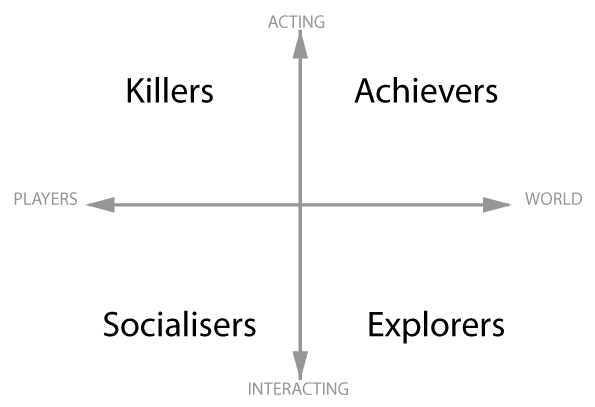
\includegraphics[scale=0.3]{figure/bartle.png}
    \caption{Bartle's taxonomy graph (adapted from \cite{bartle1996hearts}).}
    \label{fig:bartle}
\end{figure}
As it is clear in figure \ref{fig:bartle}, players that are of the Killer type will prefer games where actions involve other players, or NPCs (Non-Player Characters), while Achievers would prefer acting on the world and the environment. Socialisers and Explorer will favour interactions with other players or with the world, for example solving quests.
Even though it seems to be the most used model in game designing and game analysis, it does not seem to suit our purposes. This taxonomy fits the role playing scenario, but not the classical board games one. 
Agreeing with Bartle himself: it is not always the right tool for the job\cite{bartleyoutube}.
\subsection{Stewart's Unified Model}
In his article, Stewart analyzes a few different models -together with Bartle's- and matches all of them into a unified model\cite{stewart2011personality}. This shows how similar those models are, and that they could be almost interchangeable.
Since Bartle's model has been excluded from the list of the ones that are suitable for this project, the ones mentioned in Stewart's article have been excluded too. However, a brief description of Keirsey's model will be given further on in the chapter, as it will be useful for this thesis as a middle step for models adaptation.
\begin{figure}[H]
    \centering 
    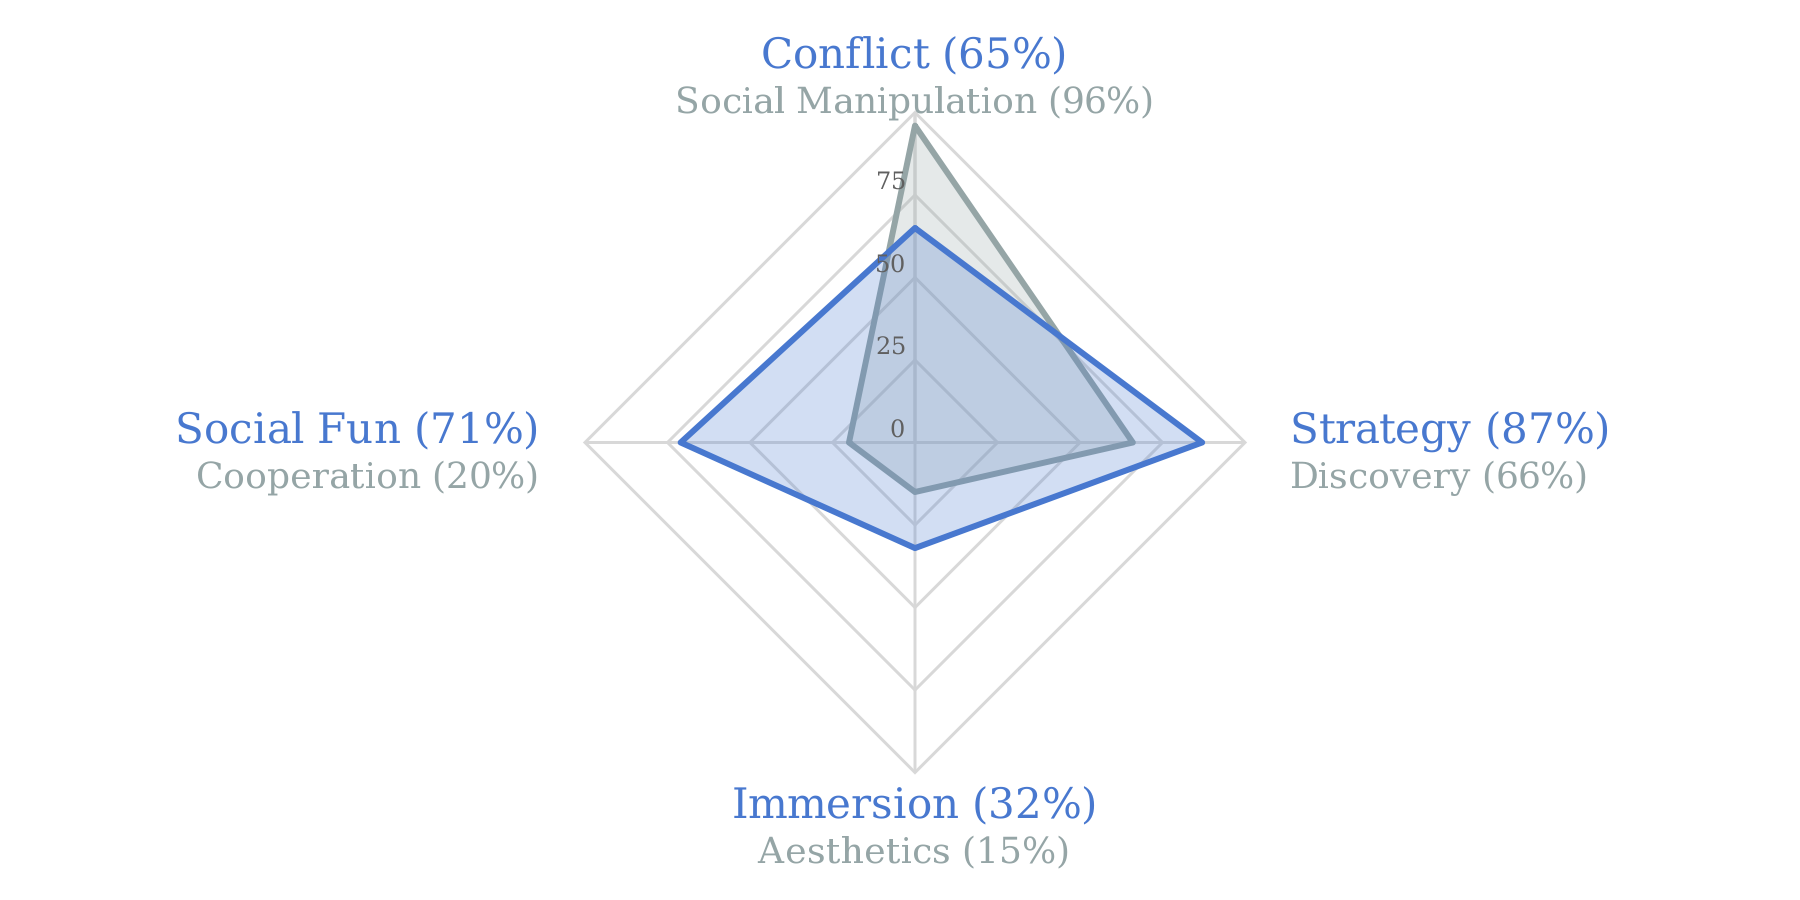
\includegraphics[scale=0.2]{figure/quanticfoundry.png}
    \caption{Example of Board Game Motivation Profile from Quantic Foundry\cite{chartprofile}.}
    \label{fig:quantic}
\end{figure}
\subsection{Quantic Foundry}
Quantic Foundry is a consulting company that works around psychology of gaming. They developed the Quantic Lab\cite{quanticfoundry}, which is a survey project aimed at understanding gamers preferences. They developed tools to test which gaming motivations are behind every player, and on their website there are two tests available, one for "Gamer Motivation Profile"\cite{yee2016gamer} and one for "Board Gamer Motivation Profile". As the first one is focused on videogames, it is outside of our scope.\\
In figure \ref{fig:quantic} can be seen an example of what are the results of the test. The profile gives a percentile rank across various motivations, as Conflict, Social Fun, Immersion and Strategy -and only secondly across Social Manipulation, Discovery, Aesthetics and Cooperation.
Even though the model seems to be pretty well-defined, it seems too complicated for this thesis' goal. It probably would be more appropriate if a bigger amount of data to work on would be available, so to force preferences over different types of games over the agent (i.e. the player that prefers immersive settings would not focus as well on classic board games, playing more sloppily that he would do if playing other games). Until the data is big enough, though, we prefer a simpler model.
\subsection{The Cardboard Republic Archetypes}
The Cardboard Republic is a website that collects board games news. They also have developed their own personality model, which consists of 6 different archetypes: Tactician, Socializer, Immersionist, Daredevil, Architect and Striker\cite{cardboard}. Their idea is to give an overview about those types, and suggest games that could be liked by the different personalities. There is a quiz on their website\cite{cardboardquiz}, and the model suggested here - based on gaming styles - seems to be highly appreciated among board gamers\cite{boardgamegeek}. 
\begin{figure}[ht]
    \centering
    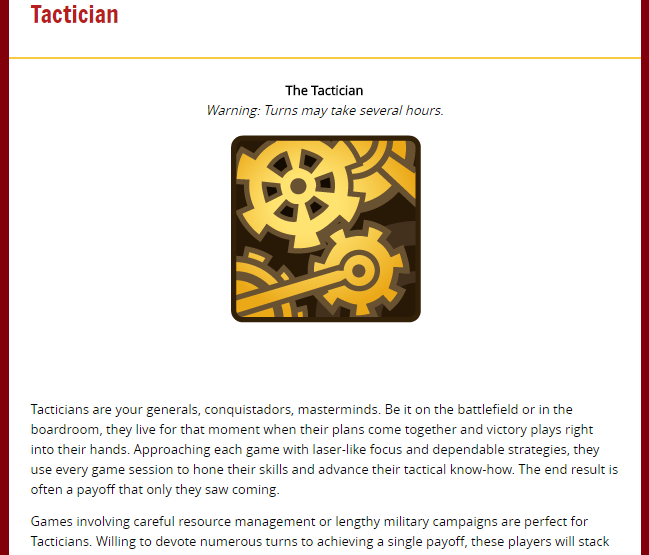
\includegraphics[scale=0.7]{figure/cardboard.png}
    \caption{Example of one of the Cardboard Republic Archetypes (from \cite{cardboard}).}
    \label{fig:cardb}
\end{figure}
In figure \ref{fig:cardb} is part of the description of the Tactician archetype, to give an idea about how the the different personalities are defined.
However, no academic resource about those archetypes has been found, limiting the credibility of being a valuable tool to use.
\subsection{Timmy, Johnny and Spike}
Timmy, Johnny and Spike are three different gamers personalities defined by Mark Rosewater and the "Magic: The Gathering" designers. It describes the three main different people that can be found while playing Magic.
Timmy defines the player who plays to enjoy "big" wins, Johnny is the player that prefers to win using hidden or peculiar strategies, and Spike is the competitive type that plays to win at all costs\cite{rosewater2002timmy}.\\
Even though this model would be simplistic enough to be used for this thesis, it feels like its is too tied to the "Magic: the Gathering" game, as it can be perceived even more in the "revisited" version of the same model\cite{rosewater2006timmy}, where the finer distinctions are based on the different behaviours of the players depending on the deck they are playing with.
It had been used as a personality model for other games, like Dominion\cite{gold2011trigram}, reaching the same conclusion about this model being game-dependent.
\subsection{BrainHex}
BrainHex is the tool developed by International Hobo Ltd to help categorize gamers while running a survey on their preferences.
They associate personalities with the parts of the brain responding to games in the specific classes, as can be seen in figure \ref{fig:brainhex}. 
\begin{figure}[ht]
    \centering
    
\includegraphics[scale=0.3]{figure/BrainHex_Classes.png}
    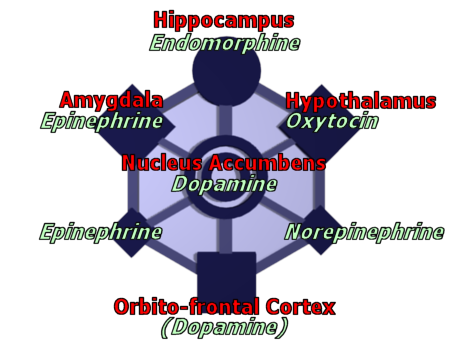
\includegraphics[scale=0.3]{figure/BrainHex_Brain.png}
    \captionsetup{justification=centering}
    \caption{On the left, BrainHex classes, on the right the corresponding parts of the brain (red text) and chemicals (green text) involved. Figure from \cite{nacke2011brainhex}.}
    \label{fig:brainhex}
\end{figure}
The personalities remind of the archetypes in the Cardboard Republic, and even though it has a more scientific background -results of a survey can be found in the article \cite{nacke2011brainhex}-, has the same complexity problem as some models described above.
\subsection{Big Five Personality Traits}\label{subsubsec:big5}
The Big Five Traits is a model widely used in psychology\cite{goldberg1993structure}, and it analyzes how personalities fall into five different scales: Openness, Conscientiousness, Extraversion, Agreeableness and Neuroticism. Each personality corresponds to a combination of the factors, helping the comprehension of behaviours and social interactions.\\
The five factors are describes as:
\begin{itemize}
\item \underline{Openness} (to experience): general openness towards emotions, new ideas, and non-ordinary situations. Low scores would imply favouring routines, and more traditional approaches.
\item \underline{Conscientiousness}: high self-discipline, sense of duty, aim for achievement. Lower scores describe careless behaviour, spontaneity, and impulsive reactions.
\item \underline{Extraversion}: higher scores imply talkativeness, sociability, and tendency to seek company of others. Lower scores describe reservedness and introversion. 
\item \underline{Agreeableness}: people with high scores are usually kind, trusting, trustworthy and considerate. Lower values imply skepticism, uncooperativeness and suspicion.
\item \underline{Neuroticism}: also called emotional instability, describe the tendency to experience negative emotions and be vulnerable to stress. 
\end{itemize}
Different scores in the factors match up in a range of various traits, giving a overall better fitting description of different personality.\cite{durupinar2008creating}\\
Unfortunately, it is not really suitable for this project, as all the factors matter equally and it would become too complicated to match users and gameplay behaviours to specific combinations. However, this was the model adopted by the project this thesis is being based on, therefore an adaption to this model was needed in order to have some continuity. A better understanding of this adaption will be given in subsection \ref{subsec:fourvsfive}. 
\subsection{Galen-Hippocrates' Four Temperaments}\label{sec:hippocrates}
Dating back to Hippocrates and Plato, the four temperaments might be one of the oldest personality models in psychology. It divides in four different categories: Sanguine, Melancholic, Phlegmatic, and Choleric\cite{merenda1987toward}. 
Shortly, the sanguine type is described as easily bored, somehow careless and as a risk-taker. Phlegmatic people are told to be diplomatic and to avoid conflicts. Cholerics are analytical, logical and goal-oriented. Melancholics are traditional and extremely ordered and accurate.
Even though there is a difference between temperaments and personality (the first one refers to innate behaviour, while the latter is built on top of the temperament, i.e. through experiences), we use the two terms interchangeably here, as what we are looking for is a simplistic model to categorize our players' behaviours.\\
Using the descriptions of each type as a guideline, and associating the model to the time responses for each type, as analyzed in \cite{chiappelli2005evidence}, those archetypes are manipulated a little, to get the results shown in table \ref{tab:temperaments} describing the playing style of each type. 
\begin{table}[ht]
    \centering
	\caption{Associated gaming skills to each of the four temperaments, in a scale from 1 to 4, where 1 means it is a strong suit for the type.}
    \scriptsize
    \begin{tabular}{|r|c|c|c|c|}
    	\hline
                        & Sanguine & Choleric & Melancholic & Phlegmatic  \\
        \hline
        Competitiveness & 3        & 1        & 2           & 4           \\
        Strategy        & 4        & 2        & 1           & 3           \\
        Analysis Paralysis      & 4        & 3        & 2           & 1           \\
        Contrasts       & 1        & 2        & 3           & 4           \\
        \hline
    \end{tabular}
    \label{tab:temperaments}
\end{table}
In table \ref{tab:temperaments} are shown the "specifics" for each personality type. A set of suits has been scaled from 1 to 4 depending on how fitting it is to each personality, where the suits are competitiveness, strategy, analysis paralysis and contrast, and they will be better described later. The scale system is applied instead of just pointing out if they are descriptive of the archetype or not in a binary fashion, in consideration of this not being exact, because of people showing different traits even if labeled with the same personality type. The table has the purpose not to strictly define a player type, but more to give an idea to our human players on what is to be expected from each temperament.
\begin{itemize}
    \item Competitiveness: shows how much a player cares about winning. It can be assumed that player types with a high value of competitiveness would do anything in order to win, without caring about how other players could perceive them. 
    \item Strategy: indicates if a player is careless in his moves or if there is a long-term plan behind. Players scoring high in strategy might play unintuitive or non-obvious moves, in order to satisfy the long-term plan. The lack of it might end up with more of short-term game (obvious moves, which give gain in the following few steps but not ultimately the best moves to win the game).
    \item Analysis Paralysis: high scores result in the player taking a long time between moves, possibly getting overwhelmed by the game and stalling.
    \item Contrast: if the player likes contrasts, it can be assumed it would play in a more aggressive and less defensive way, favouring risky moves over more conservative ones.
\end{itemize}
There are more distinctions that could be added to the table, but this already defines four very different playing styles and it feels it could be easily matched to our human players.
Unfortunately, the Phlegmatic type cannot really stand up for its skills in the games chosen in this project. A better perception of this type would be given with games that involve deception and contrast, like Werewolf\cite{werewolf} or the Resistance\cite{resistance}.
\subsection{Myer-Briggs}
The Myer-Briggs model distinguishes among 4 different bipolar traits: extroversion (E) and introversion (I), sensing (S) and intuition (N), thinking (T) and feeling (F), and judgment (J) and perception (P). It is assumed that people have a preference towards either ends of the scale, for each of those pairs, distinguishing then 16 different types of people\cite{myers2010gifts,myerbriggs}.\\ 
This model has being widely adopted in the business sector, although it is not considered as fully effective and reliable\cite{pittenger1993measuring,boyle1995myers}.
We have never considered this model as suitable for our purposes -having a too broad variety of classifications-, but since it is widely used in other contexts, we could find an adaptation between it and Keirsey's types\cite[p.~23]{keirsey1998please}.
\subsection{Keirsey's Temperaments}
Keirsey distinguishes between two basic human behaviours: communication and action. The first one could be further divided in either abstract or concrete, while actions could be defined as utilitarian or cooperative. The combination of those 4 traits forms the temperaments, which would be Artisans (concrete utilitarians), Guardians (concrete cooperators), Idealists (abstract cooperators), and Rationals (abstract utilitarians)\cite{keirsey1998please}.\\
Those four types can be further distinguished in 4 sub-types each, for a total of 16 different personalities that can be matched one-to-one to the Myer-Briggs' ones, as can be seen in table \ref{tab:keirsey-myers}.
\begin{table}[ht]
	\centering
    \scriptsize
	\caption{Keirsey's types and associated Myer-Brigg's types.}
    \begin{tabular}{|c|c|c|c|c|}
    	\hline
        Guardian & Artisan & Idealist & Rational\\
        \hline
        Supervisor & Promoter & Teacher & Fieldmarshal\\
        (ESTJ) & (ESTP) & (ENFJ) & (ENTJ)\\
        \hline
         Inspector & Crafter & Counselor & Mastermind\\
         (ISTJ) & (ISTP) & (INFJ) & (INTJ)\\
         \hline
         Provider & Performer & Champion & Inventor\\
         (ESFJ) & (ESFP) & (ENFP) & (ENTP)\\
         \hline
         Protector & Composer & Healer & Architect\\
         (ISFJ) & (ISFP) & (INFP) & (INTP)\\
		\hline
    \end{tabular}
    \label{tab:keirsey-myers}
\end{table}
This model was described in Steward's unified model\cite{stewart2011personality}, and being proposed as interchangeable with Bartle's taxonomy, not taken into consideration as base model for the project.\\
\section{General Game Playing}\label{sec:ggp}
Games have been found suitable for the development of Artificial Intelligence for many years now; in \cite{schaeffer2002games}, Schaeffer and van Der Herik present an interesting overview on the topic. In this project, we will focus on the branch called General Game Playing (GGP), firstly described by Pell's thesis\cite{pell1993strategy}. General Game Playing deals with agents learning new games without prior knowledge or ad-hoc strategy. The rules are given to the player only once the game has started, and the agent will have to work out a strategy while the match is ongoing. Contrarily to gaming agents like Deep Blue\cite{campbella2002deep} or AlphaGo\cite{silver2016alphago}, a General Game Player is not supposed to know a-priori any game-specific heuristic, and the heuristics it is supposed to be supplied with need to be applicable to any game, hence the word General. The subject includes a broad range of topics in AI, as knowledge representation, search algorithms, machine learning and, of course, game playing\cite{genesereth2014general}.
\subsection{Games Structure}
Innumerable games could be proposed to General Game Players, as long as they satisfy the common requirements: the games are supposed to have a fixed number of players, and can be defined as in definition \ref{def:game}.\\
\begin{definition}\label{def:game}
A game in GGP can be described as an automaton defined by a tuple ${<S,A,\delta,s_0,\Gamma, G_p>}$, where:
\begin{itemize}
\item ${S}$ is a finite number of states;
\item ${A}$ is a finite set of actions;
\item ${\delta}$ is the transition function, where ${\delta: S \times A \rightarrow S}$;
\item ${s_0}$ is the initial state, where ${s_0 \in S}$;
\item ${\Gamma}$ is the set of final states, where ${\Gamma \subseteq S}$;
\item ${G_p}$, the goal function associated to each player ${p}$, for each state $s \in S$.
\end{itemize}
\end{definition}
Only a subset of the games available for General Game Playing will be considered here: all of them are perfect information games, turn-dependent, and bounded to 2 players, as will be further described in section \ref{subsec:rulesgames}.
Games are represented with state machines (see appendix \ref{app:prel} for further information), specifically, they can be seen as trees, where each node-successor represents the legal moves from the parental node. Additionally, games are also Markov Decision Processes\cite{bellman1957markovian} -better described in \ref{sec:ml}-, as the history of transitions between states is irrelevant in the decision process for the future, at any given point\cite[p.~189]{genesereth2014general}.\\
When the game starts, the players are provided with the rules of the games, described in Game Description Language (GDL)\cite{love2008general} -a logic language, variant of Prolog. The language has recently been extended (GDL-II) to allow description of imperfect information games\cite{thielscher2010general,schiffel2011reasoning}.\\
In GGP, every game must be playable and weakly winnable - if multiplayer -, or strongly winnable - if single-player -, according to definitions \ref{def:playable} and \ref{def:winnable}, as found in \cite{genesereth2005general}.\\
\begin{definition}[Playability]
\label{def:playable}
A game is playable if and only if every player has at least one legal move in every non-terminal state.
\end{definition}
\begin{definition}[Winnability]
\label{def:winnable}
A game is weakly winnable if and only if, for each player, there is a sequence of joint moves of all players that lead to a terminal state where that player's goal is maximal. A game is strongly winnable if and only if, for some players, there is a sequence of individual moves that leads to a terminal state of the game where that player's goal value is maximal.
\end{definition}
The administration of the matches is left to the Game Manager, which communicates to and with the players regarding the ongoing game, i.e. informing when the respective turns start -passing over the state of the board and the list of previous actions-, or when the game is over. In figure \ref{fig:GGP} we can see the idea behind a GGP system\cite{genesereth2014general}.\\
\begin{figure}[H]
\centering
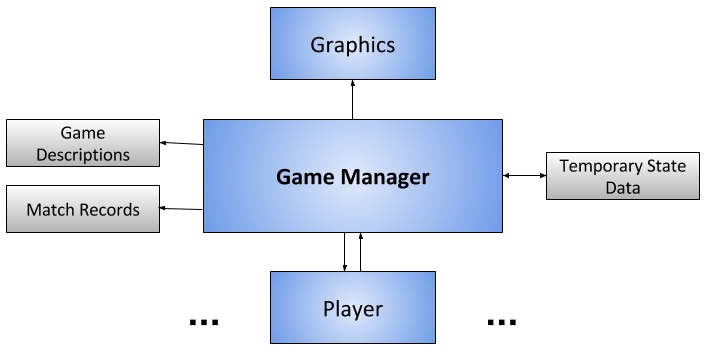
\includegraphics[scale=0.4]{figure/GGP2}
\caption{Diagram of a classical GGP environment (adapted from \cite{genesereth2014general}).}
\label{fig:GGP}
\end{figure}
The player used for this project uses a Monte Carlo Tree Search algorithm to find a strategy, and has been modified to go through already played games, and it will be further described in section 3.2.\\
\section{Monte Carlo Tree Search Algorithm}\label{sec:mctstheory}
Monte Carlo Tree Search has become more and more popular recently, due to the simplicity of implementation and the generality of application. It has been applied to a multitude of scenarios, giving satisfying results. Sticking to the games' development in the field of artificial intelligence, the Monte Carlo Tree Search algorithm has been applied to a variety of games: Go\cite{gelly2011monte,gelly2006modification,enzenberger2010fuego}, Hearts\cite{santoevaluating}, Settlers of Catan\cite{szita2009monte}, Amazons\cite{lorentz2008amazons}, and Lines of Action\cite{winands2010monte,winands2009evaluation} among the others. Moreover, it can also be associated with the best players participating in the General Video Game Playing Competition\cite{perez20162014}.
\\The algorithm has been developed starting from the idea of Monte Carlo methods, which obtain results relying on random sampling. In the search case, the Monte Carlo sampling is associated to a tree structure, where - when applied to games - each node represents a state in the game, and contains the current QValue and a value $n$, where $n$ is the number of visits for that specific state\cite{chaslot2008progressive}. The algorithm could be summarised in four main steps\cite{chaslot2010monte}, as can also be seen in \ref{fig:mcts}: 
\begin{enumerate}
\item \emph{Selection}: starting from root, and until a terminal node is hit, a leaf child node is recursively selected for expansion;
\item \emph{Expansion}: children nodes are added to the tree, depending on the available moves in the current state;
\item \emph{Simulation}: one play-out is run through until a value \emph{chargeDepth} limit is reached. A parameter \emph{epsilon} decides whether a random move is picked, or if MAST (Move-Average Sampling Technique, better described in the next paragraph) is applied.
\item \emph{Backpropagation}: the nodes in the tree get updated with the results from the simulation, associating a value $Q(s,a)$ to each node, defined as \begin{equation}\label{eq:mcts}
Q(s,a) = \frac{1}{N(s,a)} \sum_{i=1}^{N(s)} \chi_{i}(s,a) z_i
\end{equation}
where, using the same notation as \cite{gelly2011monte} and \cite{browne2012survey}, $N(s,a)$ is the number of times action $a$ has been simulated from state $s$, $N(s)$ describes how many times a game has been played out through state $s$, $z_i$ is the result of the $i$th simulation played out from $s$, and\\ $$\chi_{i}(s,a) = 
\begin{cases}
1 & \text{if }a\text{ was selected from state }s\text{ during $ith$ playout};\\
0 & \text{otherwise}.
\end{cases}$$
\end{enumerate}
\begin{figure}[ht]
    \centering 
    
\includegraphics[scale=0.4]{figure/MCTS.png}
    \caption{Iteration of MCTS (graph adapted from \cite{browne2012survey,chaslot2008progressive,winands2010monte}).}
    \label{fig:mcts}
\end{figure}
In the case of this project, the search ends when \emph{Limit} simulations - set as a constant $limit = 1000$ - is reached, but could be replaced by any time or memory constraints. 
\subsection{Monte Carlo Tree Search Enhancements}
The search can be associated to a set of other algorithms and tree policies, that can lead to quicker results compared to the basic Monte Carlo Tree Search, and might be preferred in some particular circumstances. In \cite{browne2012survey} we can find a comprehensive survey of the Monte Carlo Tree Search methods that have been implemented so far, and we would like to refer to it if the reader is interested in further information. Different enhancements can be applied at different stages of the search, it is then possible - and suggested - to apply multiple algorithm at once\cite{finnsson2010learning}; in our case, our algorithm uses UCT with RAVE and GRAVE as extensions for the learning process, and MAST as a search-control policy, and they will be better described later in this chapter. First thing, though, it is necessary to define what bandit problems are.
\subsubsection*{Bandit problems and Upper Confidence Bound (UCB)}
Bandit problems are a class of sequential decision problems that could be modeled over slot machines (known as "one-armed bandit" in Las Vegas), and describes the \emph{exploitation-exploration dilemma}, which is the problem of finding equilibrium between exploiting an action that appears to be optimal in the short run, and exploring the search space for a temporarily less-optimal but overall better one. Assuming to be in a room with $K$ slot machines, while having no knowledge of the past observations, our goal is to collect information about each slot machine by pulling their levers, while maximizing our cumulative reward at the same time. A K-armed bandit can then be described as a set of random variables $X_{i,n}$, with $1\leq i \leq K$ and $n\geq1$, and where $X_{i, n}$ represents the reward of pulling arm $i$ for the $n$th time. All $X_{i,n}$ are independent and identically distributed for all $n$, accordingly to an unknown distribution, with unknown mean $\mu_i$. Which bandit to play is decided with the aid of a \emph{policy}, whose goal is to minimize the regret of the player, defined as $\nu_n = \mu^*n-\mu_i \sum_{i=1}^{K}\mathbb{E}[T_i(n)]$, where $\mathbb{E}T_i(n)$ is the expected number of plays of arm $i$ in the first $n$ tries, and $\mu^*$ is the best possible reward\cite{browne2012survey,auer2002finite,kocsis2006bandit,kocsis2006improved,shivaswamy2012multi}. It is known that the slowest growing regret policy is $O(\ln n)$, as described by Lai and Robbins in \cite{lai1985asymptotically}, and one the simplest applicable policies, with expected logarithmic growth, is \emph{Upper Confidence Bound (UCB)}, first published by Auer et al. \cite{auer2002finite}, and defined as $$UCB1 = \overline{X}_i + \sqrt[]{\frac{2\ln n}{n_i}}.$$
\subsubsection*{Upper Confidence Bounds for Trees (UCT)}
Firstly proposed by Kocsis and Szepesvári \cite{kocsis2006bandit,kocsis2006improved}, UCT considers every state in the game as a multi-armed bandit problem, taking advantage of \emph{UCB1} and its simplicity and efficiency for the children selection. Then, the selection of child node $i$ depends on maximizing $$UCT = \frac{w_i}{n_i}+C_p*\sqrt[]{\frac{\ln N}{n_i}}$$ where $w_i$ is the number of wins after move $i$, $n_i$ is the number of simulations for move $i$, $N$ is the total number of simulations for the current node, and $C_p$ is a constant that we will be passing as a parameter called $ExplorationFactor$.
\subsubsection*{Rapid Action Value Estimation (RAVE)}
RAVE is part of policies that correspond to the name of \emph{All Moves As First} (AMAF)\cite{brugmann1993monte,helmbold2009all}. In this case, it is combined with UCT, as first done by Gelly and Silver\cite{gelly2007combining,gelly2011monte}, and it is meant to speed up the nodes' values evaluation, updating the value of each action every time it is taken, even in subsequent courses of action, and not only when it is specifically selected at one state. RAVE is based on a class of AMAF algorithms called $\alpha$-AMAF, which calculates the score for each action as $$\alpha Q_a+(1-\alpha)U$$ where $U$ is the UCT score, and $Q_a$ is the Q value for action $a$. In the RAVE case, we have a parameter $\beta$ instead of $\alpha$, which is calculated as $$\beta=\sqrt[]{\frac{Rave}{3*n+Rave}}$$ where $n$ is how many times the node has been selected, and $Rave$ is the value passed as parameter to our search, representing the number of visits a node can have before RAVE is not used anymore\cite{browne2012survey,gelly2007combining,gelly2011monte}.
\subsubsection*{General Rapid Action Value Estimation (GRAVE)}
GRAVE can be considered a generalization of RAVE, where a node is considered to have reliable statistics only when a certain number of playouts has been carried out. This value is passed as parameter $Grave$, and when the number of playouts is grater than it, then the values of the actions are calculated using general RAVE, otherwise the closest parent with a satisfying number of playouts is used as a reference to calculate the value for $Q_a$\cite{cazenave2015generalized}. 
\subsubsection*{Move Action Sampling Technique (MAST)}
The MAST method has firstly been described in \cite{finnsson2008simulation} and applied in CADIAPLAYER \cite{finnsson2007cadia}. This technique keeps track of the average value of each move, updated at backpropagation, and independent from the state it has been played in. From literature, it is known that, on the long run, actions $a$ with an higher average value $Q_{mast}(a)$ are most likely to be better than the ones with lower average\cite{finnsson2009simulation}. During playout the move selection can then be biased, with probability distribution corresponding to Gibbs distribution, as $$P(a) = \frac{e^{Q_{mast}(a)/\tau}}{\sum_{b=1}^n e^{Q_{mast}(b)/\tau}}$$ where $\tau$ is a parameter that controls the distribution, and $Q(a) = max GGP score = 100$, if $a$ hasn't been explored yet\cite{finnsson2008simulation,finnsson2007cadia,finnsson2009simulation}.
\subsubsection*{Discounting}
Two different discounts are applied to the moves values, controlled by two separate variables. One discount, depending on a variable called $ChargeDiscount$, applied at backpropagation, and the second discount, depending on $TreeDiscount$, is applied as a discount in the tree. It is thought that the search tree results are more reliable than the ones found at charge, therefore only a smaller discounting needs to be applied\cite{helgadottir2016virtual}.
\subsubsection*{Early Cut-Off}
Running Monte Carlo Tree Search algorithms might be time consuming, so a limit can be introduced to try to skim the moves that look more unappealing, so to focus better on the moves that are more promising\cite{finnsson2012generalized}. A limit $ChargeDepth$ is applied to the tree size, in order to make sure that a response to the opponent is being sent back in a decent amount of time. When this limit is hit by our search, a set of default values is returned, controlled by an array of variables called $ChargeDefaults$, one for each player\cite{helgadottir2016virtual}.
\subsubsection*{Heuristics}
Innumerable heuristics could be applied, either game-dependent (i.e. through piece counting\cite{helgadottir2016virtual}), based on the move selection history\cite{schaeffer1989history}, or used as personality bias. The latter is the case applied in this project's search, with two arrays of variables - one per each player - called $Aggressiveness$ and $Defensiveness$, and one value called $NiceThreshold$. As the names are mostly self-explicable, $Aggressiveness$ and $Defensiveness$ are controlling the goals of the game, being an increasing or decreasing factor, depending on the current state of the game. Considering that the maximum goal is $100$, and the minimum is $0$, we have that:
\begin{itemize}
\item If $goal_{current}>85$, the game can be considered as already won, and no biases are applied;
\item if $60<goal_{current}<85$, then the goal is biased using the $Aggressiveness$ value;
\item if $goal_{current}<35$, then the goal is biased using the $Defensiveness$ value;
\item if $35 \leq goal_{current} \leq 60$, then a value $r$ is picked uniformly at random in $[0,1]$ used to select with probability $P_{a,d}=0.5$ which bias to apply, $Aggressiveness$ or $Defensiveness$.
\end{itemize}
It is to be noted that $goal_{current}$ takes its value from the games rule, and most games only expect a win, a loss, or a draw, corresponding to 100, 0, or 50 points each. The values get then discounted, allowing to have some more flexibility with the $goal_{current}$ values described above.\\
Lastly, the value $NiceThreshold$ controls which difference in goals sets the AI to lower its standards and pick a sub-optimal move instead of the best one, to make the gaming experience more enjoyable for the opponent\cite{helgadottir2016virtual}.\\
Although those parameters have relatively less influence in the search outcome itself, it is easier to intuitively relate them to specific personality types. For example, looking back at table \ref{tab:temperaments}, a higher $Aggressiveness$ value would be expected for higher "Contrasts", hence for Sanguine users, as well as lower $NiceThreshold$ for more competitive players, as Choleric and Melancholic people are supposed to be.\\
\section{Machine Learning}\label{sec:ml}
Machine learning refers to the concept of extrapolating patterns and information from data. There are three main learning approaches that are applied in machine learning: supervised learning, where the agent learns to map certain outputs depending on specific inputs; unsupervised learning, where the agent is given an input and is meant to discover patterns in the outputs, so to be able to draw any conclusion about the data; and lastly, reinforcement learning, where behaviour is meant to be learnt depending on rewards or punishments. In the case of unknown reward functions that need to be withdrawn from observed behaviour, the problem becomes an inverse reinforcement learning one. In the case of this thesis, the problem falls in the supervised learning field. Classical methods for supervised learning could not be applied in this project, due to the complexity of the model used.
In this section will be defined the information needed to understand the Bayesian probability model in section \ref{sec:mlmethod}. A Bayesian approach simply means calculating each hypothesis' probability and using them to infer predictions from the data\cite{russell1995modern}.\\ The combination of a Bayesian framework and excerpting of preferences has gotten promising results in literature\cite{rothkopf2011preference}, as well the combination of Bayesian statistics and evolutionary algorithms, as for example in \cite{turner2012375}, where an Approximate Bayesian Computation algorithm (ABC) has been combined with a Differential Evolution one, in \cite{pelikan2003hierarchical}, where Bayesian Networks were used instead, or in \cite{wawrzynczak2014data}, where Bayesian Inference has been matched with Genetic Algorithms. 
\subsection{Decision Theory and Preference Elicitation}
Looking at the games' structure, it is easy to associate the problem of selecting the next move in a game to the topic of Decision Theory, which is an interdisciplinary field intuitively defined as the analysis of choices between options, each one having an expected utility value. The underlying idea in decision theory is called Maximum Expected Utility (MEU), where \emph{"an agent is rational if and only if it chooses the action that yields the highest expected utility, averaged over all the possible outcomes of the action"}\cite{russell1995modern}. In the specific, not having a full picture of the actions choices for all states of each game, the problem tried to be solved in this thesis falls in the class of "Decision Making Under Uncertainty", which, as the name hints, refers to the problems where either information or knowledge are incomplete\cite[p.~3-4]{scholz1983decision}. Even more specifically, the goal to extract preferences depending on the personality of the player would fit in the Preference Elicitation problem, as it tries to identify the favourite events of a group of people, over the set of available actions that can be selected from being in a certain state, depending on the group's personality. The choices throughout games are here extracted from a Monte Carlo Tree Search algorithm, described previously, which has a set of controlling parameters the actions picked depend on. Different sets of parameters lead to different actions, hence the decisions should be able to be associated to a set of MCTS parameters. This set is meant to be found using a Genetic Algorithm -described later in this chapter-, with a fitness function that represents the expected utility function mentioned earlier.
Our hypothesis is assuming multiple major differentiation of people's behaviour in game playing, based on specific personalities. We are expecting that games played by people with different personality would develop with different types of underlying strategies, than if compared to people with the same personality. The implementation of our algorithm is foreseeing the application of a diverse set of parameters, depending on the personality of the player.\\
\subsection{Markov Decision Process}
It has been mentioned in \ref{sec:ggp} that the games in General Game Playing are seen as Markov Decision Processes. In order to clarify what a Markov Decision Process is, it is necessary to start defining the Markov property. Let $I$ be a state-space, $X$ is a random variable with values in $I$ where $X:\Omega\rightarrow I$, then $$\lambda_i=\mathbb{P}(X=i)=\mathbb{P}({\omega : X(\omega)=i}).$$
It is said that $(X_n)_{n\geq 0}$ is a Markov chain with initial distribution $\lambda$ and transition matrix $H=(h_{ij}:i,j \in I)$ if
 \renewcommand{\labelenumi}{(\roman{enumi})}
\begin{enumerate}
\item $X_0$ has distribution $\lambda$;
\item for $n\geq 0$, conditional on $X_n=i$, $X_{n+1}$ has distribution $(h_{ij}:j\in I)$ and is independent of $X_0,\cdots X_{n-1}$.
\end{enumerate}
\begin{theorem}
A discrete-time random process $X_{n_{0\leq n \leq M}}$ is a Markov chain ($\lambda$,H) (or just called Markov($\lambda$,H)) if and only if $\forall i\ i_1,\cdots,i_N\in I$ $$\mathbb{P}(X_0=i_1, X_1=i_2,\cdots,X_N=i_N)=\lambda_{i_1}h{i_1i_2}h{i_2i_2}\cdots h{i_{N-1}i_N}.$$ 
\end{theorem}
Additionally:
\begin{theorem}
Let $(X_n)_{n\geq 0}$ be Markov$(\lambda,H)$. Then, conditional on $X_m=i$, \\$(X_{m+n})_{n\geq 0}$ is Markov$(\delta_i,H)$ and is independent of the random variables $X_0,\cdots,X_m$.
\end{theorem}
The proofs are let to be read in \cite{norris1998markov}, where we have taken the cue from for the above theorems and definitions. However, more informally speaking, the Markov property is assuming that the Markov Chain $X$ is in a current state $s_t$, then no additional information is given by how $s_t$ has been reached. Therefore, the current state $s_t$ provides enough information for the reward to be computed without looking at previous states. Subsequently, Markov Decision Process can then be defined as sequential decision processes with a Markovian transition function and a reward function\cite{russell1995modern}. More formally, adapting from \cite{puterman2014markov} and \cite{ng2000algorithms}:
\begin{definition}
A (finite) Markov Decision Process (MDP) is a tuple \\$<S, A, P_{sa}, G_.(\cdot,\cdot),\xi>$, where:
\begin{itemize}
\item $S$ is a finite set of states;
\item $A$ is a finite set of actions;
\item $P_{sa}(\cdot)$ are the state transition probabilities upon taking action $a$ in state $s$;
\item $G_p(s,s')$ is the reward function;
\item $\xi\in[0,1]$ is the discount factor.
\end{itemize}
\end{definition}
\section{Genetic Algorithm}\label{sec:gatheory}
The information to be inferred from the dataset is a set of parameters which can be used as input to an agent, expecting that the output actions will match humans', when the human has the same personality as the agent being trained. In order to do determine this specific set of parameters, an optimization algorithm is applied over the fitness function \ref{eq:mcts}. The approach adopted is a Genetic Algorithm.\\ Genetic Algorithms (GA) are part of the family of stochastic optimization methods, and are based on Evolutionary Algorithms, having the purpose to study the adaptation of individuals throughout time. First implemented by John Holland and his colleagues and students between 1960s and 1970s\cite{holland1992adaptation}, there has been a growing interest in the topic in the past years. Evolutionary Algorithms take their terminology from biology, being inspired by it in the first place. The concept of \emph{population} is then introduced as a set of \emph{individuals}. Each \emph{individual} has a \emph{chromosome}, formed by a set of \emph{genes}. A more detailed description of the biological terminology can be found in \cite[p.~5]{mitchell1998introduction} and in \cite[p.~35]{wahde2008biologically}, while here the vocabulary will be limited to what is strictly related to the purposes of this project.\\Genetic Algorithms are finite, however, the outputted solution might be due to premature convergence, and only be a local optima, therefore there is no complete certainty of finding the actual optimal solution. 
\subsection{General Structure}
There is no final definition of GAs, but a general structure can be drawn from literature:
\begin{itemize}
\item \emph{Individual}: a set of \emph{genes}. The \emph{genes} have a defined \emph{encoding scheme}, that can be binary encoding scheme, strings, real numbers, integers, and so on. 
\item \emph{Population}: a family of $\Psi$ individuals is initialized at random, forming the first \emph{generation} of the population.
\item \emph{Fitness function}: is a function $F$ whose value is calculated at evaluation time. The overall goal of optimization problems is to maximise (or minimise) the value of this function.
\item \emph{Evaluation}: each \emph{individual} $i$ is evaluated, after being decoded in the relative variable, and the value of $F(i)$ is calculated, where $F$ is the \emph{fitness function}, and $i=1,...,\Psi$.
\item \emph{Selection}: in order to form the next \emph{generation} it is needed to select which \emph{individuals} will survive evolution, and which will not. There are multiple strategies for selection, where the more popular are tournament selection, roulette-wheel selection and ranking selection. Those methods will be further described in subsection \ref{subsec:selection}.
\item \emph{Elitism}: keeping track of our best individual generation after generation reduces the risk of having a decreasing fitness due to mutation or crossover. It has been shown that combining elitism to a selection algorithm improves the final results\cite{baluja1995removing}.
\item \emph{Crossover}: the reproduction of the individuals happens through a crossover algorithm, where, once two parents are picked, two new individuals containing genes from either parents are added to the next generation. Further information about the topic can be found in subsection \ref{subsec:cross}.
\item \emph{Mutation}: Once the new generation is born, a mutation can happen to none, one or multiple genes in each individual. A description of how mutation happens over this project's encoding can be found in \ref{subsec:mut}.
\end{itemize}
\subsection{Selection}\label{subsec:selection}
In this section, three different algorithms for the selection process will be described. Only the roulette-wheel selection has been used in this thesis, as specified in \ref{sec:ga}, but the other two algorithms have been considered and might have been applied for comparison if there were no time constraints.\\
\textbf{Tournament selection}\qquad
Tournament selection, as the name hints, it is the selection process carried out as a tournament. Once defined a tournament size $t_s$, $t_s$ individuals are taken and compete for survival. The lower $t_s$ is, the higher the competition. This flexibility makes this approach one of the most widely used in GAs\cite{miller1995genetic}.\\
\textbf{Roulette-wheel selection}\qquad
The roulette-wheel strategy selects individuals proportionally to their fitness value. To obtain the resemblance with an actual roulette-wheel, a cumulative fitness function is calculated as $$\phi_j=\frac{\sum^i_{j=1} F(j)}{\sum^\Psi_{i=1} F(i)},\hfill j=1,...,\Psi$$ where $F(i)$ is the fitness value of individual $i$. A value $r$ is drawn uniformly at random in $[0,1]$, and the individual with the smallest $j$ that satisfies $r<\phi_j$ is selected\cite{wahde2008biologically}. \\
\textbf{Rank selection}\qquad
Firstly defined in \cite{baker1985adaptive}, it ranks all the individuals depending on the value of their fitness function, from rank $\Psi$ for the best individual, to $1$ for the worst. Each individual $i$ has then an associated probability of being selected, calculated as $$P(i)=\frac{1}{\Psi}\big(\eta^-+(\eta^+-\eta^-)\frac{i-1}{\Psi-1}\big);\hfill i\in{1,...,\Psi}$$ where the conditions $\eta^+=2-\eta^-$ and $\eta^-\geq0$ are satisfied, since the population size is constant, and $\frac{\eta^-}{\Psi}$ is the probability of selecting the worst individual in this generation's population, while $\frac{\eta^+}{\Psi}$ is the probability of selecting the fittest\cite{blickle1995comparison}.
\subsection{Crossover}\label{subsec:cross}
Here, the most used crossover algorithms will be described; the first, because we think it helps to have a better understanding of the crossover process, and a second one, which is the algorithm that has applied in this project. Further techniques can be found in \cite{umbarkar2015crossover}.\\
\textbf{Single Point Crossover}\qquad
A popular way of applying crossover is to decide on a "barrier" $c$, and create the offspring $o_1$ and $o_2$ with $c$ genes from one of the parents, and $(G-c)$ genes from the other one, where $G$ is the total number of genes in an individual. This approach is called Single Point, and it is represented in figure \ref{fig:crosssp}.
\begin{figure}[H]
    \centering 
    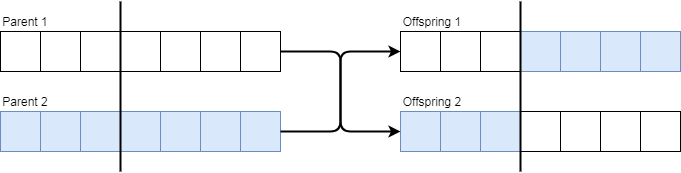
\includegraphics[scale=0.5]{figure/Crossoversinglepoint.png}
    \caption{Example of Single Point crossover between two individuals.}
    \label{fig:crosssp}
\end{figure}
Deriving from this idea, there is Two-Points crossover, as well as Multi-Points Crossover, which explanation at this point is trivial.\\
\textbf{Averaging Crossover}\qquad
Given two individuals as parents, this approach returns two children $o_1$ and $o_2$ with genes calculated as an average from the parents' $p_1$ and $p_2$, as $$g_{o_1} = \alpha g_{p_1} + (1-\alpha)g_{p_2}$$ and $$g_{o_2} = (1-\alpha) g_{p_1} + \alpha g_{p_2}$$ where $\alpha$ is chosen uniformly at random in $[0,1]$\cite{ladkany2012genetic}, for each gene $g$.
\subsection{Mutation}\label{subsec:mut}
Any gene in any individual could be subjected to mutation, depending on probability $P_{mut}$. When dealing with genes encoded with real numbers, the most common approach for mutation is the real-number creep, where a creep value limits the range of values the new gene can take. Let $C_r$ be the creep rate, then the new gene is $$g\Leftarrow g-\frac{C_r}{2}+C_r\gamma=g+C_r(\gamma-\frac{1}{2})$$ where $\gamma$ is picked uniform at random in $[0,1]$\cite[pp.~53-55]{wahde2008biologically}.
\subsection{Termination} 
GA usually stops when there is stagnancy: either the fitness function has not been increasing for generations, or the individuals converged to very similar ones (leading to a very similar fitness function too). In other cases it is preferred to give a fixed number of generations to run the GA for; in other, a decency fitness test is added, stopping the algorithm when a minimum fitness value is reached, finding an acceptable result instead of the optimal one. In this project, a stagnancy test has been adopted, and it will be further described in section \ref{sec:ga}.


% METHODS
\chapter{Methods}
This chapter will contain the methodologies applied during the development of this project. Firstly, in section \ref{sec:defprob} there will be the definition of the problem this thesis tries to solve. The selected personality model to be applied in the project is described in section \ref{sec:persmodme}, followed by the explanation of how the data has been collected, in section \ref{sec:datacolme}. Section \ref{sec:baseprojme} introduces the base project, that is the baseline for the artificial agent the algorithms implemented in this thesis are training upon. The description of the gaming algorithm involved will be found in section \ref{sec:mctsmet}, which is a Monte Carlo Tree Search algorithm. Section \ref{sec:mlmethod} includes the probability model in association with our problem. The Genetic Algorithm used to infer information from the dataset can then be found in section \ref{sec:ga}. Lastly, the evaluation of the set of parameters outputted by the above mentioned algorithms can be found in section \ref{sec:meteval}.
\section{Problem Definition}\label{sec:defprob}
The aim of this thesis project is to understand if procedural personæ can be inferred from human game playing, and if it is possible to recreate those personalities by parameters tuning of a Monte Carlo Tree Search algorithm, so to return the optimal move for each state, where optimal in this case means similar to the human player's moves. A set of parameters $\vec{\theta_j}$ would return action $a_j^s$ for a state $s$, while -for the same state $s$- we can expect a different $a_k^s$ for parameters $\vec{\theta_k}$. What we aim to show by the end of this project, is that for a personality $\rho$, we can have a set of parameters $\vec{\theta}_\rho$ that leads the artificial agent to pick the same actions (or equivalent), as a human with personality $\rho$. In order to find the values associated to those set of parameters, we will apply a Genetic Algorithm over the Monte Carlo Tree Search, expecting the optimal set of parameters to match a set of training data.
Finally, each set of parameters $\vec{\theta_\rho}$ will be evaluated on new clusters of data, part of which is of unknown users (with relatively unknown personalities), and part of known testers. The influence that the choice of parameters $\vec{\theta}$ will have on the search outcome, matching or not the correct personality, will confirm or disprove our thesis.
\section{Personality Model}\label{sec:persmodme}
After an extensive research over personality models, the Galen-Hippocrates' model became the best suited for this project, as it seems like different players could be easily mapped to a specific type, giving us some variety and not too subtle distinctions. Furthermore, there is academic background, that gives it some reliability as a model.
Some other models, like BrainHex, or the Big Five, give a more accurate representation of personalities, however the expected amount of data to be retrieved will not give them justice.
Every model listed above could succeed in different settings, but they are either too complicated for our scopes, or they are not backed up by enough academic research to be used as reliable models.
\section{Data Collection}\label{sec:datacolme}
When dealing with Optimization Algorithms and Machine Learning, it is usually suggested to have a discrete amount of data available. Knowing how slow data collection could be, the best option for us would have been to find existing gameplay databases. Unfortunately, as the existing platforms were unresponsive, or the data was just not suitable for our purposes, this research was unsuccessful. Consequently, we set up our own data collection system, taking advantage of the Tiltyard server\cite{tiltyard} as framework. \\
The Tiltyard server has been developed as a testbed for general game players, which also implies it not meant to be strictly used by human players. Because of the not extraordinarily user-friendly interface, we had to provide our testers with an instruction file\cite{datacollection}, as well as a couple of social platforms (a Facebook group and an IRC Channel, to be specific) to find opponents to play against. 
Additionally, in order to keep track of the personalities of the players, we asked our testers to fill a questionnaire with the information not collected by the Tiltyard server, such as usernames, perceived personality of the adversary, and player's own personality.\\
In the instruction file\cite{datacollection}, the testers can find a brief description of the personality models, with a table representation (see table \ref{tab:temperaments}) to help them define their own archetype, the rules of the games, as explained in subsection \ref{subsec:rulesgames}, together with the actual instructions on how to use Tiltyard.\\
To simplify the game set-up process, we have implemented a second version of the Tiltyard homepage, including the choice of playing against the latest version of CadiaPlayer\cite{cadiaplayer, finnsson2007cadia, bjornsson2009cadiaplayer}, a player previously developed at Reykjavik University. However, time constraints have not played in our favour, and the page has not been available to the public early enough to make any actual difference in the data collection process. \\
The participation in the data collection has not been very high, even after organizing periodic events trying to simplify finding an opponent. Only a small amount of games were played in total, but we managed to gather an acceptably uniform distribution of games and personalities, as will be better described in section \ref{subsec:dataresults}.
\subsection{Selected Games}\label{subsec:rulesgames}
The games selected are two players, perfect information games: Checkers, Nine Board Tic-Tac-Toe, Connect Four, and Skirmish. In figures \ref{fig:checkers}, \ref{fig:9boardttt}, \ref{fig:connect4}, and \ref{fig:skirmish} we can see examples of the games while ongoing. Although a few of those games cannot be considered new for our testers, the version implemented in Tiltyard might have included a few variants of the rules as they are traditionally known.\\
The choice of games has been dictated by the list of available games in Tiltyard; once we selected the ones with a usable human interface, we checked the average number of moves.
\subsubsection*{Checkers}
The game is played on a 8x8 squares chessboard, where each player has 12 pieces. The goal of the game is to capture all the adversary pieces by jumping over them. Pieces can move only diagonally, and on unoccupied squares. In this version of the game, capturing is not mandatory, and it is possible to capture multiple pieces during the same turn (if there is an empty square between every two). When a piece reaches the adversary's side of the board, it becomes a “king”, and gains the ability to move backwards. The player who has no more pieces on the board, or cannot move anymore, loses the game (see figure \ref{fig:checkers}).
\begin{figure}[H]
\centering
	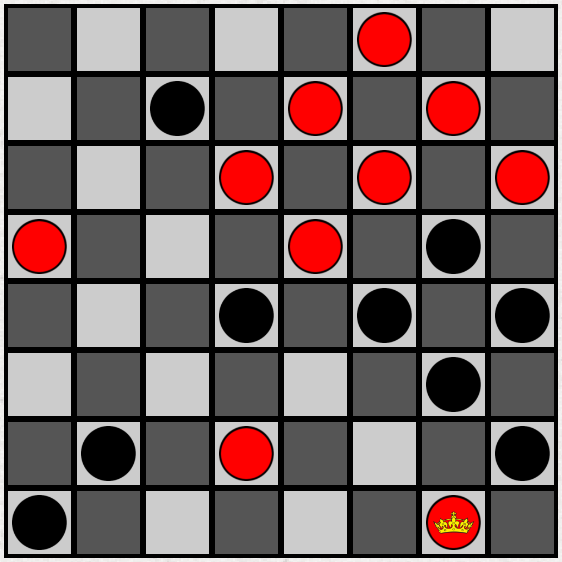
\includegraphics[scale=0.35]{figure/checkers}
    \caption{A game of Checkers.}
    \label{fig:checkers}
\end{figure}
Checkers has been selected because it is a classic game, where non-simple strategies can be developed. It is also the most time consuming game among our choice, having 99.91 moves on average for each game on Tiltyard\cite{checkers}.
\subsubsection*{Nine Boards Tic-Tac-Toe}
The game is played on a grid formed by 3x3 simple Tic-Tac-Toe grids. The first player can play on any board, but his/her choice would force the second player to play in the grid corresponding to the square of the previous move (if player 1 picks the central square, player 2 will have to play in the central grid). If the grid the current player is supposed to play on is full, then any other move is allowed. To win, the player has to win on any one of the boards (see figure \ref{fig:9boardttt}).
\begin{figure}[H]
\centering
	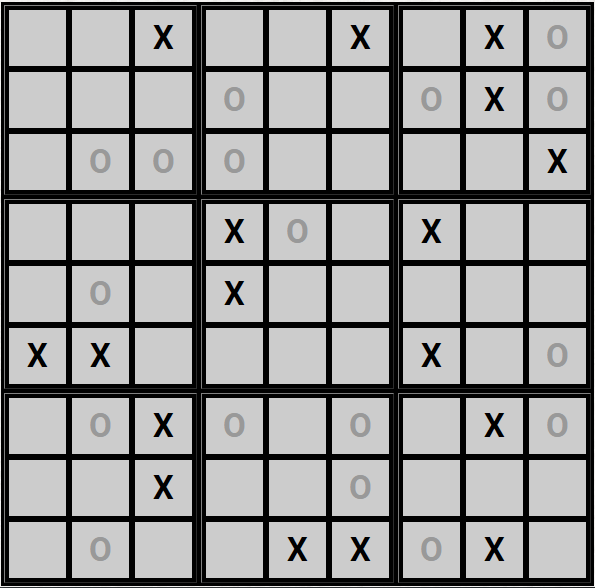
\includegraphics[scale=0.35]{figure/9boardstictactoe}
    \caption{A game of Nine Boards Tic-Tac-Toe.}
    \label{fig:9boardttt}
\end{figure}
Nine-Board Tic-Tac-Toe has 35.07 moves on average on Tiltyard\cite{nineboards}, and has been chosen because it is a variant of the more famous Tic-Tac-Toe, with the advantage of not having the risk of having too obvious moves.
\subsubsection*{Connect Four}
The game is played on a 6x8 suspended grid. Taking turns, the players drop a token of their colour in the grid. The goal is to have 4 tokens connected either horizontally, vertically, or diagonally (see figure \ref{fig:connect4}).
\begin{figure}[H]
\centering
	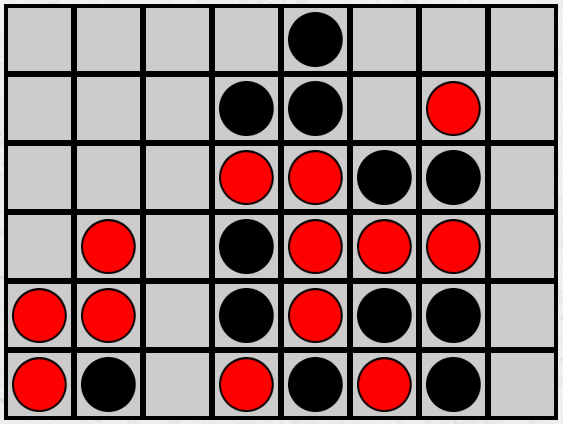
\includegraphics[scale=0.35]{figure/connectfour}
    \caption{A game of Connect Four.}
    \label{fig:connect4}
\end{figure}
Connect Four has been selected for being the "quick game", with only 28.52 moves on average on Tiltyard\cite{connect4}, and being mostly well known worldwide.
\subsubsection*{Skirmish}
The game uses a chessboard and the same pieces as chess, which are also moving in the same way. The pieces are all worth the same, fixed, amount of points -from the pawn to the king-. To win, the player has to eat the most amount of adversary’s pieces. The game terminates when all the pieces of one player have been eaten, or one of the players cannot move anymore. The rules of chess are not rules in Skirmish (i.e. it is not possible to castle, there is no check mate, and so on...), however pawns get promoted to queens when they reach the other side of the chessboard (see figure \ref{fig:skirmish}).
\begin{figure}[H]
\centering
	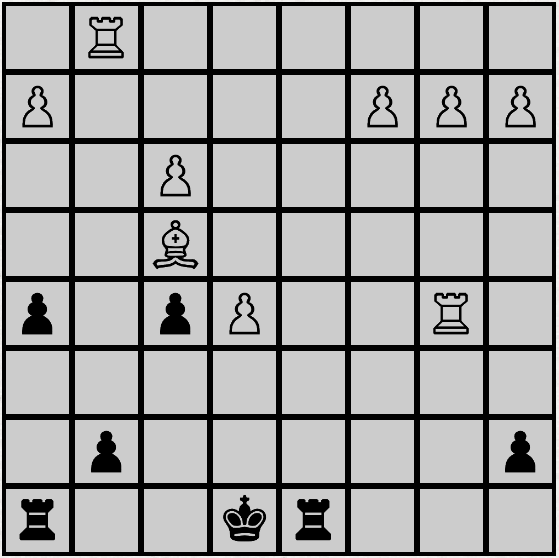
\includegraphics[scale=0.35]{figure/skirmish}
    \caption{A game of Skirmish.}
    \label{fig:skirmish}
\end{figure}
Skirmish has been chosen later in the thesis project, taking the place of another game that had been selected first (called Battle), but was proving to be problematic for our users to play. We then decided that a chess-like game, without falling into the obvious choice of chess, was the perfect game for our evaluation process, having a wide tree search as a consequence of its complexity. Only a handful of matches have been played on Tiltyard, so we do not think that the average number of moves of 59.67\cite{skirmish} is a reliable statistic. 
\section{Base Project}\label{sec:baseprojme}
The implementation of this thesis project has been based on a work with the title of "Virtual General Game Playing Agent"\cite{helgadottir2016virtual}, previously carried out at Reykjavik University. The authors have joined the General Game Playing features with a Unity Player who would mimic human behaviours when playing a game of Checkers or Nine Men's Morris. The player has a virtual reality interface, as we can see in figure \ref{fig:virtualagent}, and it is meant to work with a joystick device and an Oculus Rift. Although the graphic interface is fascinating, we have not taken advantage of it, focusing only on the back-end GGP Engine.\\
\begin{figure}[ht]
\centering
	
\includegraphics[scale=0.3]{figure/virtualagent}
    \caption{A screen-shot of the Virtual Agent while playing a game of Checkers.}
    \label{fig:virtualagent}
\end{figure}
The back-end implementation is based on the ggp-base framework\cite{schreiber2013general}, which provides API for the Game Manager, supplying libraries to handle the GDL reasoner and the communication protocol, to create the game state machines, and to check which moves are legal at each state. This framework has been improved with the addition of a Monte Carlo Tree Search algorithm, tweaked depending on a wide set of parameters that are supposed to give the virtual player a human-like gaming style. Those parameters are the ones that are exploited in the current version of the search, and are described in detail in section \ref{subsec:param}.\\
The Monte Carlo Tree Search is paired with an heuristic dependent on the number of pieces on the board, which would affect the aggressiveness or defensiveness of the virtual player's next moves. However, having a more diverse selection of games in our implementation, we are not adopting the same heuristic, relying on the evolutionary algorithm to find a suitable balance in the 17 control parameters.\\
Lastly, in order to make the virtual agent more human, it has been provided with the choice of a personality. When starting the game, the user can select values to decide which personality the opponent will have. The personality model used here is the Big Five, described in subsection \ref{subsubsec:big5}, and in subsection \ref{subsec:fourvsfive} we can associate the "older" model with the one chosen for the purposes of this thesis' work.
\section{Monte Carlo Tree Search}\label{sec:mctsmet}
The search to evaluate which move needs to be played is implemented as a Monte Carlo Tree Search algorithm with UCT. The algorithm satisfies the requirement of not being game-dependent, and has been giving optimal results in the gaming AI development. In section \ref{sec:mctstheory} we have seen the theory behind it and described the different strategies that can be applied to a basic Monte Carlo Tree Search Algorithm, while in this section we will understand the settings chosen for our purposes.\\
We run our Monte Carlo Tree Search over each game sample, with a set of 17 different parameters that will affect the values in the tree and, possibly, the output. Those parameters could be hand picked and hard coded (as they were in the old project we based this thesis on), or chosen by the evolutionary algorithm described in section \ref{sec:ga}. As mentioned earlier, our algorithm is implemented allowing the addition of RAVE and GRAVE over UCT, MAST, and other enhancements, as early cut-offs, some personality-biased heuristics, and discounting.\\
Our algorithm runs over the matches collected, calculating the QValues for all the moves in each state, but eventually forcefully selecting the same move as the user. This is done to give us an easier way of mapping human behaviour over the states available, focusing only on the knowledge we have available.
\subsection{Parameters}\label{subsec:param}
The Monte Carlo Tree Search parameters are what truly affects the values of each move, as we said earlier. Since each parameter represents and controls a different piece of structure in the search, it is easy to assume that each of them will have its own variable type and a range of meaningful values. More details about the intervals are given in section \ref{sec:ga}. \\
The parameters can be described as:
\begin{itemize}
	\item $Rave$ is the threshold at which only the QValues are considered for selecting moves, and Rave stops being used.
	\item $Grave$ is the threshold setting when Grave stops being used, and only general Rave is used for moves evaluation.
	\item $Charge Depth$ represents the depth limit for a play out.
	\item $Horizon$ represents the maximum depth of the tree.
	\item $Exploration Factor$ is a UCT value that controls the exploration weight over exploitation in the MCTS algorithm.
    \item $Limit$ is the number of simulations the MCTS executes. It has been fixed to be $Limit = 1000$, and will not be modified at any stage during the process.
	\item $Tree Discount$ decides how much discount there is on every move after expanding a node in the tree.
	\item $Charge Discount$ represents the discount applied after each play out.
	\item $Epsilon$ represents the probability of using MAST instead of picking a random move.
    \item $Charge Defaults$ is a couple of default values to be applied if a charge is stopped in early stages.
	\item $Defensiveness$ is a pair of values (one per each player) that bias the goal over valuing defensive moves.
	\item $Aggressiveness$ is a pair of values (one per each player) that bias the goal towards aggressive moves.
    \item $Random Error$ represents the probability of picking a random move instead of the best one.
    \item $Nice Threshold$ biases the move selection, forcing the AI to not always pick the best move and becoming a too strong opponent.
\end{itemize}
The parameters $Defensiveness$, $Aggressiveness$, and $Charge Defaults$ are represented in the search as arrays of 2 items each, one per player. That explains the discrepancy between the number of parameters mentioned earlier, and the number of items in the description list here above.
\section{Probability Model}\label{sec:mlmethod}
In this section the probabilistic model will be described, applying a Bayesian approach. Recapitulating, a set of parameters is plugged into a MCTS algorithm, whose outcome changes the game actions. A dataset of several games where players can be distinguished depending on a personality is given as input. Let a set of uniformly distributed parameters - within different ranges, as described in section \ref{sec:ga} - be defined as $\vec{\theta} = {\theta_1,\ldots,\theta_L}$, where $L$ (where we know $L=17$); $\vec{\rho} = {\rho_1,\ldots,\rho_4}$ indicates any among the people's personalities; and $D_{mcts}^k$ with $k=1,\ldots,M$, is the match data retrieved from the MCTS, where $M$ is the number of matches played. The set of matches associated to a specific personality $\rho$ will be indicated as $M_\rho$. It should also be distinguished from $D_h$, which refers to the human gameplay data that has been collected, with $h=1,\ldots,M$. As a simplification, we will refer to $\rho$ as any of the four personalities, as it is not necessary to singularly specify them in this context, and to $\vec{\rho}$ as the set of all personalities in the model. We refer to Appendix \ref{app:prel} for a brief summary of the probability rules applied in this section.\\
Overall, it is in the interest of this project to confirm the thesis where \begin{equation}\label{eq:thesis}
P(\vec{\theta}) \neq P(\vec{\theta}|\rho), \qquad \forall \rho \in \vec{\rho}
\end{equation} as otherwise we would be proving that the set of parameters $\vec{\theta}$ used will not be relevant to distinguish a common pattern in the behaviour of a user with personality $\rho$. Additionally, it would be favorable that $D_h=D_{mcts}^k,\  \forall h,k \in [1,\cdots,M]$ in other words, it would be optimal to have a set of moves resulting from the MCTS that would match human actions.\\
In figure \ref{fig:BN} is the Bayesian Network representation of the problem, so to help clarify the following statements.
\begin{figure}[H]
\centering
\begin{tikzpicture}[->,>=stealth',shorten >=1pt,auto,node distance=2.8cm, semithick]

  \node[state]	(A)              {$\rho$};
  \node[state]	(B) [right of=A] {$D$};
  \node[state]	(C) [right of=B] {$\vec{\theta}$};

  \path (A) edge	node {} (B)
        (B) edge	node {} (C);
\end{tikzpicture}
\caption{Bayesian Network representation.}\label{fig:BN}
\end{figure}
The goal is to find the probability of $P(\vec{\theta}|\rho)$ over all the set of data, where $$P(\vec{\theta}|\rho) = \int_{1}^{M_\rho} P(\vec{\theta}|D_h^j)P(D_h^j|\rho).$$ Due to the sample-size of our dataset, however, that is equivalent to saying $$P(\vec{\theta}|\rho) = \sum_{j=1}^{M_\rho} P(\vec{\theta}|D_h^j)P(D_h^j|\rho).$$ Starting from the last term of the chain, let $$P(D_h|\rho) = \frac{P(\rho | D_h)P(D_h)}{P(\rho)}.$$ It is assumed that $P(\rho|D_h)=1$ if the personality $\rho$ matches the data $D_h$, or  $P(\rho|D_h)=0$ otherwise. When the dataset matches the personality, it is then obtained that $$P(D_h|\rho) = \frac{P(D_h)}{P(\rho)}.$$ Considering uniform probability over the personalities $\rho$, it is given that $P(\rho)=\frac{1}{4}$, concluding that 
\begin{equation}\label{eq:1}
P(\vec{\theta}|\rho) = \frac{1}{4}\sum_{j=1}^{M_\rho} P(\vec{\theta}|D_h^j)P(D_h^j)
\end{equation} where the matches considered are the one corresponding to the personality $\rho$ considered. The set of games $[1,M_\rho]$ for a specific $\rho$ will from now be referred as $D_\rho$. Rewriting equation (\ref{eq:1}) it is then obtained that \begin{equation}\label{eq:2}
P(\vec{\theta}|\rho) = \frac{1}{4}P(\vec{\theta}|D_\rho)P(D_\rho).
\end{equation}
From equation (\ref{eq:2}) the \emph{posterior} is defined as $P(\vec{\theta}|D_\rho)$, as the probability of having a specific set of parameters $\vec{\theta}$ matching a set of matches $D_\rho={D_h^1,D_h^2,\cdots,D_h^{M_\rho}}$. 
Considering all matches in each set, the probability that needs to be maximised, can be defined as $$P(\vec{\theta}|D_\rho) = \frac{P(D_\rho|\vec{\theta})P(\vec{\theta})}{\sum_{\vec{\theta_j}} P(D_\rho|\vec{\theta_j})P(\vec{\theta_j})}.$$
The problem of maximising the posterior can be reduced to maximising the numerator, as the denominator is the sum over all the possible data and parameters' sets and is constant. Furthermore, $P(\vec{\theta})$ is the \emph{prior} of our model, constant as well, and defined as $$P(\vec{\theta})=\frac{1}{W}$$ where $W$ is the cardinality of the set of all possible parameters $\vec{\theta}$.
Hence, the maximisation problem has scaled down to \begin{equation}\label{eq:argmax}
	\argmax_{\vec{\theta}} P(D_\rho|\vec{\theta})
\end{equation} which happens to be the \emph{likelihood} of the model, where $D_\rho$ indicates all the matches belonging to the same set, defined over a specific personality $\rho$. In other words, it is the probability of selecting a list of certain actions given a set of parameters.\\ Being the games defined as Markov Decision Processes, the likelihood for each match $D_h$ can then be calculated as \begin{equation}\label{eq:likelihood}
P(D_h|{\vec{\theta}}) = P_{\vec{\theta}}(a_1,...,a_T| s_1,...,s_T) = \prod_{t=1}^{T} P_{\vec{\theta}}(a_t|s_t)
\end{equation}
where $T$ is the number of turns in the match, and $P_{\vec{\theta}}(a_t|s_t)$ is the probability of choosing action $a$ in state $s$, in turn $t$. It is to be noted that, on a higher level, multiple actions could be available for selection in any state $s$, due to the non-deterministic policy of the games. \\
The probability of a human player selecting an action $a_{human}$ in a certain state $s$ is calculated using the Boltzmann-Gibbs distribution - which is often associated to multi-armed bandit problems\cite{coulom2006efficient}, hence applicable to MCTS - as $$P_{\vec{\theta}}(a_{human}|s_t) = \frac{e^{Q_{\vec{\theta}}(a_{human},s_t)\kappa}}{\sum_{j=1}^{A}e^{Q_{\vec{\theta}}(a_j,s_j)\kappa}}$$ where $\kappa=0.1$ is a constant, $Q_{\vec{\theta}}(a_{human}, s_t)$ is the Q-value the search with parameters $\vec{\theta}$ has associated to action $a_{human}$ in turn $t$, $A$ is the total of all legal actions at current state, and $Q_{\vec{\theta}}$ is the Q-value of said actions, as calculated from equation (\ref{eq:mcts}).\\
The optimal outcome of the chosen set of parameters for a specific personality would be to have $$P_{\vec{\theta}}(a_{mcts}|s_t) = P_{\vec{\theta}}(a_{human}|s_t)$$ where  in the same state $s_t$, for any state $t \in [1,\ldots, T]$, it is true that $a_{human}=a_{mcts}$.\\
To maximise equation \ref{eq:argmax}, we assume that $P(D_\rho|\vec{\theta})$ can be approximated by the product of $P(D_h|\vec{\theta})$ over all the matches $D_h$ in $D_\rho$, for ease of calculation. That is defined as the fitness function $F(\vec{\theta})$ for the genetic algorithm,  where $\vec{\theta}$ will - in the GA case - be an individual $i$. The fitness is then defined as: \begin{equation}\label{eq:fitnessfunc}
F(\vec{\theta}) = \sqrt[M]{\prod_{m=1}^{M}\sqrt[T]{\prod_{t=1}^{T}P_{\vec{\theta}}(a_{human}^{t,m}|s_{t,m}))}}
\end{equation} where $T$ is the number of turns in each match, $M$ is the number of matches gone through, and, for each state $s$, $a_{human}^{t,m}$ is the action chosen by the human player. It is easy to notice that the fitness function is the geometric mean over all the matches of the probability of selecting the action $a_{human}$ picked by the human player in state $s$. The fitness function uses the geometric mean over the matches in order to normalise the fitness over matches with different number of turns, and the different cardinality of the sets $M_\rho$, for each $\rho\in\vec{\rho}$.
\\The set of parameters $\vec{\theta}$ that derives the likelihood for each set of data $D_i$ is, however, unknown. The optimization method used to find the values applicable to the $\vec{\theta}$ is a Genetic Algorithm with a population of individuals $\vec{\theta}$ and the likelihood (\ref{eq:likelihood}) is utilised as fitness function that needs to be maximised.\\
\section{Genetic Algorithm}\label{sec:ga}
We have tried to solve the optimization problem with the implementation of a Genetic Algorithm, as we previously mentioned in section \ref{sec:gatheory}. \\
We have taken a population of $\Psi=100$ individuals, where each individual has a set of chromosomes $c_i$, where $i=1..17$, representing the parameters of the Monte Carlo Tree Search, described in subsection \ref{subsec:param}, and initialized uniformly at random, in a given interval. Each chromosome's value is allowed to be in a meaningful range, and will be  better described at the end of this section.\\
Each individual is used as parameters to run the search and, once the moves are selected, the fitness $F(i)$ is evaluated as the geometric mean of the Boltzmann-Gibbs distribution function over every turn - or state $s$ - of each match, using equation (\ref{eq:fitnessfunc}) proposed earlier, and repeated here for completeness:
\begin{equation*}
F(\vec{\theta}) = \sqrt[M]{\prod_{m=1}^{M}\sqrt[T]{\prod_{t=1}^{T}P_{\vec{\theta}}(a_{human}^{t,m}|s_{t,m}))}}
\end{equation*} where $T$ is the number of turns in each match, $M$ is the number of matches gone through, and, for each state $s$, $a_{human}^{t,m}$ is the action chosen by the human player. For the GA purposes, $\vec{\theta}$ will be referred to as individual $i$.
Different fitness functions could have been applied in order to possibly find a better fitting one, however, only equation (\ref{eq:fitnessfunc}) has been considered due to time limitations.\\
The selection uses a roulette wheel approach, where each individual has probability $$P(i) =\frac{F(i)}{\sum_{j=1}^{\Psi}F(j)}$$ of being selected, where $F(i)$ is the fitness value of individual $i$. The cumulative probability distribution is then calculated over all the individuals as $$C=\sum^\Psi_{j=1}F(j)$$ and a value $r$ is picked uniformly at random in $[0,1]$. If $$\frac{\sum^{i-1}_{j=1} F(j)}{C}< r < \frac{\sum^{i}_{j=1}F(j)}{C}$$ then $r$ sets the minimum threshold for selecting a specific individual, and individual $i$ is picked. The roulette-wheel method has been preferred over the other selection algorithms, because of its non-biased approach\cite{chipperfield1997introduction}.\\
Taking two selected individuals at the time, we apply crossover with probability $p_c = 0.05$. In case the crossover will not be carried out, the individuals remain unchanged. We will be using averaging crossover, because of its closest analogy with actual genetics\cite{ladkany2012genetic}. Recapitulating, the gene $g$ of the offsprings $o_i$ is derived from the genes of parents $p_i$, and is defined as: $$g_{o_1} = \alpha g_{p1} + (1-\alpha)g_{p2}$$ and $$g_{o_2} = (1-\alpha) g_{p_1} + \alpha g_{p_2}$$ where $\alpha$ is chosen uniformly at random in $[0,1]$ for each gene.\\
Mutation has probability $p_{mut} = 0.1$ to happen, with a creep rate $C_r = 0.4$, which represents the width of the distribution. We are adopting a uniform distribution to apply the creep mutation, so the new gene would be obtained as $$g_m = g - \frac{C_r}{2} + C_r \gamma$$ where $\gamma$ is uniformly distributed between $[0,1]$.\\
The values of $p_{c}$, $p_{mut}$ and $C_r$ have been tuned with few testing over a set of the available games, and have been selected depending on the resulting number of generations, in order to try to avoid premature convergence.\\
The algorithm continues evolving the population, until it becomes stagnant, or one of the individuals reaches an acceptable fitness $f_a = 0.9$. To define a population as stagnant, we first calculate the variance of the chromosomes in all the individuals of the current population, as $$\sigma^2_i = \frac{\sum_{j=1}^{\Psi}\left({\frac{g_j^i-g^i_{\mu}}{\sup(g^i)-\inf(g^i)}}\right)^2}{(\Psi-1)}$$ where $g_j^i$ is the $i$th gene in individual $j$, $g^i_{\mu}$ is the average value for gene $i$, with $i = [1...C]$ and $j = [1...\Psi]$, where $C$ is the number of chromosomes and $\Psi$ is the population size. The population is considered then stagnant when $$max_{i, j}^{C, \Psi}(\sigma_i) <= \sigma_a$$ where $\sigma_a = 0.005$ is what we can consider an acceptable standard deviation for our gene's values pool.\\
When the algorithm stops, the fittest individual will be the best set of parameters to represent the personality of that gameplay set, being it the one with the highest likelihood.
\subsection{Parameters Intervals} This paragraph contains details about the values each gene in the chromosome can possibly take. It is to be reminded that each gene represents a MCTS parameter, as have been described in section \ref{sec:mctsmet}.
The genes are then said to be:
\begin{itemize}
\item long $Rave$, where $Rave \in [0,(y*Limit)]$, with $y$ a small integer constant, and $limit$ the number of simulations the search runs for (for us, $y=5$ and $Limit=1000$);
	\item long $Grave$, where $Grave \in [0, 120]$;
	\item long $Charge Depth$, where $Charge Depth \in [0,100]$;
	\item long $Horizon$, where $Horizon \in [1,20]$;
	\item long $Exploration Factor$, where $Exploration Factor \in [1,UCT_{limit}]$, with \\$UCT_{limit} = \overline{\Lambda_J}+\sqrt[]{\frac{2 \ln n}{n_i}}$, where $\overline{\Lambda_j}$ is the average reward for the state $j$, $n$ is the number of simulation so far, and $n_i$ is the number of simulations after the $i$th move. We can approximate $UCT_{limit}=140$;
	\item double $Tree Discount$, where $Tree Discount \in [0.9,1]$;
	\item double $Charge Discount$, where $Charge Discount \in [0.9,1]$;
	\item double $Epsilon$, where $Epsilon \in [0,1]$;
    \item double[2] $Charge Defaults$, where $Charge Defaults[i] \in [35.00,45.00]$;
	\item double[2] $Defensiveness$, where $Defensiveness[i] \in [0,3]$;
	\item double[2] $Aggressiveness$, where $Aggressiveness[i] \in [0,3]$;
    \item double $Random Error$, where $Random Error \in [0,1]$;
    \item float $Nice Threshold$, where $Nice Threshold \in [0,100]$.
\end{itemize}
The types of the variables refer to Java primitive data types\cite{javadatatypes}, where \emph{long} is a 64-bit two's complement integer, \emph{double} is a double-precision 64-bit IEEE 754 floating point, \emph{float} is a single-precision 32-bit IEEE 754 floating point, and with the notation \emph{[2]} we indicate arrays of 2 elements, or the element of index $i$ if indicated as \emph{[i]}.
\section{Evaluation}\label{sec:meteval}
The evaluation process involves the Skirmish games not used for training, of which we have user-associated personalities, and a set of games from the 2013 and 2014 match archives available on the GGP researchers' website\cite{researchggp}. The archives have been filtered, leaving us with human-played games, with no errors in the match, and that are either completed, or with an acceptable number of moves - to avoid considering games that have been aborted only after a couple of turns. \\ 
Once recovered the winning individuals from the Genetic Algorithm, the evaluation matches are run through both with the correct parameters, and with random ones, calculating the Action Agreement Ratio (AAR)\cite{holmgaard2015monte}, which is the percentage of matching moves between the users' results and the search's. We also calculate $\Delta_Q = Q(a_{human}) - Q(a_{search})$, where $Q(a)$ is the Q-value associated to action $a$ in state $s$. The magnitude of $\Delta$ will be significant to evaluate if the parameters we plugged in are having any influence.\\
The results of the evaluation process will be further discussed in the results chapter \ref{sec:reeval}.

% RESULTS
\chapter{Results}\label{sec:results}
This chapter collects the results along the stages of this thesis project. In section \ref{subsec:fourvsfive} is a comparison between the personality model of choice and the base project's, so the interested user can translate the personality-based results to either works. In section \ref{subsec:dataresults} are collected the results from the data collection. The output from the Genetic Algorithm will be discussed in section \ref{sec:gares}. Lastly, the results from the evaluation process will be discussed in section \ref{sec:reeval}.
\section{Comparison of Personality Models}\label{subsec:fourvsfive}
It has been mentioned in section \ref{subsubsec:big5} that the original project this thesis is basing itself on adopted the Big Five as personality model. Due to its complexity, it is harder to be applied in this context, therefore a comparison of the two models, the Big Five and the Four Temperaments, had to be searched upon. Unfortunately, such direct comparison does not seem to be directly available. We then compare Galen-Hippocrates' four types to Keirsey's and then to Myers-Briggs.\\
It is easy to find association between Keirsey's types, Galen-Hippocrates' and Myer-Briggs', as for example in Keirsey's book\cite{keirsey1998please}.  In table \ref{tab:keirsey} we can see a summary of those types, and how they are equated to each other.
\begin{table}[H]
	\caption{Comparison of Galen-Hippocrates' Four Temperaments with Keirsey's Four Temperaments and Myer-Briggs personality types, as from \cite{keirsey1998please}.}
    \centering
    \scriptsize
    \begin{tabular}{|c|c|c|c|c|}
    \hline
    Models & \multicolumn{4}{|c|}{Types} \\
		\hline
        \hline
        Galen-Hippocrates & Sanguine & Choleric & Melancholic & Phlegmatic\\
        \hline
        Keirsey & Artisan & Idealist & Guardian & Rational\\
        \hline
        Myer-Briggs & E\textbf{S}T\textbf{P} & E\textbf{NF}J & E\textbf{NT}J & E\textbf{S}T\textbf{J} \\
       				& I\textbf{S}T\textbf{P} & I\textbf{NF}J & I\textbf{NT}J & I\textbf{S}T\textbf{J} \\
                    & E\textbf{S}F\textbf{P} & E\textbf{NF}P & E\textbf{NT}P & E\textbf{S}F\textbf{J} \\
                    & I\textbf{S}F\textbf{P} & I\textbf{NF}P & I\textbf{NT}P & I\textbf{S}F\textbf{J} \\
        \hline
        Common traits Myers-Bryggs & SP & NF & NT & SJ \\
        \hline
    \end{tabular}
    \label{tab:keirsey}
\end{table}
There has been a study to correlate the Myers-Briggs types to the Big 5, and the results are described in \cite{mccrae1989reinterpreting}, and shown in table \ref{tab:big5mb}. The results were collected by a population of 267 men and 201 women, and it was found that the correlation values for men and women have negligible difference. Hence, we can just as well consider the results gathered from the men population, and consider it valid.
Given table \ref{tab:keirsey}, we can easily define a table with the probability of being any of the Myer-Briggs types, given the Galen-Hippocrates', and it can be seen in table \ref{tab:prob-myers-galen}.
\begin{table}[H]
    \caption{Correlation of Big 5 factors with Myer-Briggs (data from \cite{mccrae1989reinterpreting}).}
    \centering
    \scriptsize
    \begin{tabular}{|c|c|c|c|c|}
    \hline
    \multirow{2}{4em}{Big 5} & \multicolumn{4}{|c|}{Myer-Briggs} \\
    \cline{2-5}
         & E-I & S-N & T-F & J-P\\
        \hline
        \hline
        Neuroticism & 0.16 & -0.06 & 0.06 & 0.11\\
        \hline
        Extraversion & -0.74 & 0.10 & 0.19 & 0.15 \\
        \hline
       	Openness & 0.03 & 0.72 & 0.02 & 0.30 \\
        \hline
		Agreeableness & -0.03 & 0.04 & 0.44 & -0.06 \\
        \hline
		Conscientiousness & 0.08 & -0.15 & -0.15 & -0.49 \\
        \hline
    \end{tabular}
    \label{tab:big5mb}
\end{table}
\begin{table}[H]
	\caption{Probability of each Myer-Briggs preferences given the Galen-Hippocrates' type.}
   	\centering
    \scriptsize
    \begin{tabular}{|c||c|c||c|c||c|c||c|c|}
    	\hline
    	& E & I & N & S & F & T & J & P\\
      	\hline
        Choleric & 0,5 & 0,5 & 1 & 0 & 1 & 0 & 0,5 & 0,5\\
		\hline
        Sanguine & 0,5 & 0,5 & 0 & 1 & 0,5 & 0,5 & 0 & 1\\
        \hline
		Phlegmatic & 0,5 & 0,5 & 0 & 1 & 0,5 & 0,5 & 1 & 0\\
		\hline
        Melancholic & 0,5 & 0,5 & 1 & 0 & 0 & 1 & 0,5 & 0,5\\
        \hline
    \end{tabular}
    \label{tab:prob-myers-galen}
\end{table}
\begin{table}[H]
    \caption{Extension of table \ref{tab:big5mb}, with clarification of the preferences scale.}
	\centering
    \scriptsize
    \begin{tabular}{|c||c|c||c|c||c|c||c|c|}
    	\hline
    	& E & I & N & S & F & T & J & P\\
        \hline
		Openness & 0 & 0,03 & 0,72 & 0 & 0,02 & 0 & 0 & 0,3\\
        \hline
		Conscientiousness & 0 & 0,08 & 0 & 0,15 & 0 & 0,15 & 0,49 & 0\\
        \hline
		Extraversion & 0,74 & 0 & 0,1 & 0 & 0,19 & 0 & 0 & 0,15\\
		\hline
		Agreeableness & 0,03 & 0 & 0,04 & 0 & 0,44 & 0 & 0,06 & 0\\
        \hline
		Neuroticism & 0 & 0,16 & 0 & 0,06 & 0,06 & 0 & 0 & 0,11\\
		\hline
    \end{tabular}
    \label{tab:correlationExtended}
\end{table}
Table \ref{tab:correlationExtended} shows the same values as in table \ref{tab:big5mb}, just written in a way that emphasises the correlation values of each of the Myer-Briggs preferences, given the Big 5 types.\\
Finally, the relation between tables \ref{tab:prob-myers-galen} and \ref{tab:correlationExtended} can be calculated.
Let $J$ be a matrix containing the values in table \ref{tab:prob-myers-galen}, and $K$ be a matrix containing the values in table \ref{tab:correlationExtended}. Then it can be said that $$R=JK^T$$ where $R$ shows the correlation between the Four Temperaments and the Big 5, and which values can be seen in table \ref{tab:results}.
\begin{table}[H]
    \caption{Correlation between the Four Temperaments and Big 5.}
    \scriptsize
	\centering
	\begin{tabular}{|c|c|c|c|c|c|}
    	\hline
		& Openness& Conscientiousness & Extraversion & Agreeableness & Neuroticism\\
        \hline
		Choleric & 0,905 & 0,285 & 0,735 & 0,525 & 0,195\\
        \hline
		Sanguine & 0,325 & 0,265 & 0,615 & 0,235 & 0,28\\
        \hline
		Phlegmatic & 0,025 & 0,755 & 0,465 & 0,295 & 0,17\\
        \hline
		Melancholic & 0,885 & 0,435 & 0,545 & 0,085 & 0,135\\
		\hline		
	\end{tabular}
    \label{tab:results}
\end{table}
\begin{figure}[H]
\centering
	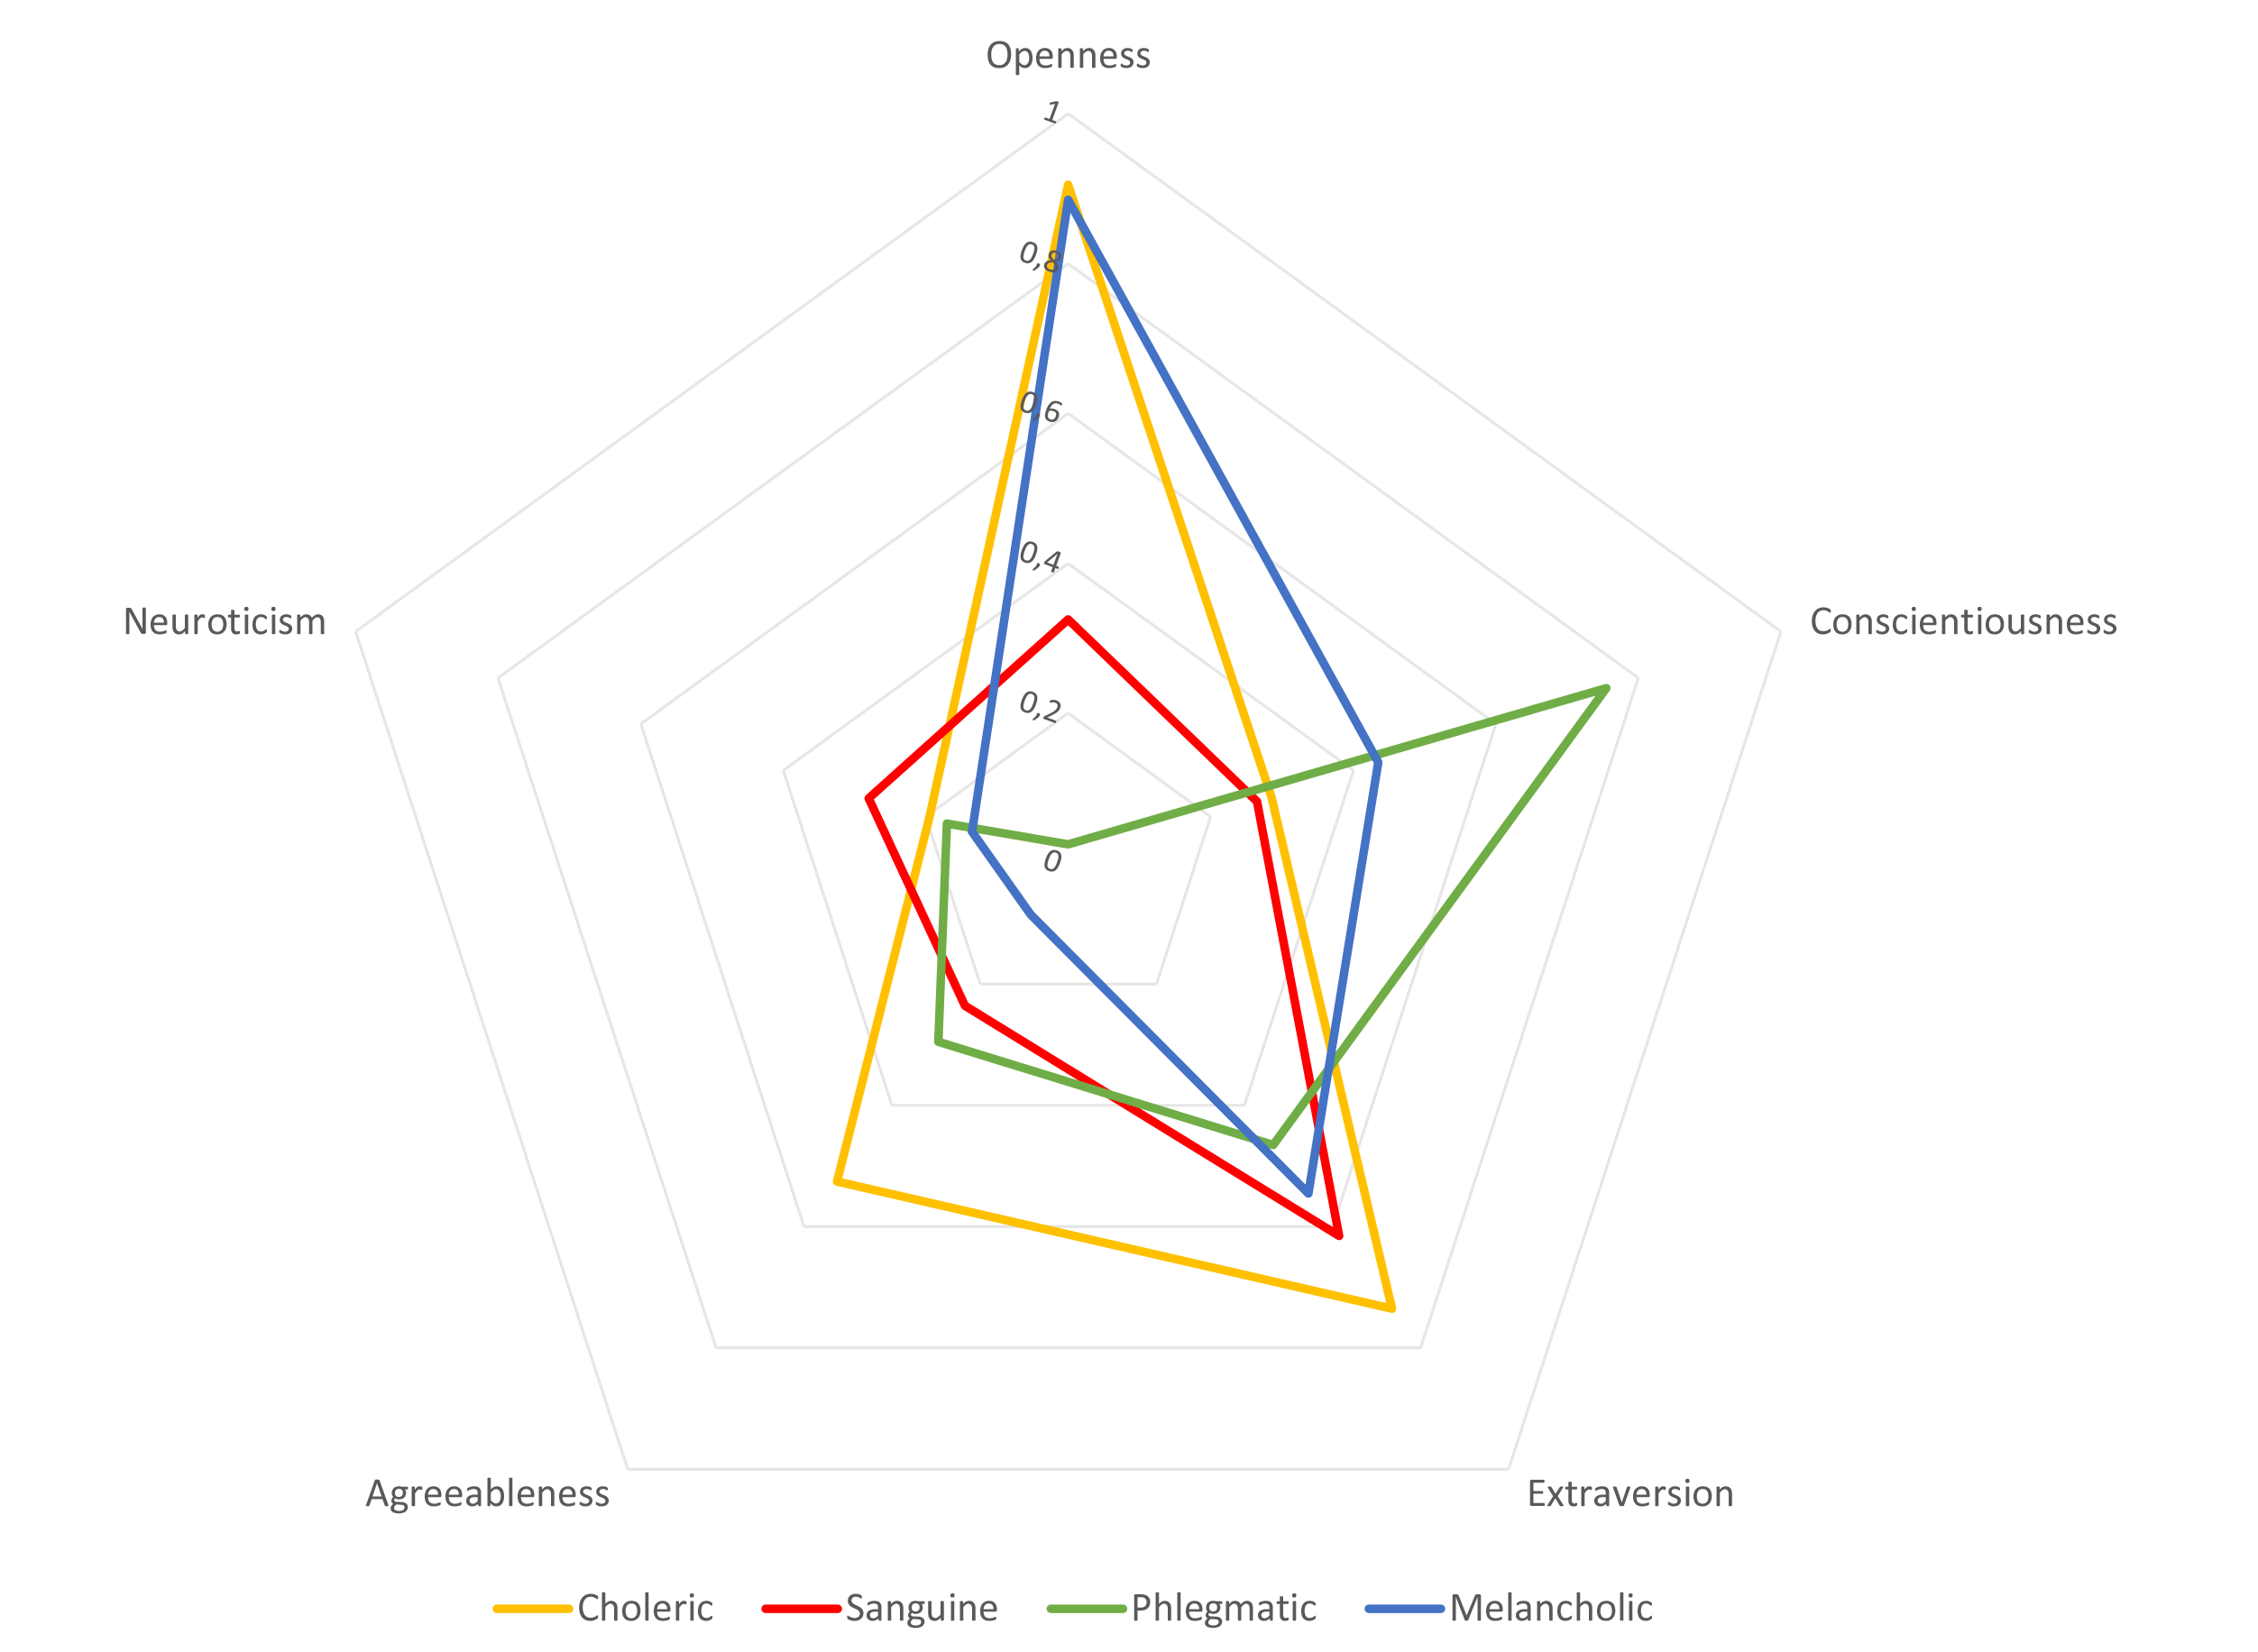
\includegraphics[scale=0.15]{figure/graph1}
    \caption{Correlation between the Four Temperaments and Big 5 factors.}
    \label{fig:all4}
\end{figure}
In figure \ref{fig:all4} we can see the comparison between all the temperaments, while in figure \ref{fig:4t-big5} we can see the temperaments singularly.
Since the old project allows only three settings for each of the Big 5 traits (low, medium, high), we thought it could be useful to normalize the results in \ref{tab:results} in a scale 0-2, and consequently round up at the closest integer. The results are shown in table \ref{tab:normalized}.
\begin{table}[H]
	\caption{Correlation of Big 5 factors with Myer-Briggs (table \ref{tab:results}) normalized to 2.}
	\centering
    \scriptsize
    \begin{tabular}{|c|c|c|c|c|c|}
    	\hline
    	& Openness & Conscientiousness & Extraversion & Agreeableness & Neuroticism\\
        \hline
        Choleric & 2 & 1 & 1 & 1 & 0\\
        \hline
		Sanguine & 1 & 1 & 1 & 0 & 1\\
		\hline
		Phlegmatic & 0 & 2 & 1 & 1 & 0\\
		\hline
		Melancholic & 2 & 1 & 1 & 0 & 0\\
		\hline
    \end{tabular}
    \label{tab:normalized}
\end{table}
The conclusion that can be drawn from looking at the results, is that the Neuroticism value is mostly irrelevant for the Four Temperaments model, nonetheless, we believe it might influence the game play, proving in this way that the chosen personality model is not complete to represent human behaviour properly in the general game play field. However, the magnitude of data collected for this project reduced the option of utilising any other complicated model, which would maybe be more suitable for modeling human behaviour in games.
\begin{figure}[ht!]
\centering
    \subfloat[Choleric graph][Choleric] {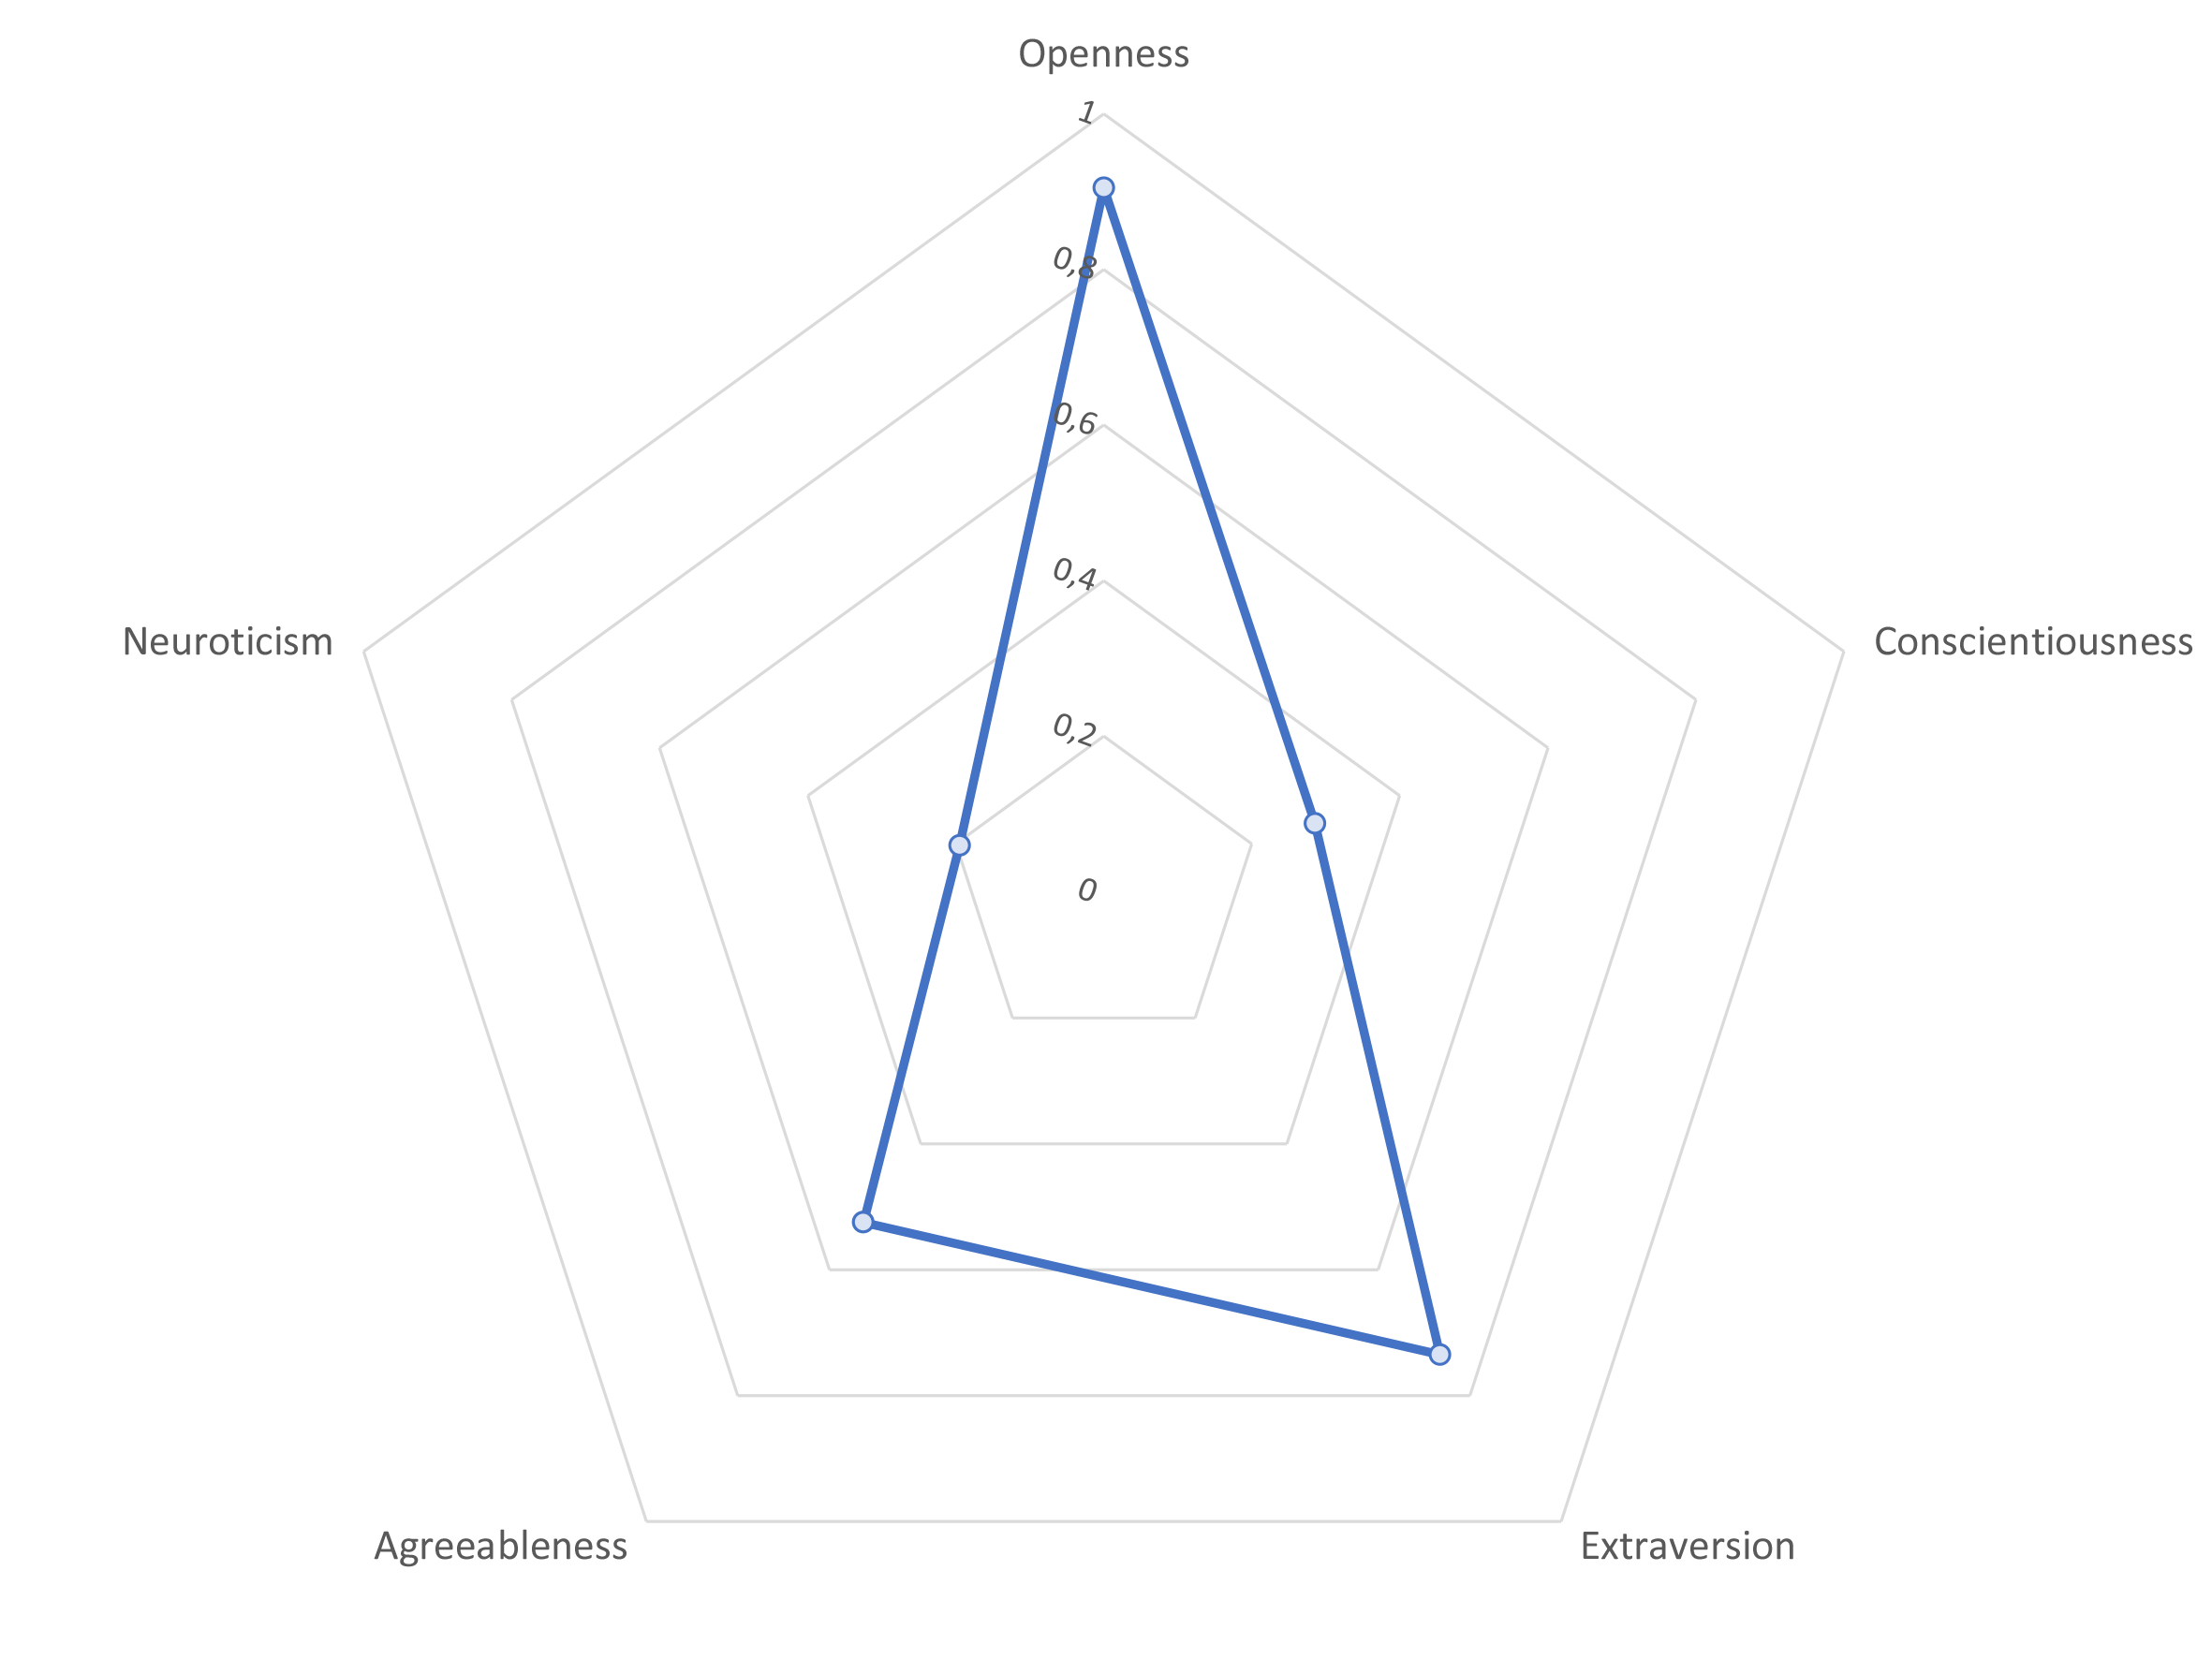
\includegraphics[scale=0.35]{figure/graph2_choleric}}
    \subfloat[Melancholic graph][Melancholic]{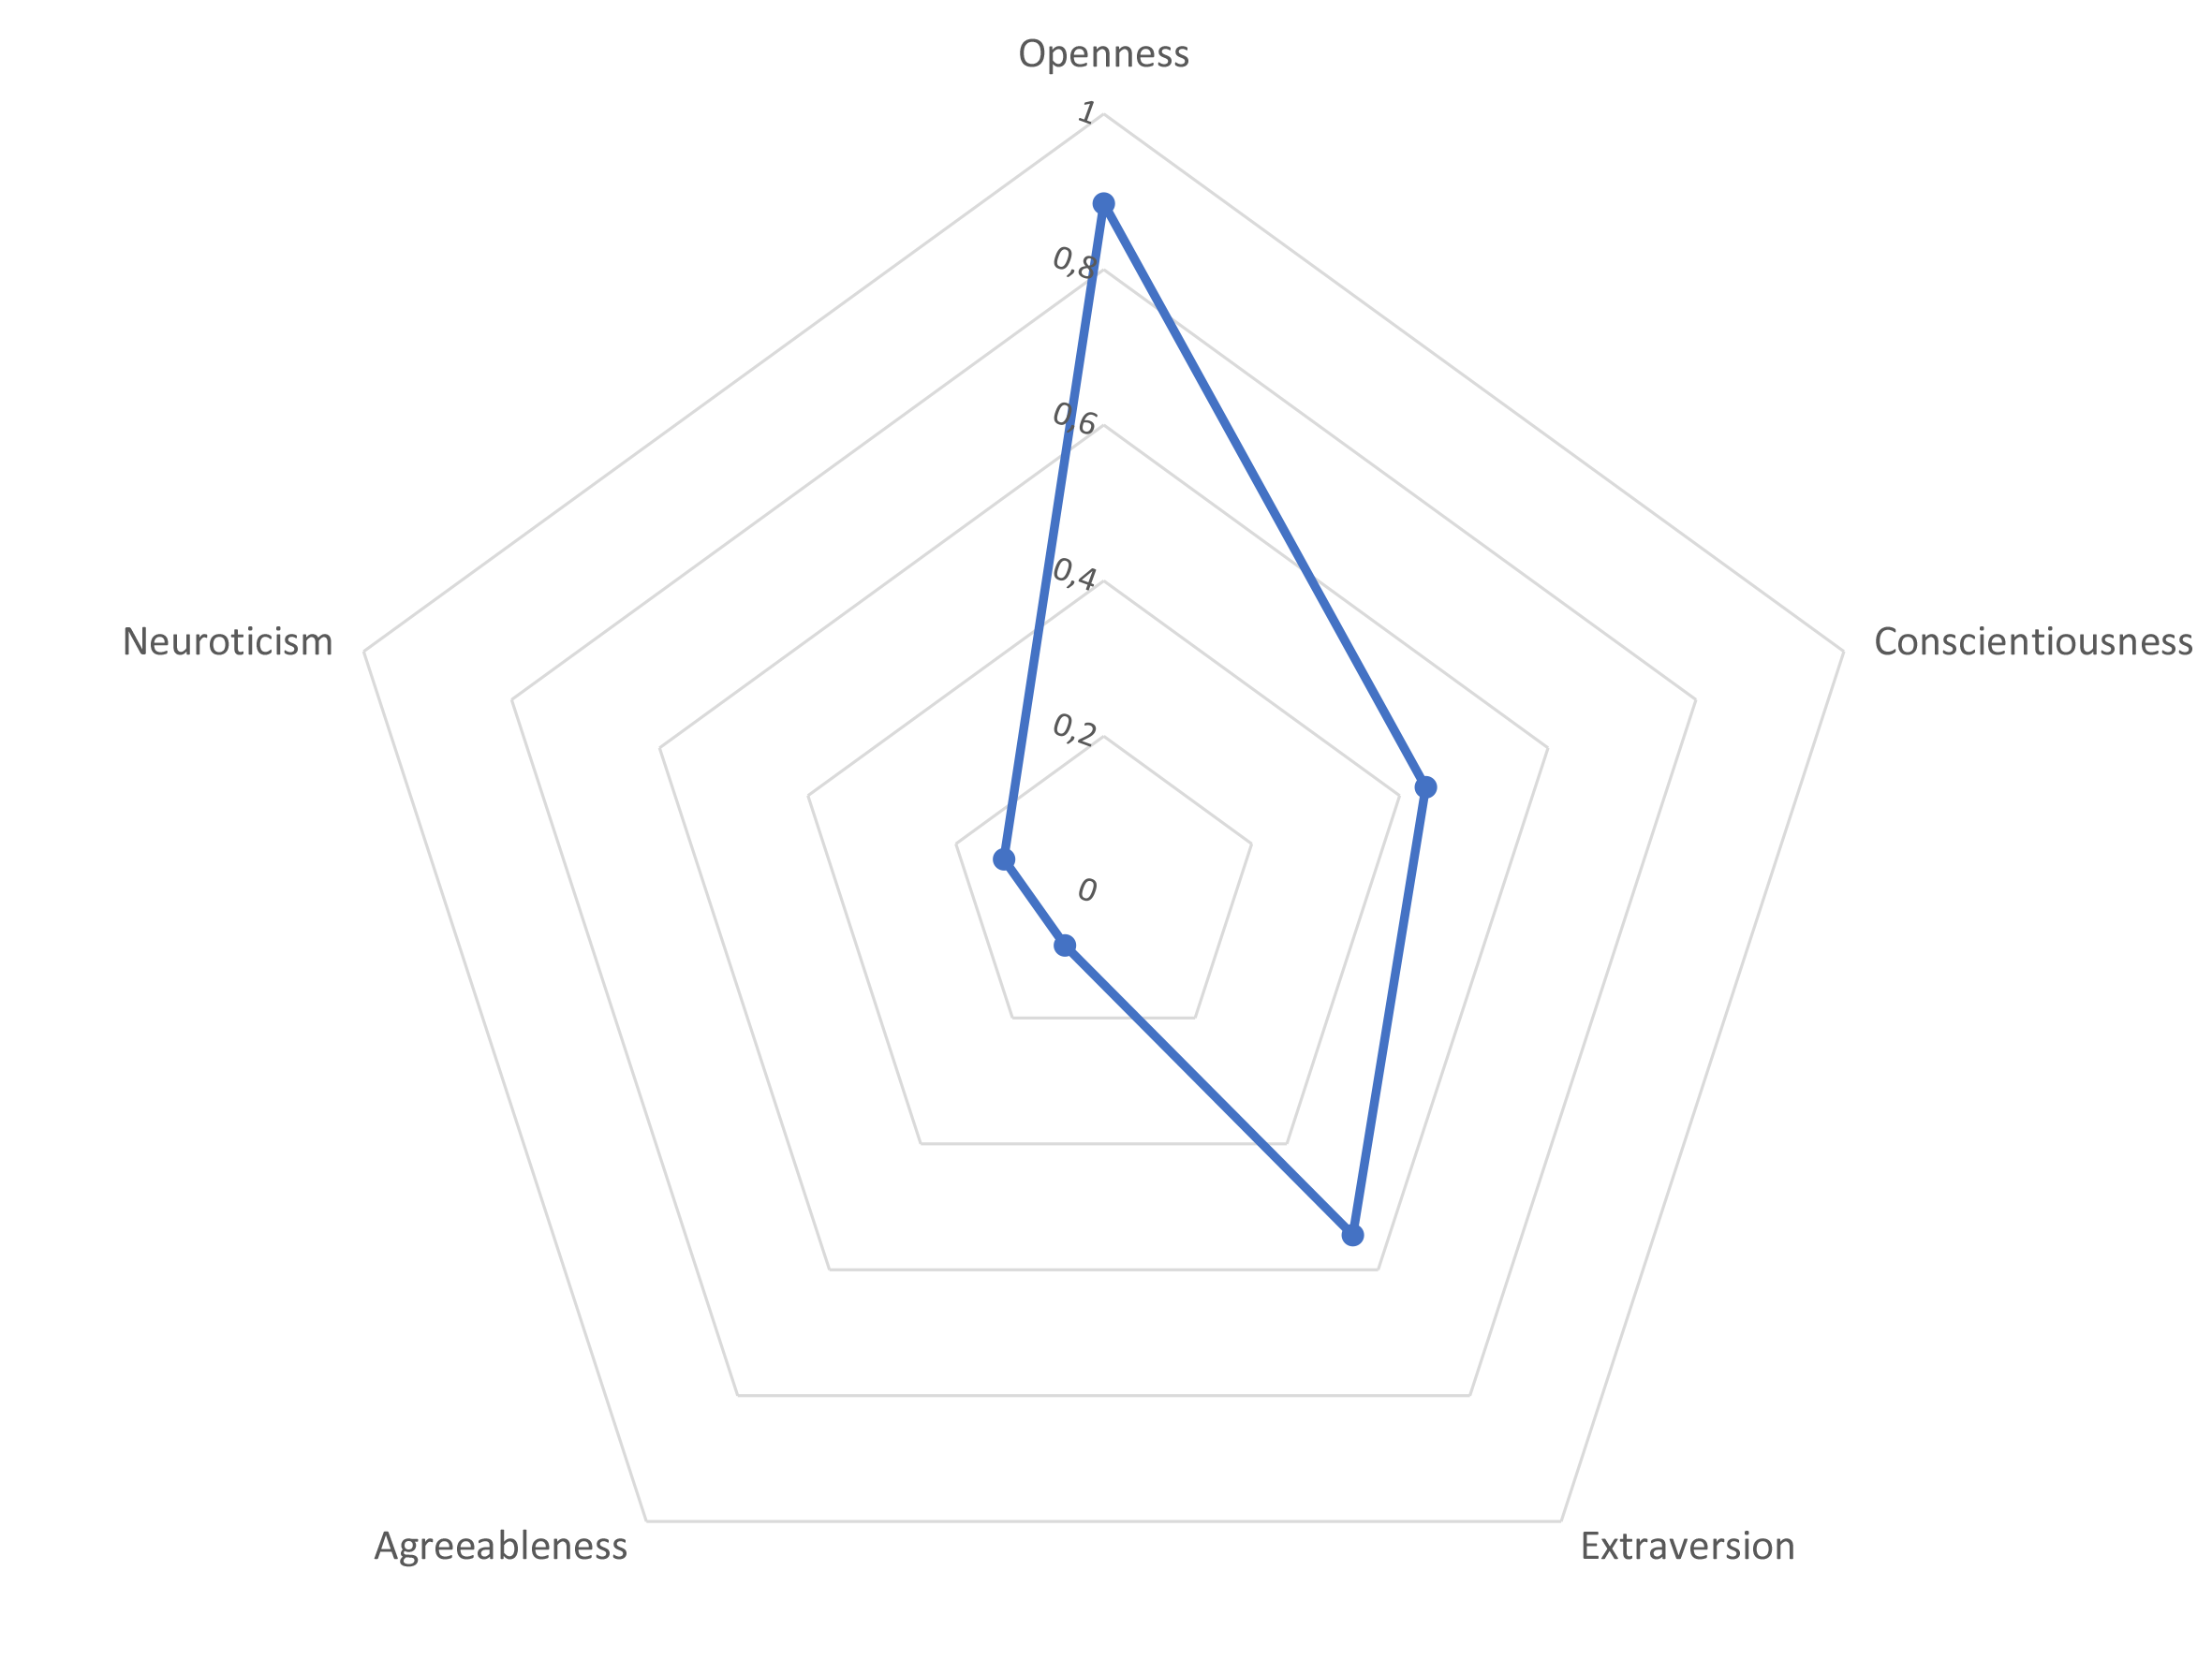
\includegraphics[scale=0.35]{figure/graph5_melancholic}}
    \qquad
    \subfloat[Sanguine graph][Sanguine]{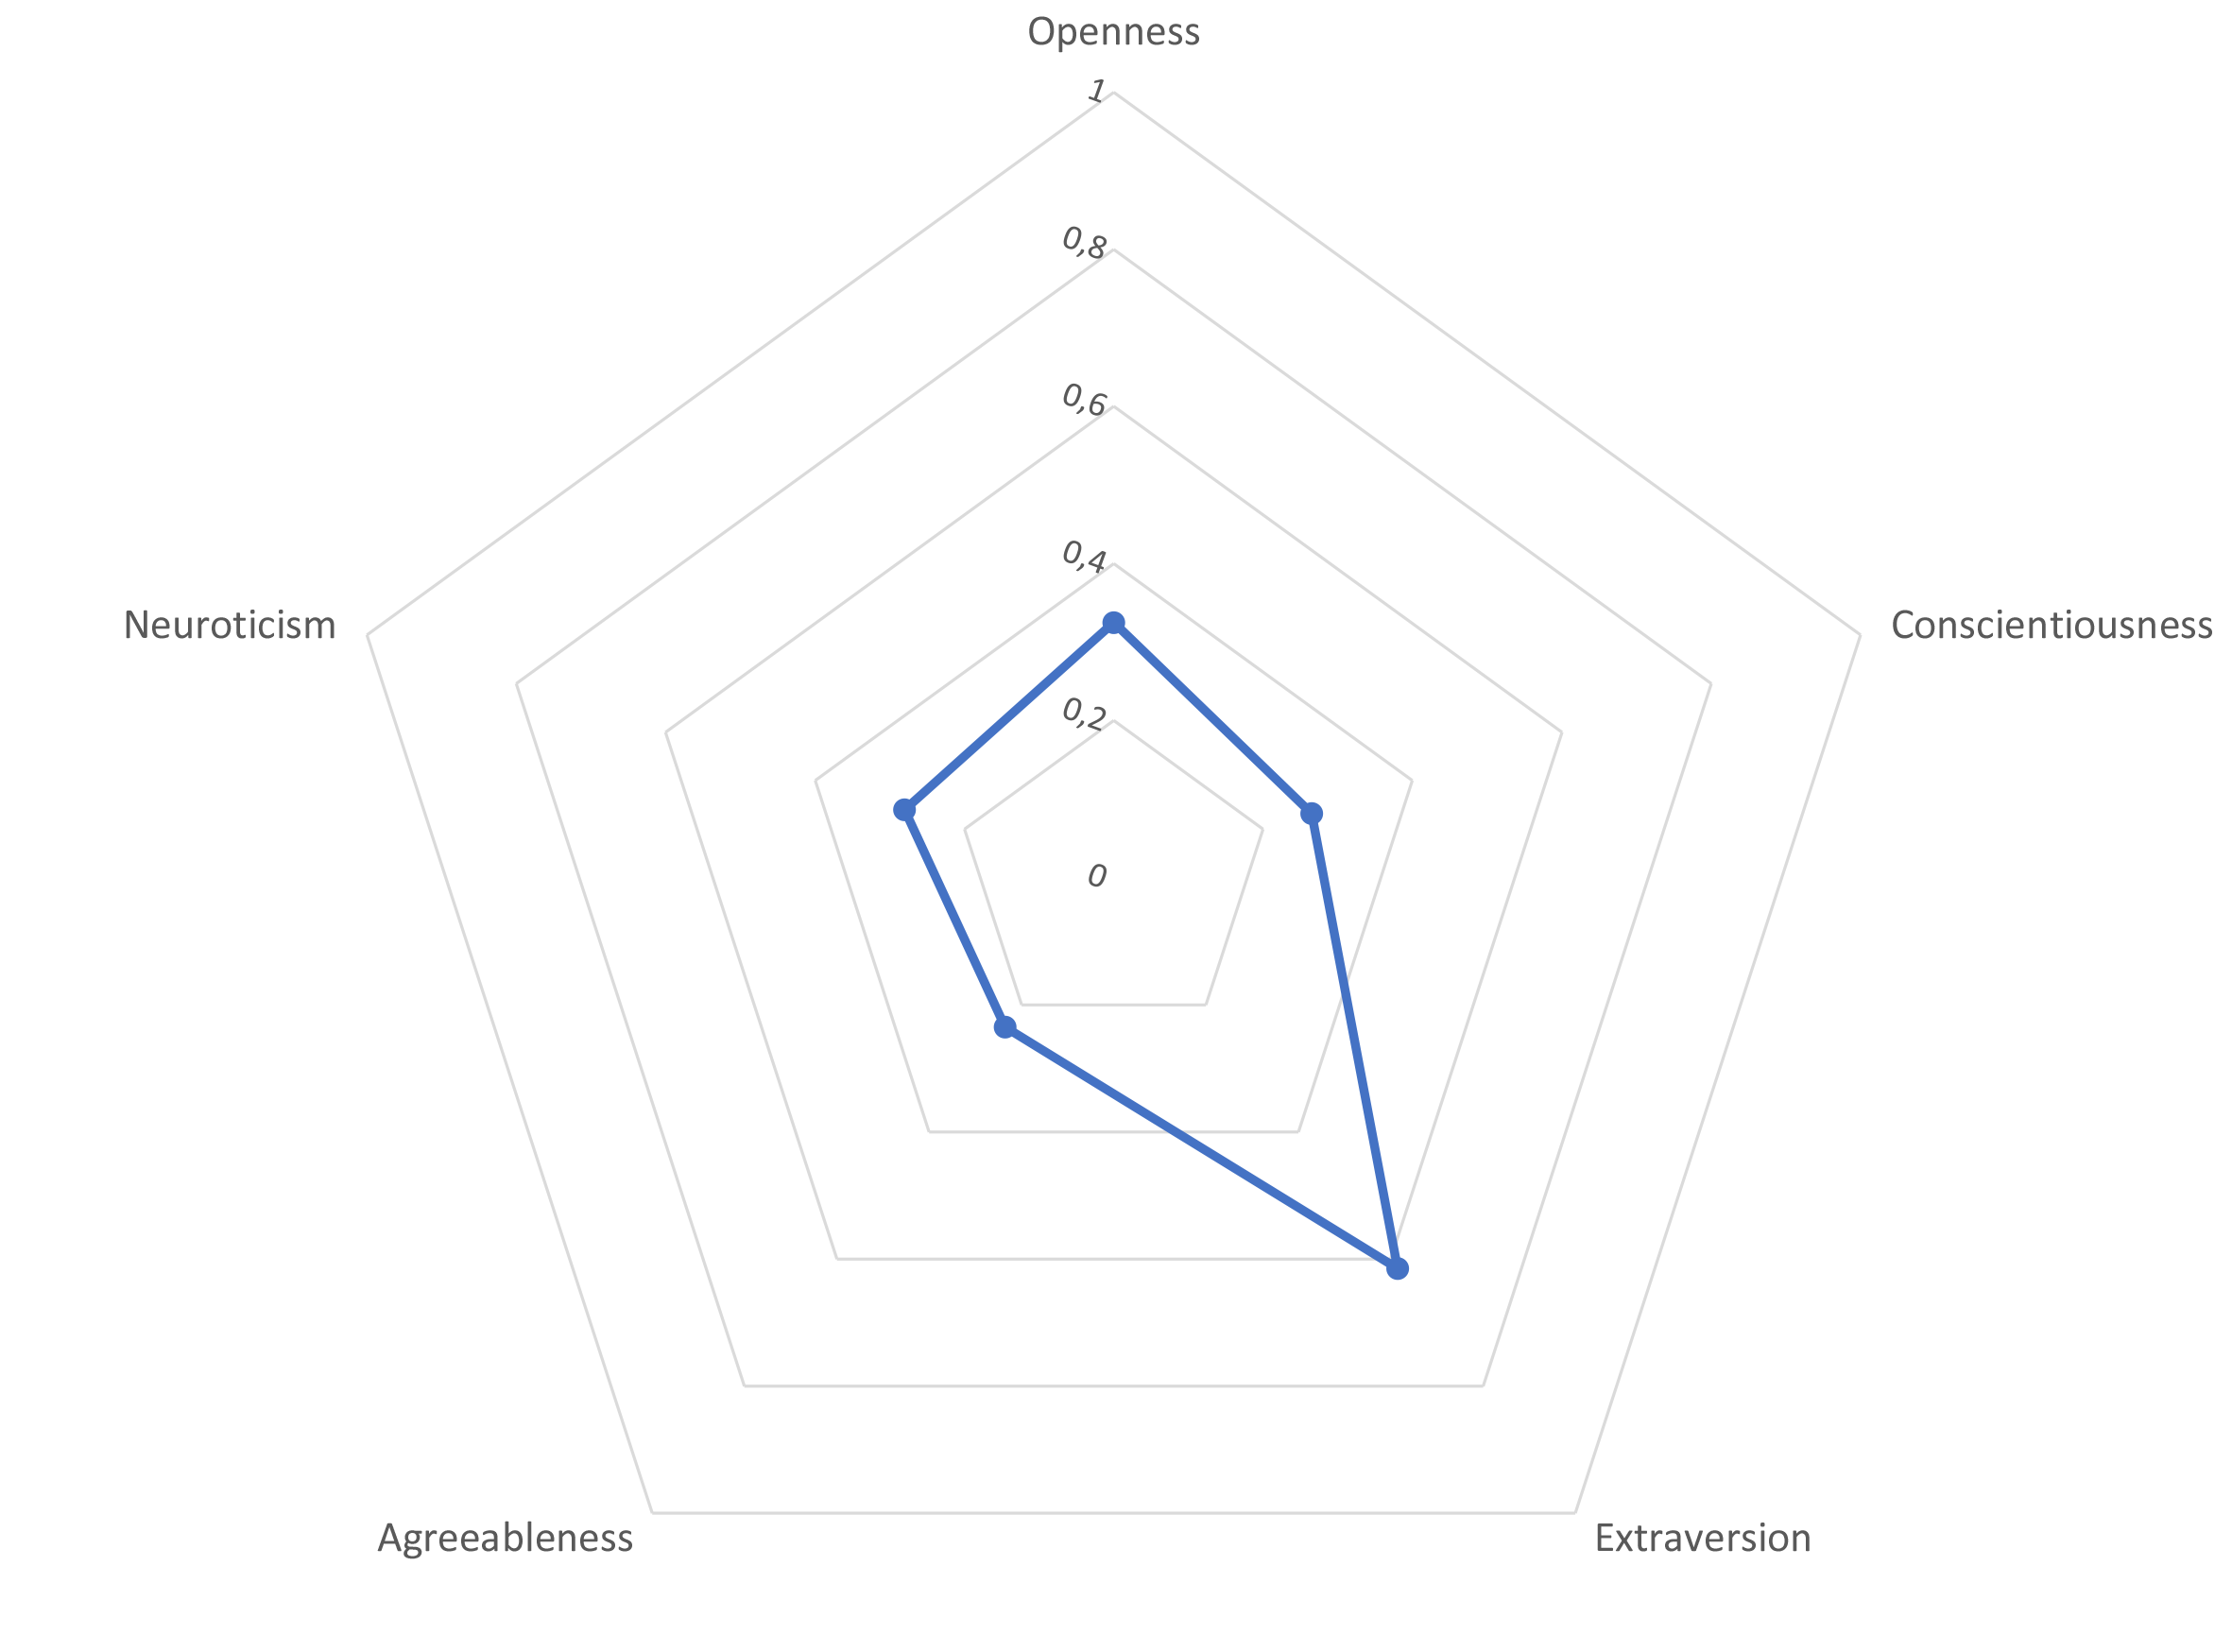
\includegraphics[scale=0.35]{figure/graph4_sanguine}}
    \subfloat[Phlegmatic graph][Phlegmatic]{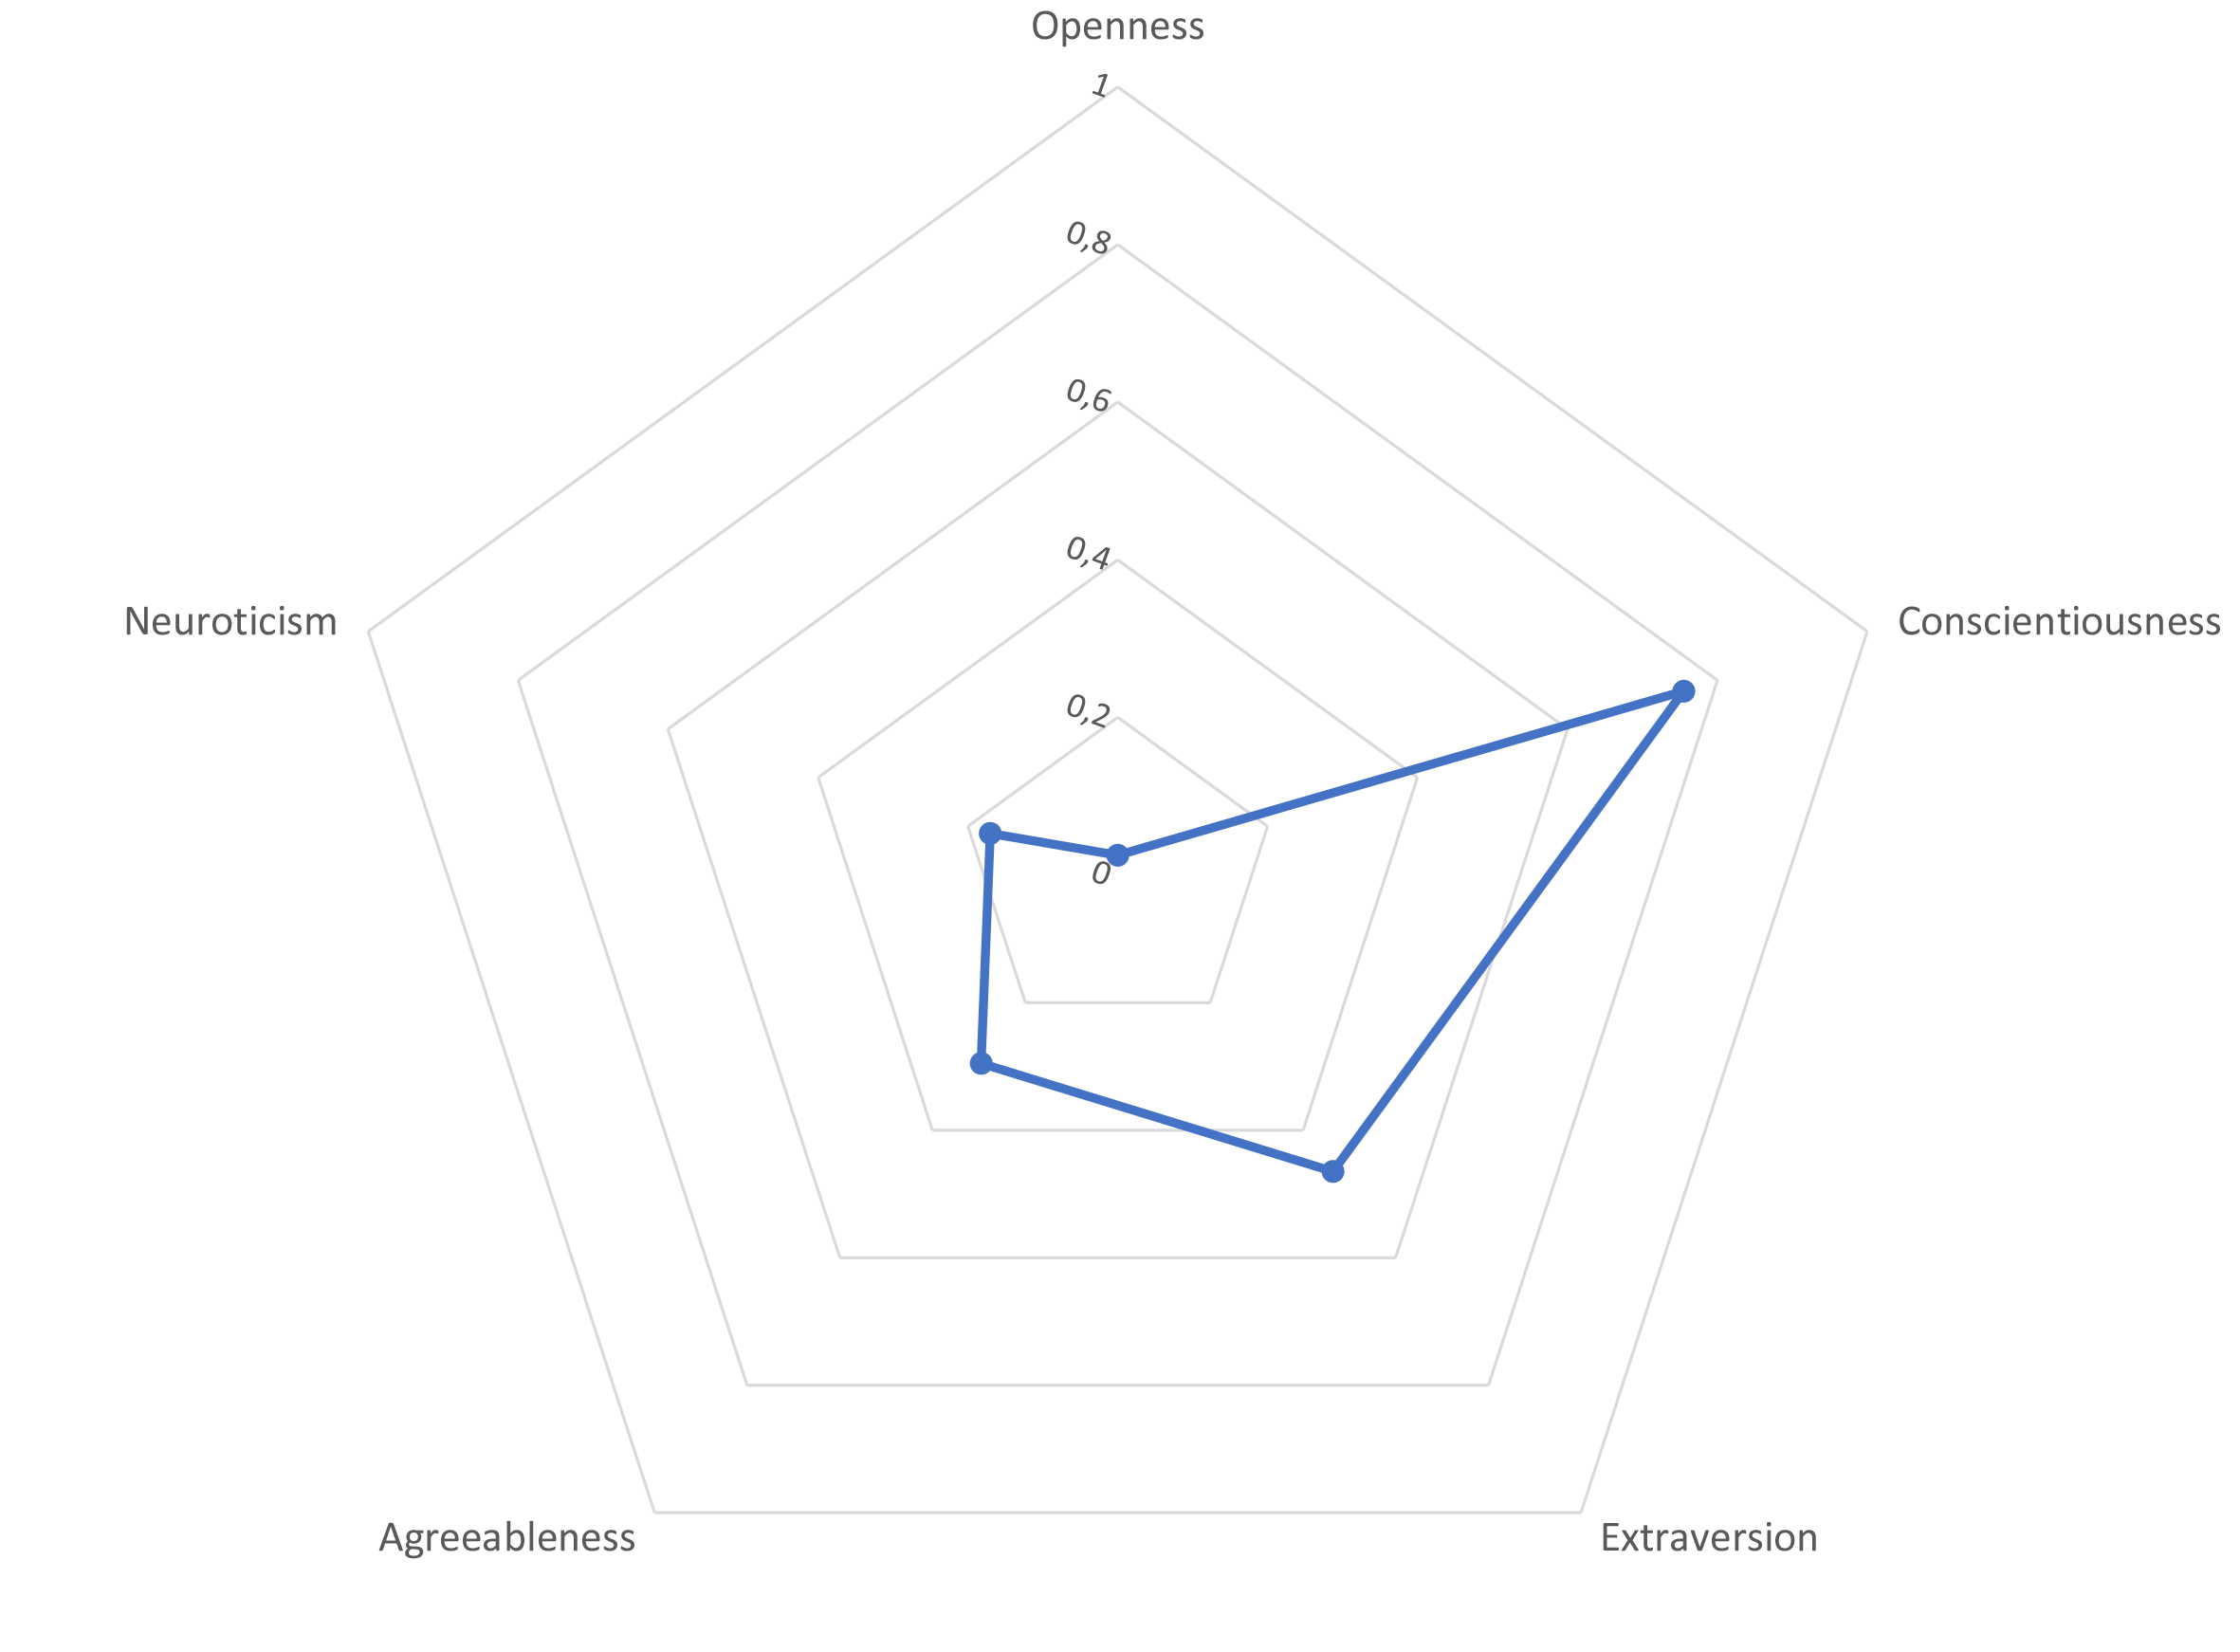
\includegraphics[scale=0.35]{figure/graph3_phlegmatic}}
  \captionsetup{justification=centering}
    \caption{The four graphs representing the correlation between each of the Four Temperaments and the factors that define the Big 5 model.}
    \label{fig:4t-big5}
\end{figure}
\section{Data Collection}\label{subsec:dataresults}
Trying to counterbalance the lack of user-friendliness of the Tiltyard server, and the time-consumption of some of the games that have been chosen, the data collection process has been ongoing from the beginning of this project to the very last weeks. However, once the data training had started, only the collection of Skirmish games was allowed, namely the matches required for the evaluation process.\\
Overall, data has been collected for 84 matches, in 46 different games, with 17 different users. The games involving two human players have been considered as two different matches for the genetic algorithm training, being associated to two different personalities and gaming styles. All users had different background and board games experience, and the most experienced players have been asked to try multiple games changing their playing style, trying to associate it to each of the different procedural personæ. Thanks to this, although the amount of games collected has been lower than expected, the distribution of games and personalities has been tendentially homogeneous in both personality and games distribution, as it can be seen from table \ref{tab:datac}.\\
\begin{table}[h]
    \caption{Summary of the games collected and the personality the users self-associated to themselves.}
    \centering
    \scriptsize
	\begin{tabular}{|c|c|c|c|c||c|}
    	\hline
					& Checkers & Skirmish & Connect Four & Nine Board Tic-Tac-Toe & Tot. \\
        \hline
        Melancholic & 1  & 3 & 4  & 17 & 25 \\
        \hline
        Choleric	& 5  & 1 & 8  & 8  & 22 \\
        \hline
        Phlegmatic	& 0  & 1 & 3  & 9  & 13 \\
        \hline
        Sanguine	& 4  & 3 & 11 & 6  & 23 \\
        \hline \hline
        Tot.		& 10 & 8 & 26 & 40 & 84 \\
        \hline
	\end{tabular}
    \label{tab:datac}
\end{table}
\noindent In the questionnaire given to the users, aside their own personality, they also have been asked to specify which personality they were perceiving from their opponent. Considering some bias toward the Phlegmatic personality due to Tiltyard's slow response, we can generally see a tendency in associating the opponents to the Melancholic and the Phlegmatic personalities, while the self-definition results in a more homogeneous spread. In table \ref{tab:datacpp} can be seen the summary of the perceived personalities of the opponents.\\
\begin{table}[h]
    \caption{Summary of the games collected and the perceived personality the users associated to their opponents.}
    \centering
    \scriptsize
	\begin{tabular}{|c|c|c|c|c||c|}
    	\hline
					& Checkers & Skirmish & Connect Four & Nine Board Tic-Tac-Toe & Tot. \\
        \hline
        Melancholic & 5  & 3 & 5  & 22 & 35 \\
        \hline
        Choleric	& 1  & 2 & 6  & 11  & 20 \\
        \hline
        Phlegmatic	& 4  & 2 & 10  & 5  & 20 \\
        \hline
        Sanguine	& 0  & 1 & 5 & 2  & 8 \\
        \hline \hline
        Tot.		& 10 & 8 & 26 & 40 & 84 \\
        \hline
	\end{tabular}
    \label{tab:datacpp}
\end{table}
As mentioned above, the Phlegmatic's numbers might be slightly skewed, inferring some false positive when the Tiltyard server was being unresponsive, and some false negative when the users realised that the long turns might have been caused by the system (ignoring completely - in such case - the possible phlegmatic tendency of the opponent). However, considering that a good part of our testers were in communication with each other - either in the same room, or in the IRC channel set up for them - we still think that, overall, the collected results could be meaningful. Nonetheless, this is the reason why only the self-described personality is taken into consideration for the training of our genetic algorithm.
It is interesting to see that among the 84 matches collected, in 16 of them (almost $20\%$) either of the players perceived the personality that was self defined by the opponent. The distribution of the success in matching the opponents personality can be found in table \ref{tab:matching}.
\begin{table}[h]
    \caption{Summary of the games where the users recognized successfully the opponent's personality.}
    \centering
    \scriptsize
	\begin{tabular}{|c|c|c|c|c||c|}
    	\hline
					& Checkers & Skirmish & Connect Four & Nine Board Tic-Tac-Toe & Tot. \\
        \hline
        Melancholic & 1 & 0 & 0 & 5  & 7 \\
        \hline
        Choleric	& 0 & 0 & 1 & 3  & 4 \\
        \hline
        Phlegmatic	& 0 & 1 & 2 & 1  & 3 \\
        \hline
        Sanguine	& 0 & 0 & 1 & 1  & 2 \\
        \hline \hline
        Tot.		& 1 & 1 & 4 & 10 & 16 \\
        \hline
	\end{tabular}
    \label{tab:matching}
\end{table}
Checkers and Skirmish were unknown games to most of the users before participating in the data collection, and that would excuse the inability to recognize any pattern, or strategy, in the opponent's game. Whilst Nine Boards Tic-Tac-Toe was a new game as well, the simple correlation to basic Tic-Tac-Toe, could have improved the process of following the gameplay. On the other hand, it can be assumed that the Melancholic type has been the most recognized as it might be easier to understand, by the end of the game, if the opponent has had a long term strategy ongoing during the whole match. 
\section{Genetic Algorithm}\label{sec:gares}
The Genetic Algorhtm has been executed a few times, over different sized sets of data, and the first thing to be noticed it  that the general fitness was much lower than it hoped for, causing the terminating test depending on acceptable fitness value $f_a=0.9$, to be unused. Only stagnancy of the individuals was then defining whether the algorithm would have terminated or not.\\


It has been mentioned in \ref{sec:ga} that a few test runs have been carried out in order to define which values to assign to the probabilities of crossover and mutation, $p_c$ and $p_{mut}$, and creep rate $C_r$. Those values have been tuned after several tests over the Phlegmatic's batch of games, which was the quickest to execute. The execution time of each block of games depended heavily on the games played, rather than on the parameters selection themselves. It is found that the Choleric and Sanguine batch, containing a higher number of Checkers games, are noticeably slower than the Phlegmatic group. In figure \ref{fig:runtimes} it can be seen how the Phlegmatic individuals have running time on the scale of $10^4ms$, while Choleric and Sanguine have it on the scale of $10^6ms$. The graphs also show how much impact the different parameters have on the execution times, which is generally consistent in the same personality data group, if we exclude a few noticeable peeks that reduce in number and intensity with the increasing of the generations. 
\begin{figure}[h]
\centering
    \subfloat[Choleric graph][Choleric] {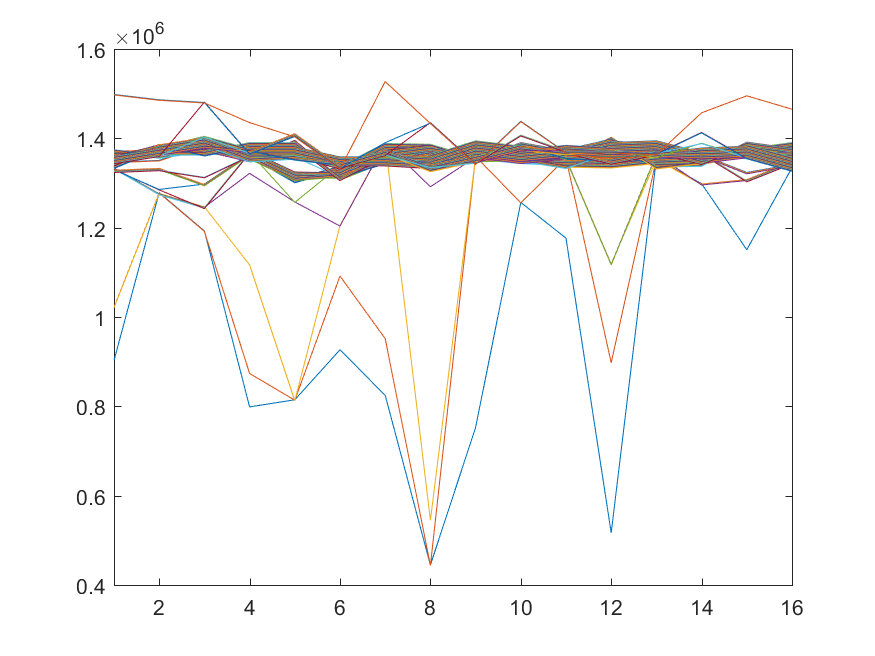
\includegraphics[scale=0.45]{figure/runtimeCh}}
    \subfloat[Melancholic graph][Melancholic]{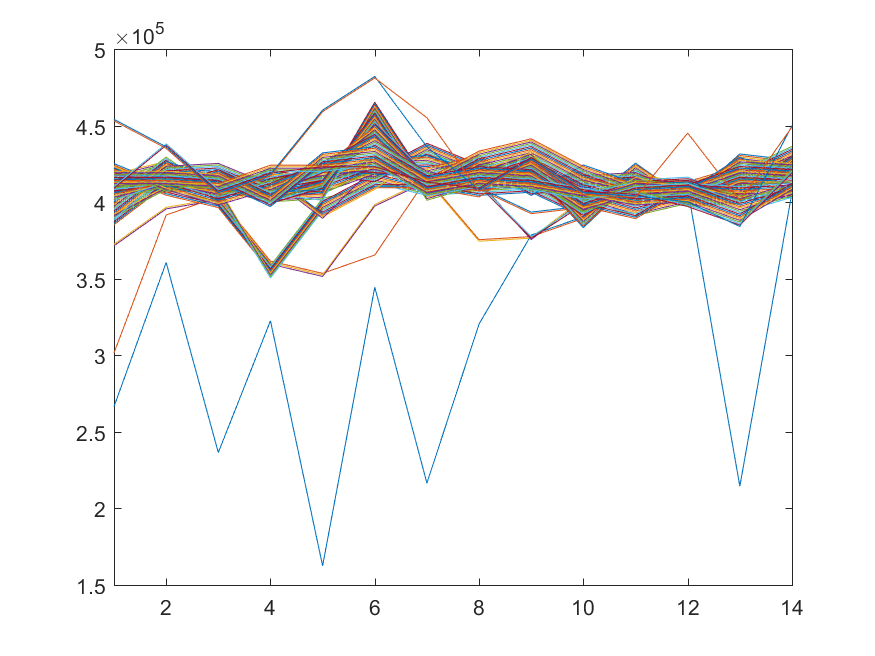
\includegraphics[scale=0.45]{figure/runtimeMe}}
    \qquad
    \subfloat[Sanguine graph][Sanguine]{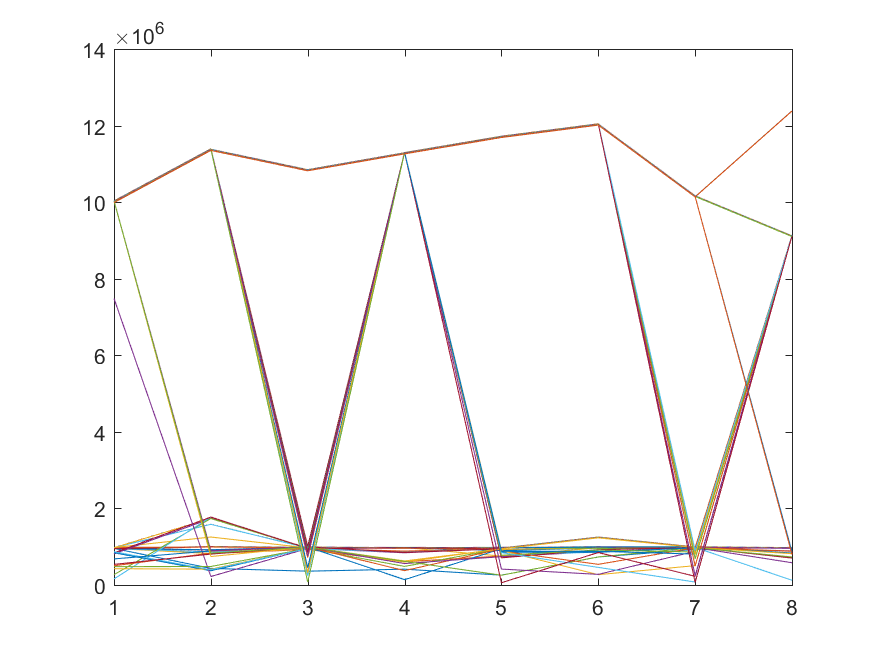
\includegraphics[scale=0.45]{figure/runtimeSa}}
    \subfloat[Phlegmatic graph][Phlegmatic]{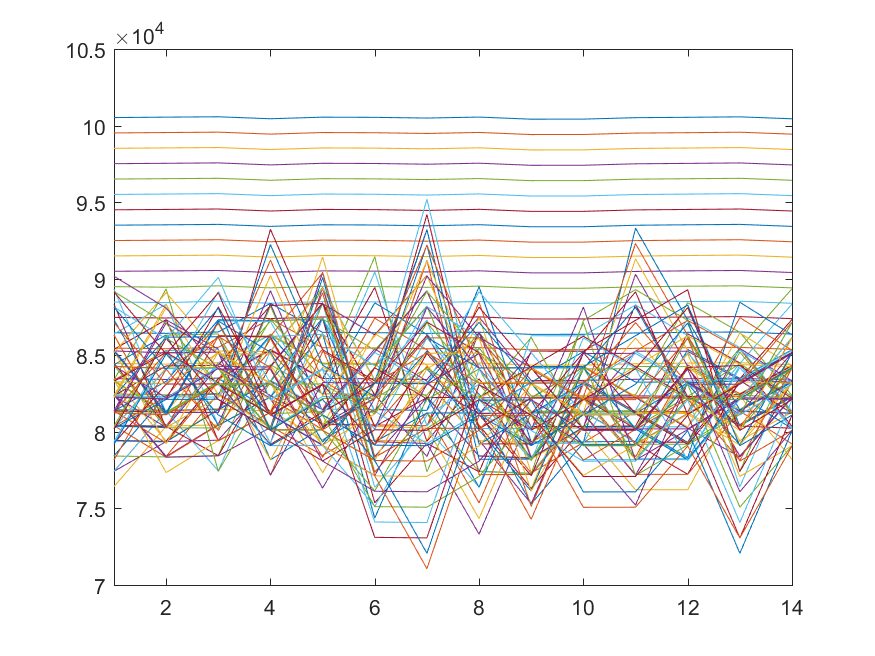
\includegraphics[scale=0.45]{figure/runtimePh}}
  \captionsetup{justification=centering}
    \caption{The four graphs represent the running times (in ms) for all the individuals in each generation, on y and x axis respectively.}
    \label{fig:runtimes}
\end{figure}

\subsection{Results Overview}
In Appendix \ref{sec:genegraphs} can be found the plots of the single individuals over three runs of the genetic algorithm. Each page contains the plots of the single genes, for each individual in each generation. Of those three runs, the first one has a different set of "algorithm" values $p_c$, $p_{mut}$, and $C_r$ than the ones described in section \ref{sec:ga}. Specifically, the first run adopts $p_c=0.8$, $p_{mut}=0.015$, and $C_r=0.2$. The first thing to be noticed from those plots is the number of generations. Although different "algorithm" values have been tested over a set of the data in order to maximise the number of generations - as mentioned earlier -, after the first tests, the results have become inconsistent. Several runs took long to stagnate (over 40 generations), whilst took other only few (8, for example). It has finally been decided to keep the same set of values, given the unpredictability of the number of evolutions.\\


It is to be noticed that different personalities tend to different values for the same gene. However, it is also to be pointed out that different runs aim at different results as well. That can be excused as the optimal individual that is picked does not look the same for each execution, leading to slightly different values combinations. Looking in more detail to some of the graphs in Appendix \ref{sec:genegraphs} it can be said that, when, for the each personality, different executions return very diverse values for the same parameter. What it means is that each parameter alone is not really relevant in the actions-matching for the personality in exam, as for example, the \emph{ChargeDefault} (see figure \ref{fig:phleChargeDef}). This statement can be clarified looking at figure \ref{fig:chargcorrl}. 
\begin{figure}[H]
\centering
    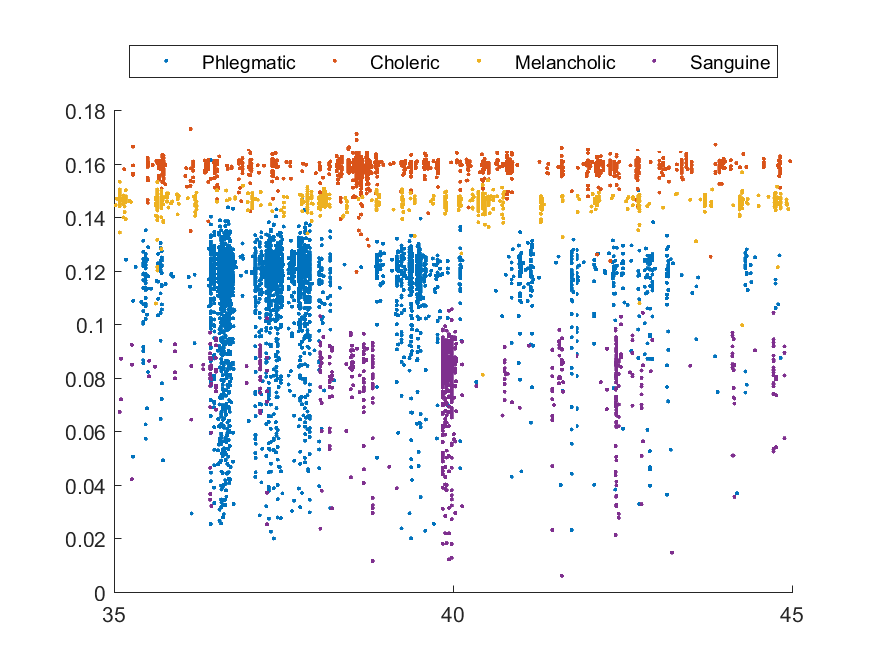
\includegraphics[scale=0.4]{figure/indfit/chargedeffit}
  \captionsetup{justification=centering}
    \caption{Correlation between specific Charge Default and fitness.}
    \label{fig:chargcorrl}
\end{figure}
It can be seen that each genes clusters around some specific values, however, not in a meaningful distribution. Further correlations need to be investigated, to understand which combination of parameters is indeed useful to influence the agent's game, and which are not.
\begin{figure}[ht!]	
\centering
    \subfloat[][Phlegmatic - I run]{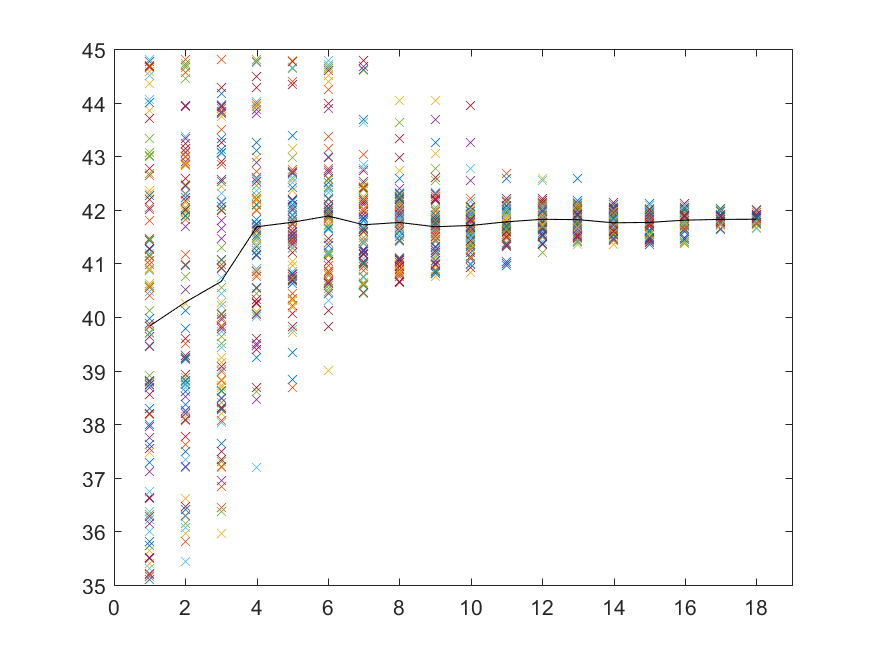
\includegraphics[scale=0.34]{figure/graphs1run/chargedefP}}
    \subfloat[][Phlegmatic - II run]{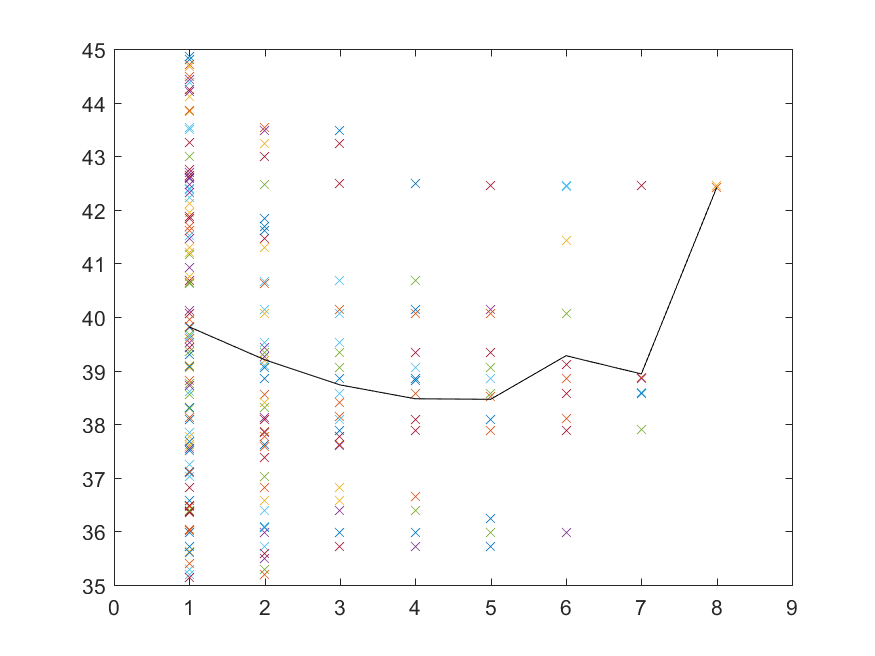
\includegraphics[scale=0.34]{figure/graphs2run/chargedefP}}
    \subfloat[][Phlegmatic - III run]{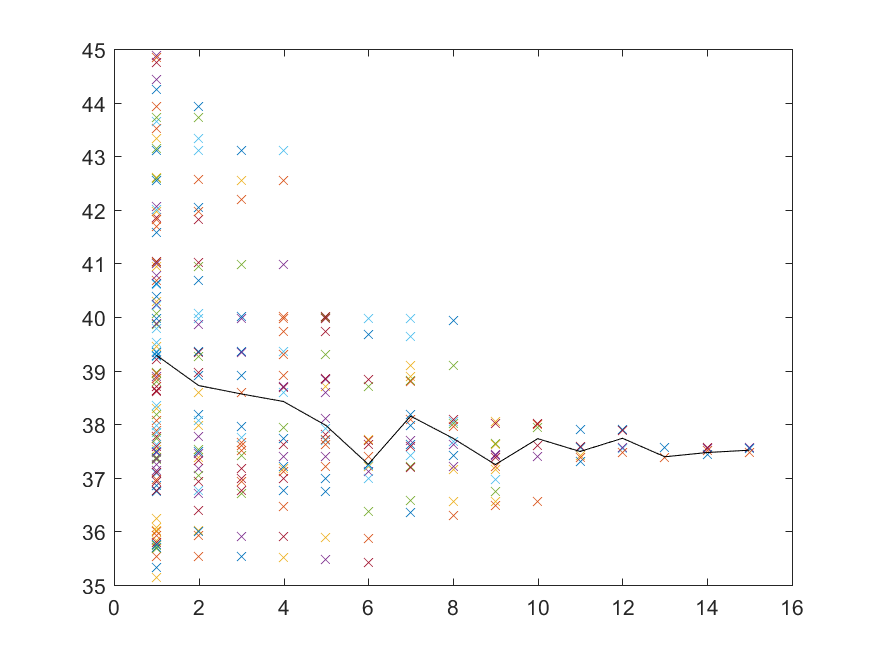
\includegraphics[scale=0.34]{figure/graphs3run/chargedefP}}
  \captionsetup{justification=centering}
  \caption{Charge Default gene for Phlegmatic personality.}
  \label{fig:phleChargeDef}
\end{figure}
It can also be noted from figure \ref{fig:explfact} that the \emph{Exploration Factor} gene seems to tend to the same value independently of the personality.\\
From the \emph{horizon} graphs in figure \ref{fig:horizon} it can be seen that the Melancholic type has generally a higher valued outcome, as it would be expected, being it the personality with the higher correlation to game strategy. In the same way, the parameter $NiceThreshold$ seems to generally be higher for Phlegmatic and Sanguine, and our model confirms them to be the two personalities with lower competitiveness. Figure \ref{fig:nicethresR} collects the results for the gene, after the third run.
\begin{figure}[ht!]
\centering
	\subfloat[][Choleric - III run] {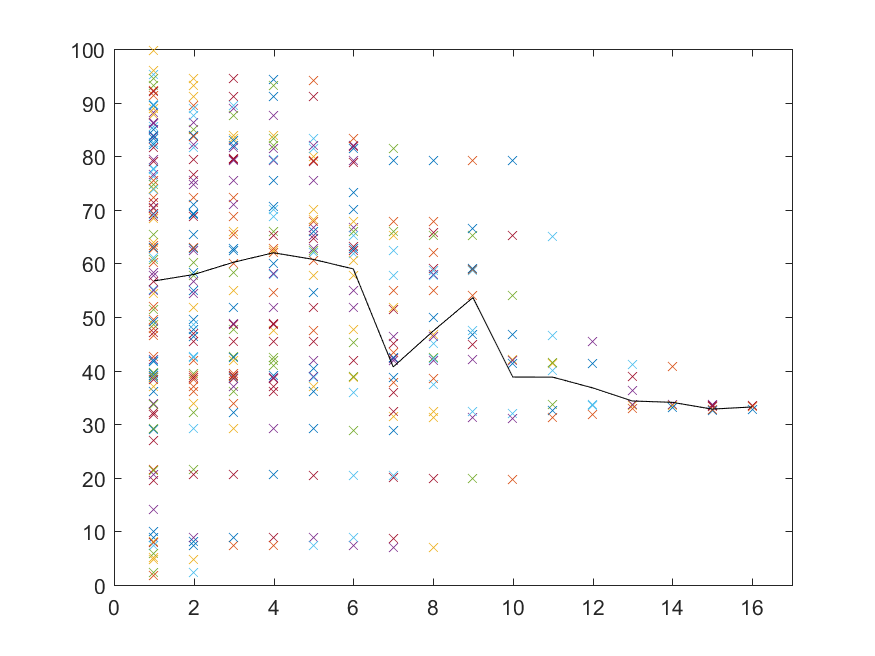
\includegraphics[scale=0.35]{figure/graphs3run/nicethresC}}
    \quad
    \subfloat[][Melancholic - III run]{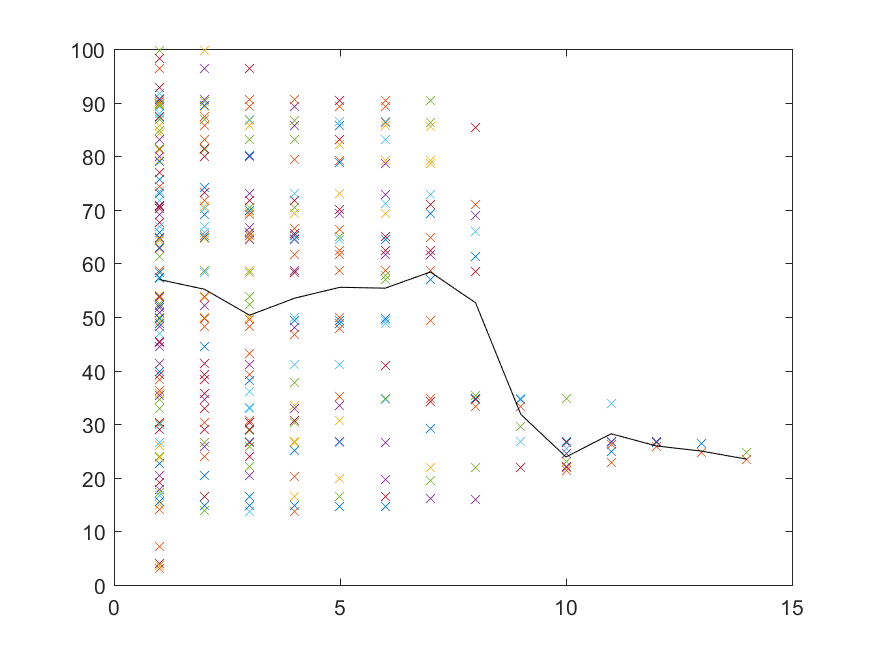
\includegraphics[scale=0.35]{figure/graphs3run/nicethresM}}
    \quad
    \subfloat[][Sanguine - III run]{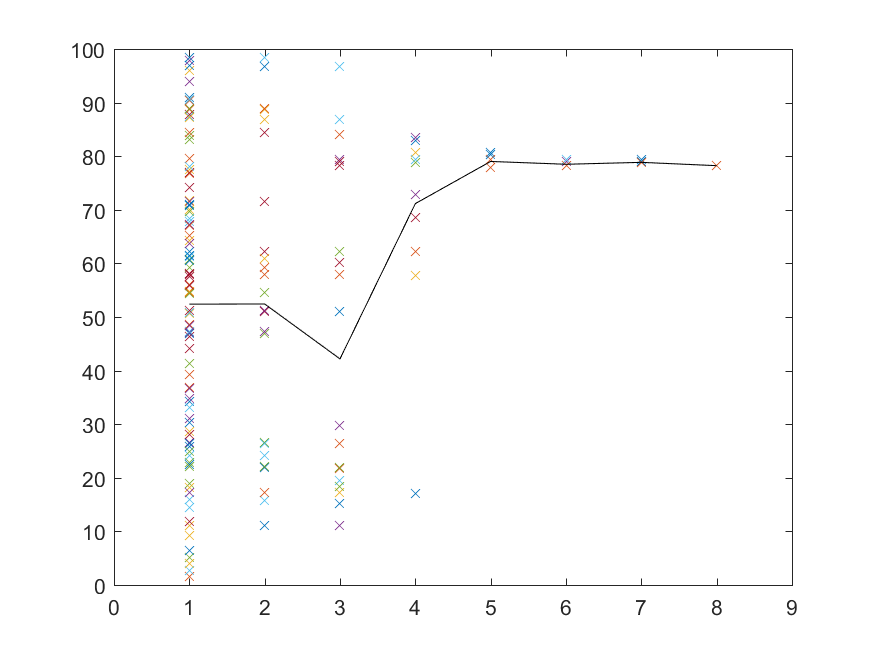
\includegraphics[scale=0.35]{figure/graphs3run/nicethresS}}
	\quad
    \subfloat[][Phlegmatic - III run]{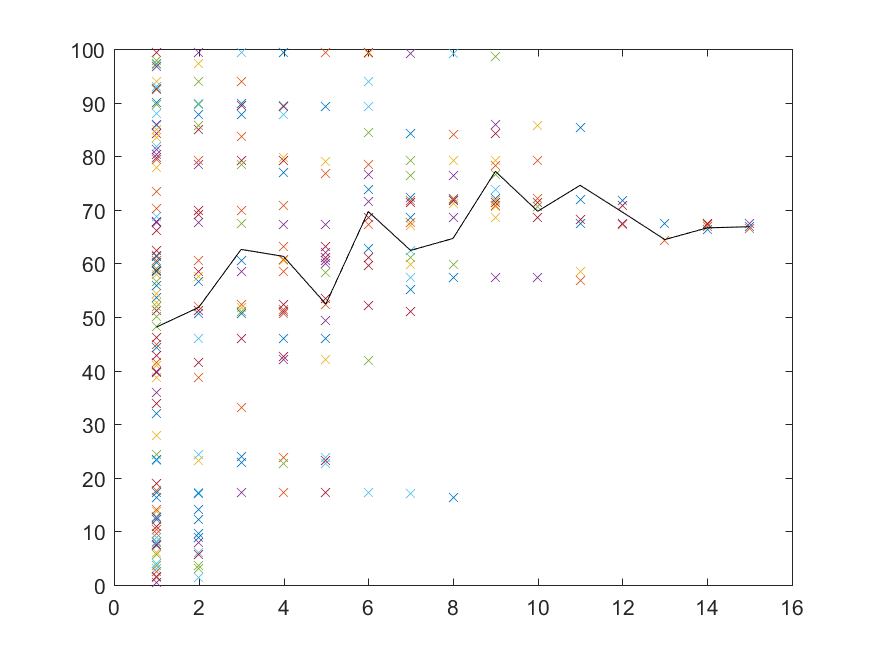
\includegraphics[scale=0.35]{figure/graphs3run/nicethresP}}
  \captionsetup{justification=centering}
    \caption{Nice Threshold gene's results of the III run.}
    \label{fig:nicethresR}
\end{figure}
Contrarily to our expectations, the \emph{RandomError} variable tends to a probability $P(RandomError)=0.5$, or higher in some cases (see figure \ref{fig:randomerrorR} for a clearer picture). We recall that this parameter controls the probability of picking a random move instead of the one suggested by the search. This means that half of the actions the MCTS outputs are aleatory, and that influences the fitness of the individuals, decreasing the helpfulness of elitism in keeping the individual with the highest fitness for the following generations.
\begin{figure}[h]
\centering
	\subfloat[][Choleric - III run] {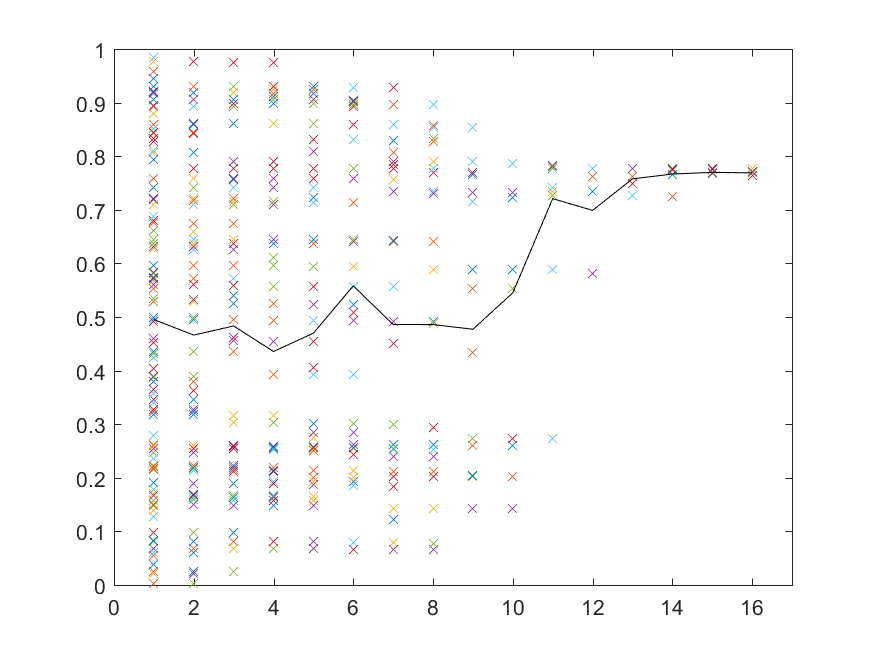
\includegraphics[scale=0.35]{figure/graphs3run/randomerrorC}}
    \quad
    \subfloat[][Melancholic - III run]{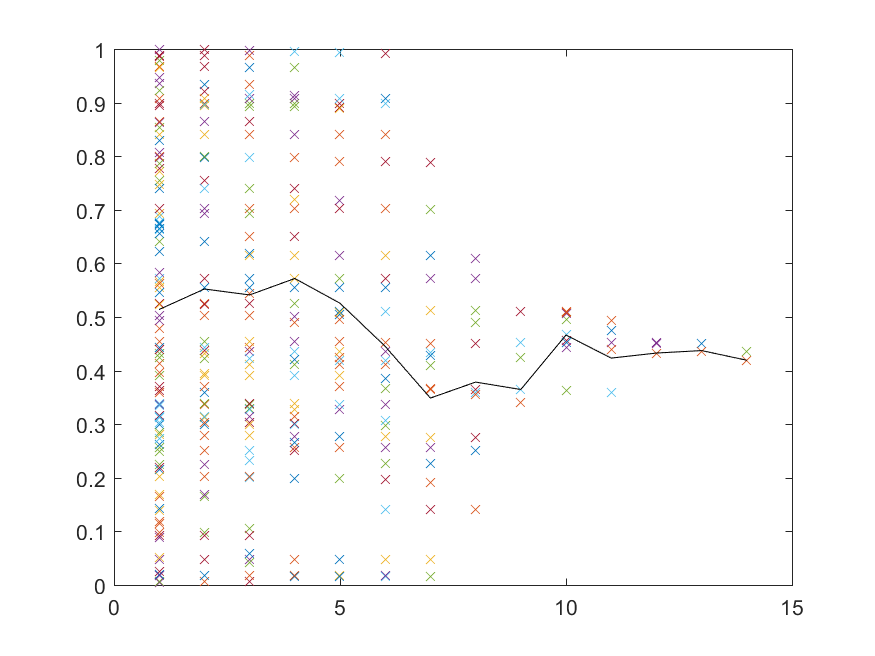
\includegraphics[scale=0.35]{figure/graphs3run/randomerrorM}}
     \quad
    \subfloat[][Sanguine - III run]{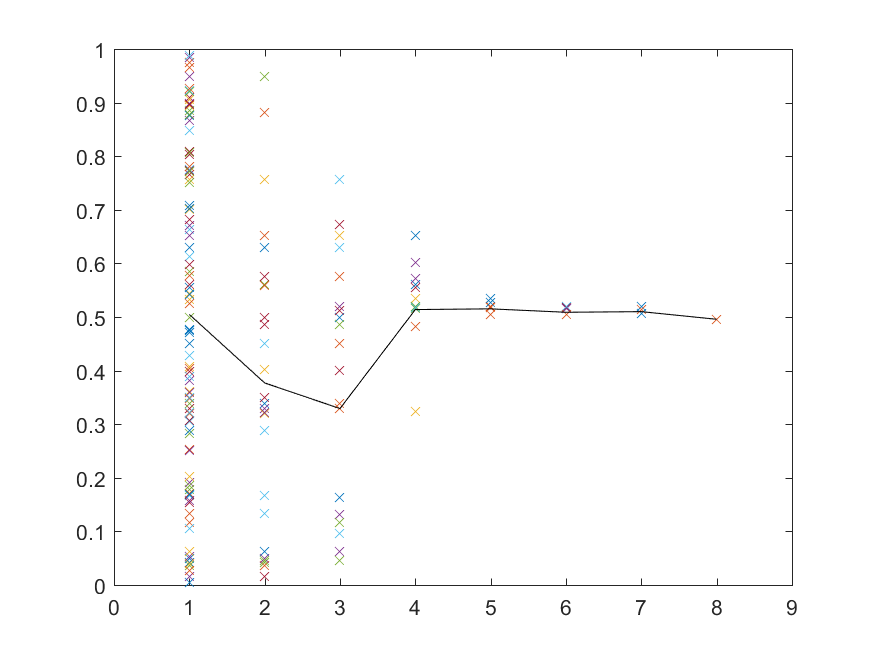
\includegraphics[scale=0.35]{figure/graphs3run/randomerrorS}}
	\quad
    \subfloat[][Phlegmatic - III run]{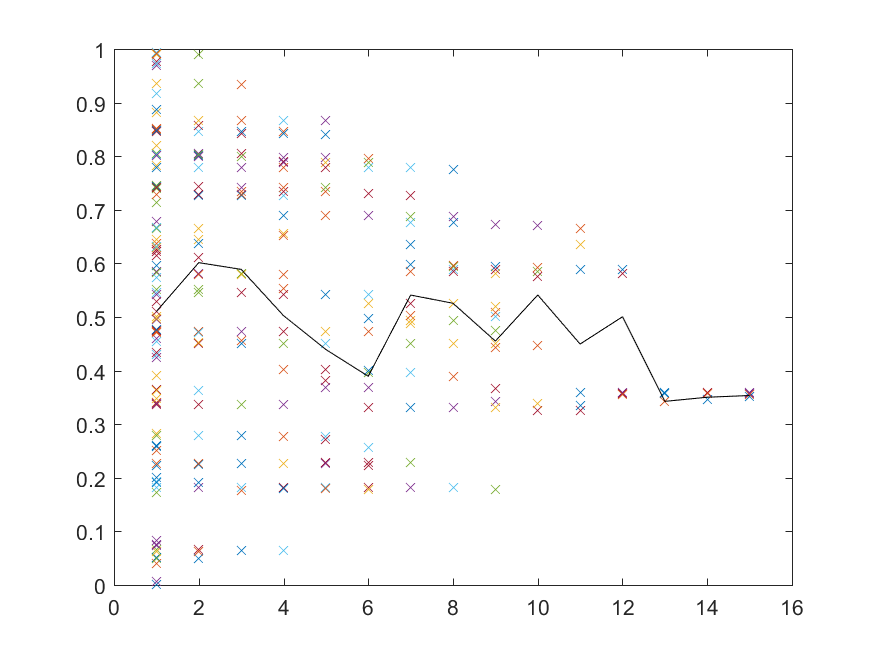
\includegraphics[scale=0.35]{figure/graphs3run/randomerrorP}}
  \captionsetup{justification=centering}
    \caption{Random Error gene's results of the III run.}
    \label{fig:randomerrorR}
\end{figure}
\subsection{Fittest Individuals}
After a few executions of the Genetic Algorithm, the fittest individuals for each of them have been picked to feed the evaluation process. The values are collected in table \ref{tab:fittest}. The Genetic Algorithm returns all doubles; the parameters are casted to the supposed type when plugged into the MCTS algorithm. The table aforementioned contains values that are partially already rounded (the ones with type \emph{long}, to be exact), while the floating point ones are rounded to the third decimal place.
\begin{table}[h]
	\caption{Fittest individuals picked for evaluation.}
    \centering
    \scriptsize
    \begin{tabular}{|c|c|c|c|c|}
    \hline
    Parameter & Phlegmatic & Sanguine & Choleric & Melancholic \\
        \hline
    epsilon & 0.264 & 0.507 & 0.435 & 0.045\\
        \hline
    rave & 2328 & 2744 & 4102 & 832\\
        \hline
    grave & 65 & 71 & 84 & 55\\
        \hline
    chargeDiscount &  0.937 & 0.947 & 0.985 & 0.930\\ 
        \hline
    treeDiscount & 0.952 & 0.943 & 0.972 & 0.969\\
        \hline
    aggression & 1.259 & 1.533 & 1.796 & 2.622\\ 
        \hline
    defensiveness & 1.161 & 1.878 & 0.208 & 0.725\\ 
        \hline
    chargeDepth & 53 & 54 & 47 & 61\\ 
        \hline
    horizon & 12 & 12 & 11 & 19\\
        \hline
    randErr & 0.503 & 0.451 & 0.398 & 0.380\\
        \hline
    chargeDefault & 41.768 & 40.014 & 39.984 & 35.782\\
        \hline
    explorationFactor & 68 & 81 & 71 & 105\\ 
        \hline
    niceThreshold & 33.903 & 55.308 & 24.593 & 12.885\\
        \hline
    \end{tabular}
    \label{tab:fittest}
\end{table}
In figure \ref{fig:fitnessfunc} can be seen the evolution of the fitness function, generation after generation. The red line represents the fitness of the fittest individual, calculated with equation (\ref{eq:fitnessfunc}); the blue line represents the average fitness of the individuals in that generation, while the blue errorbars are the standard deviation. Lastly, the black line represents the probability of picking a random move, referred here as "random-fitness". It was calculated as the geometric mean over all the matches of the probability $P(AnyMove)=\frac{1}{AvailableMoves}$ for each state. Considering that the MCTS is run always from the same state, it is expected that the probability $P(AnyMove)$ is constant throughout the generations. The optimal outcome would have been having the fitness of the fittest individual topping the random-fitness, but that is not true for most of the personalities. Figure \ref{fig:fitnessfunc} presents data from two different runs, as it is expected to be equally meaningful, the presented data has been chosen only on the basis of being clearer, although the results between executions are slightly different, they are equivalent nonetheless. 
\begin{figure}[ht!]
\centering
	\subfloat[][Choleric - III run] {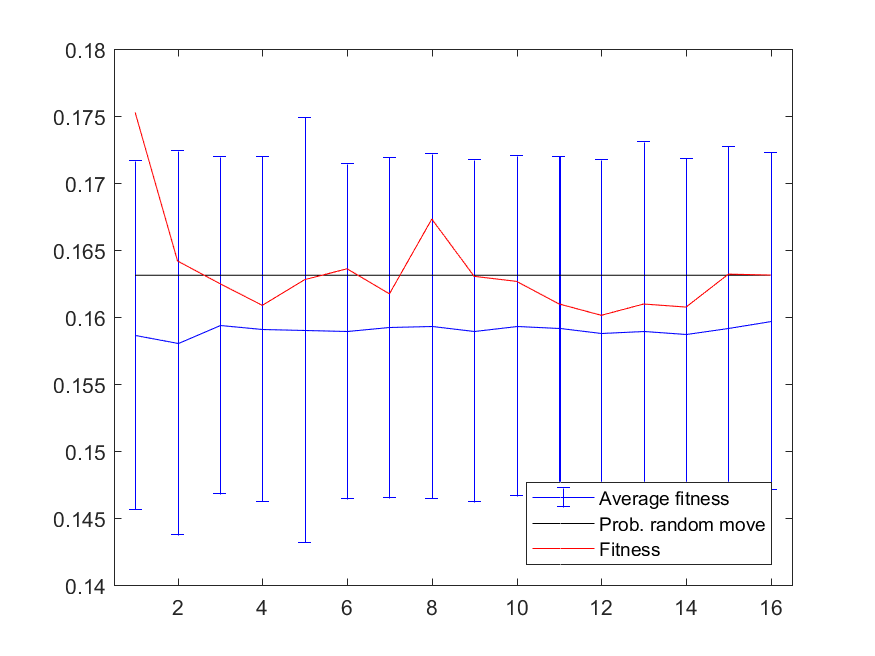
\includegraphics[scale=0.45]{figure/randCh}}
    \quad
    \subfloat[][Melancholic - IV run]{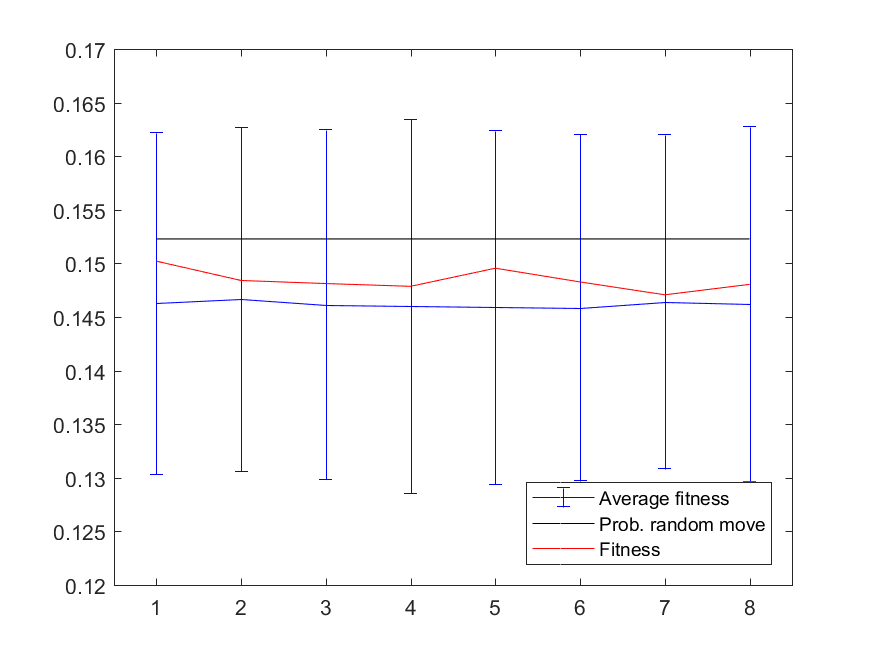
\includegraphics[scale=0.45]{figure/randMe}}
     \quad
    \subfloat[][Sanguine - IV run]{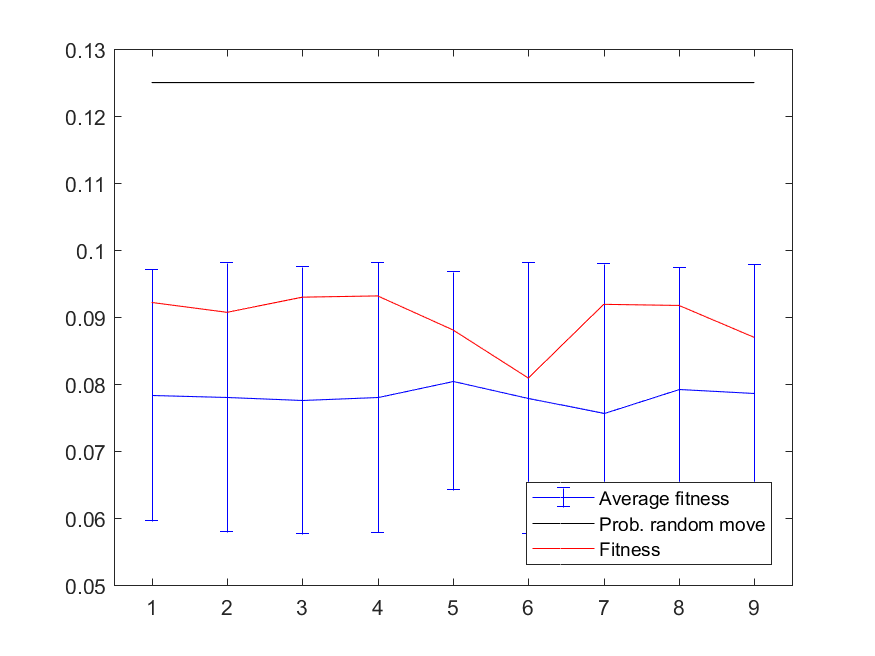
\includegraphics[scale=0.45]{figure/randSa}}
	\quad
    \subfloat[][Phlegmatic - III run]{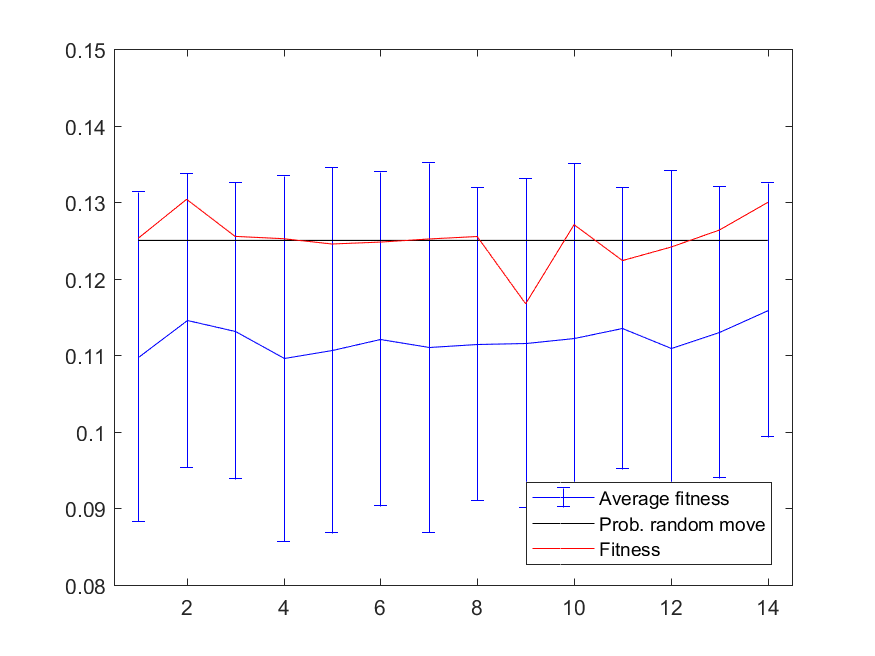
\includegraphics[scale=0.45]{figure/randPh}}
  \captionsetup{justification=centering}
    \caption{Fitness evolution throughout the generations, for each personality.}
    \label{fig:fitnessfunc}
\end{figure}
It is to be noted that, while the fittest individual is -averagely- not much better than only picking random moves at each turn, it is still above the average fitness among the individuals in the same generation, as expected.\\
For completeness, it is to be pointed out that only at report composing time it has been found a discrepancy between the geometric mean calculated by MATLAB (plotted in the graphs), and the one returned in the genetic algorithm logs. This is indeed a problem to be fixed, but considered the demanding computation required by the algorithm, it has been decided that this difference is irrelevant for the conclusions to be drawn.

\section{Results Game Play}\label{sec:reeval}
Among the games collected, only the Skirmish ones are used for evaluation purposes. Together with the skimming over the games recovered from the Tiltyard's bulks, it lead us to a total of 8 Skirmish games from the data collection and 54 games from the archives, divided in 22 Connect Four, 24 Nine Boards Tic-Tac-Toe, and 6 Checkers matches.
The evaluation algorithm has been running with the fittest individuals outputted by the genetic algorithm (see table \ref{tab:fittest}), and a set of random ones. The results are described below, while a selection of the gameplays' graphs can be found in appendix \ref{sec:genegraphs}.
\subsection{Skirmish Games with Fittest Individuals}
The first evaluation process has taken the fittest individuals resulting from the genetic algorithm. 
\begin{figure}[ht!]
\centering
	\subfloat[][Choleric] {\includegraphics[scale=0.45]{figure/eval/Skirmish/evalMatchskirCh1}}
    \quad
    \subfloat[][Melancholic]{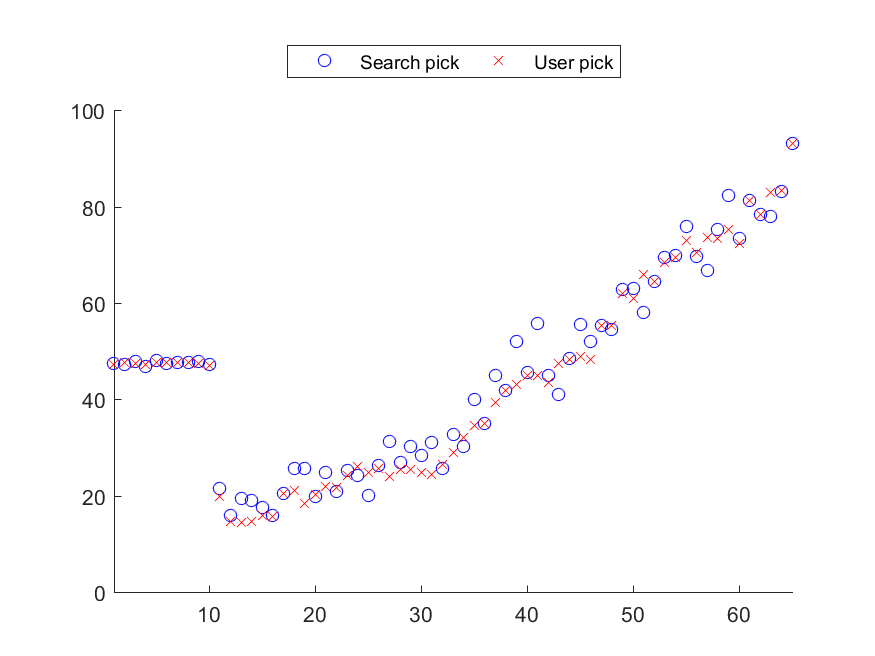
\includegraphics[scale=0.45]{figure/eval/Skirmish/evalMatchskirMe3}}
     \quad
    \subfloat[][Sanguine]{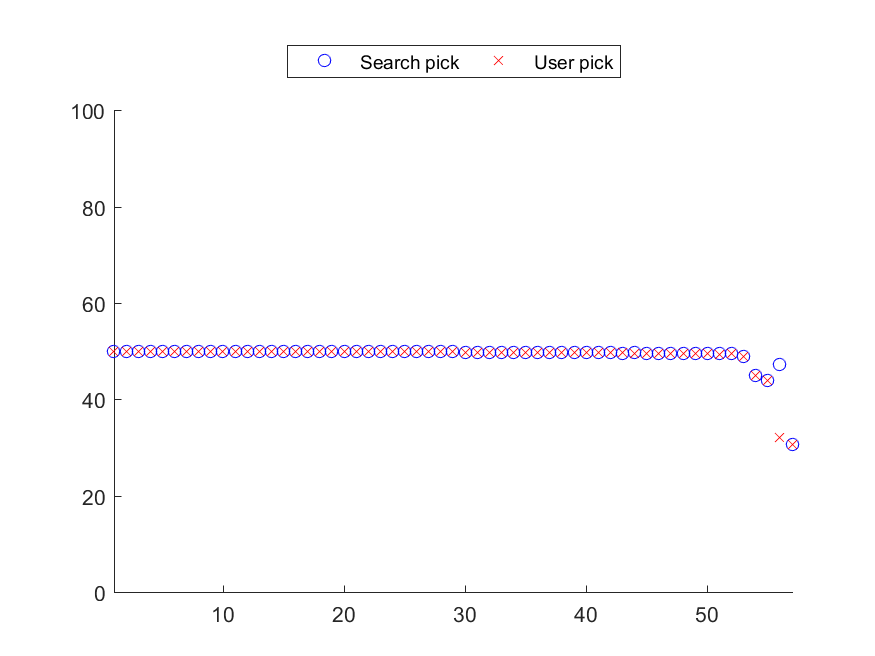
\includegraphics[scale=0.45]{figure/eval/Skirmish/evalMatchskirSa2}}
	\quad
    \subfloat[][Phlegmatic]{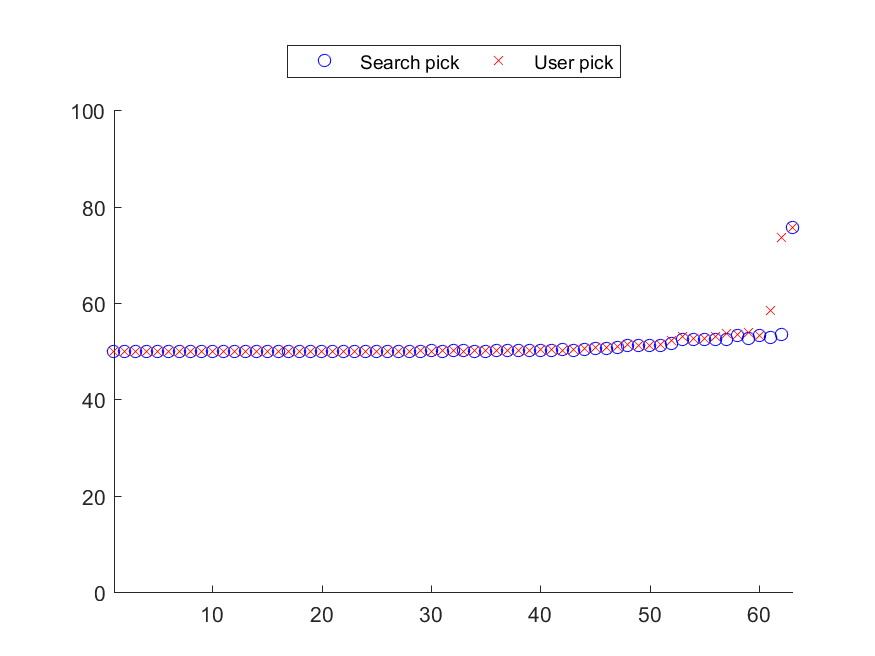
\includegraphics[scale=0.45]{figure/eval/Skirmish/evalMatchskirPh1}}
  \captionsetup{justification=centering}
    \caption{Evaluation of Skirmish matches.}
    \label{fig:skirmishE}
\end{figure}
Figure \ref{fig:skirmishE} shows the results of one Skirmish game for each personality, played with the "correct" parameters outputted by the GA. Although the logs confirm that search moves are not actually the same as the user's, figure \ref{fig:skirmishE} shows that the selected moves had an extremely similar QValue. It is necessary to point out that Skirmish is a game with a lot of legal moves at each state, averaging then the values of all of them. Table \ref{tab:cholski} contains the list of last moves in the Choleric game, to show that the actions selected are, as matter of fact, different, but essentially with the same weight.
\begin{table}[H]
	\caption{Last moves in the Choleric-Skirmish game.}
    \centering
    \scriptsize
    \begin{tabular}{|c|c|c|c|c|}
    \hline
    Search Action & QValue & User Action & QValue \\
        \hline
        {[( move 1 5 4 8 ), noop]} & 49.495 & {[( move 6 7 4 5 ), noop]} & 49.720\\
        {[noop, ( move 5 4 6 6 )]} & 49.791 & {[noop, ( move 5 4 4 6 )]} & 49.773\\
        {[( move 4 5 3 4 ), noop]} & 49.953 & {[( move 3 8 4 7 ), noop]} & 49.271\\
        {[noop, ( move 4 6 5 8 )]} & 49.217 & {[noop, ( move 4 6 6 5 )]} & 49.045\\
		{[( move 4 7 6 5 ), noop]} & 42.226 & {[( move 8 4 6 5 ), noop]} & 42.222\\
        {[noop, ( move 2 7 2 6 )]} & 39.652 & {[noop, ( move 2 7 2 5 )]} & 39.413\\
		{[( move 3 1 2 2 ), noop]} & 47.195 & {[( move 1 5 2 5 ), noop]} & 26.864\\
    \hline
    \end{tabular}
    \label{tab:cholski}
\end{table}
It is to be noticed that the Melancholic game seems to be the least moderate, however the search is still following pretty closely the trend set by the user.
\subsection{Random Games with Fittest Individuals}\label{sec:randGamesFitInd}
Plugging in the "correct" individuals in a set of games we have no knowledge about returned some interesting information. Appendix \ref{sec:genegraphs} contains plots of a few representative games, while here we would be describing only the most relevant ones.\\
\begin{figure}[ht!]
\centering
	\subfloat[][Sanguine - NBTTT - Match 2] {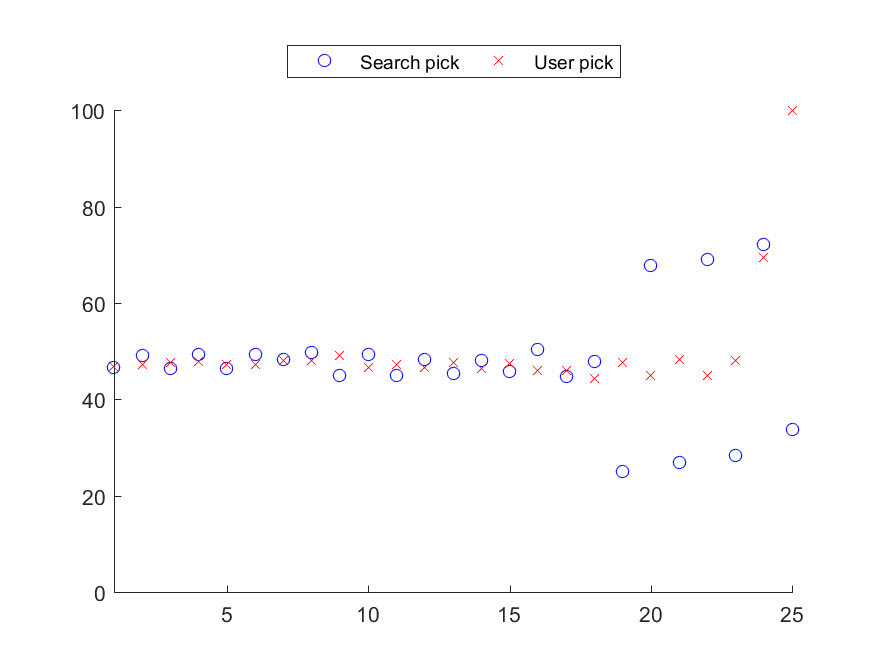
\includegraphics[scale=0.45]{figure/eval/TTTSa/evalMatchnbttt2}}
    \quad
    \subfloat[][Sanguine - NBTTT - Match 9]{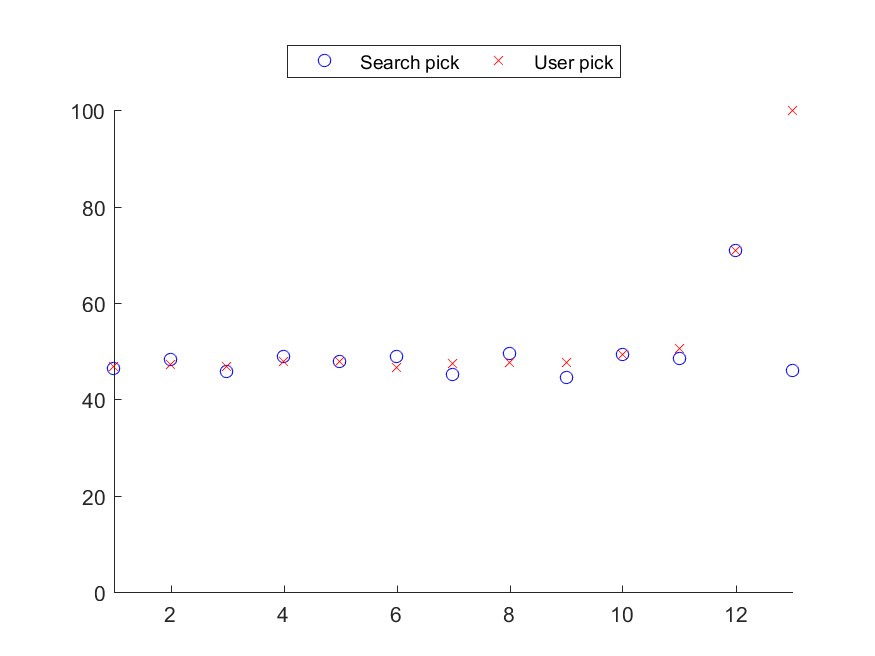
\includegraphics[scale=0.45]{figure/eval/TTTSa/evalMatchnbttt9}}
     \quad
    \subfloat[][Sanguine - NBTTT - Match 19]{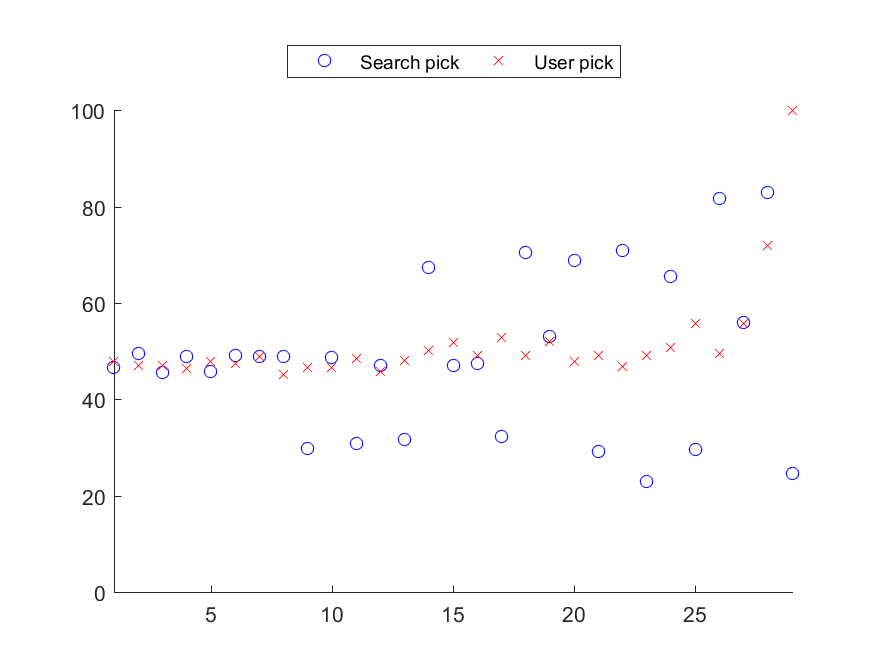
\includegraphics[scale=0.45]{figure/eval/TTTSa/evalMatchnbttt19}}
  \captionsetup{justification=centering}
    \caption{Evaluation of Nine Boards Tic-Tac-Toe for Sanguine personality.}
    \label{fig:nbtsa}
\end{figure}
In figure \ref{fig:nbtsa} can be seen three examples of tendency of game development, for the Sanguine personality, in games of Nine Boards Tic-Tac-Toe (NBTTT): figure (a) represents a mostly matching game, with divergence in the last states; figure (b) indicates more correlation between the search and the user's selection; finally, figure (c) shows a totally scattered selection. This can indeed mean that a few of those games were played by users with Sanguine personality, while others are related to other sets of parameters, therefore, another personality type.\\
Looking at the single matches, for both Nine Boards Tic-Tac-Toe and Connect Four, in figures \ref{fig:nbtttsa}, \ref{fig:nbtttph}, \ref{fig:nbtttme}, \ref{fig:nbtttch}, \ref{fig:c4sa}, \ref{fig:c4ph}, \ref{fig:c4me}, and \ref{fig:c4ch}, it can be noticed that Choleric and Sanguine tend to be a better fit. This implies that those two personalities might be easier to mimic, as well as that the personality model used in this thesis is not truly representative.\\
From figure \ref{fig:checkerseval}, presenting the results for the Checkers game, it can be seen that it has some of the Skirmish behaviour. Due to Checkers extensive state space, the difference in value between them is minimal. However, the Melancholic personality's search seems to have more difficulties matching the users', then the other personalities, confirming once more what said earlier about personalities that are easier to represent.
\begin{figure}[H]
\centering
	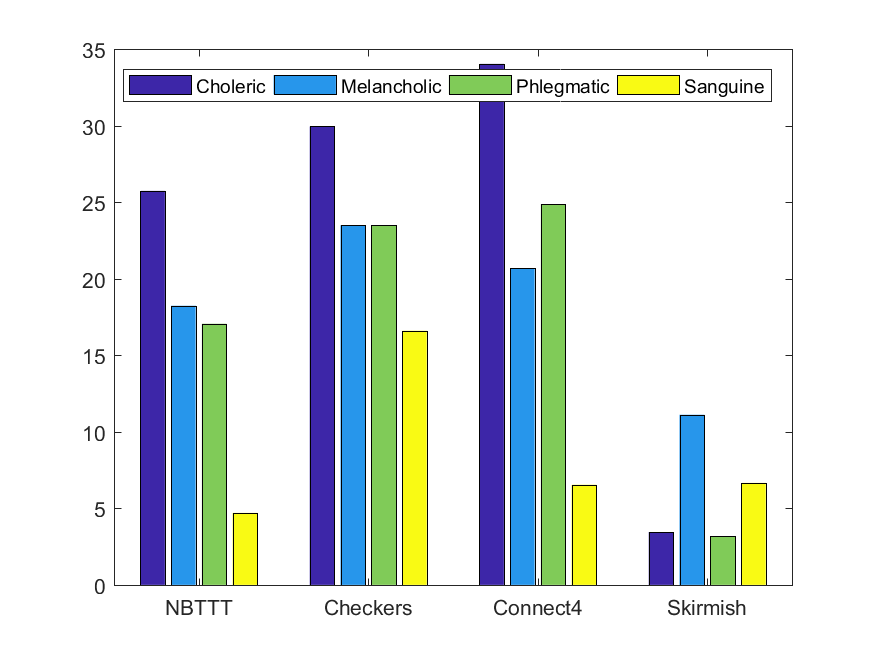
\includegraphics[scale=0.6]{figure/eval/Tot}
    \caption{Evaluation with Fittest Individuals (percent).}
    \label{fig:tot}
\end{figure}
Recapitulating, in figure \ref{fig:tot} is the summary of the Action Agreement Ratio for each game, once the search has been fed with the parameters from the genetic algorithm. It has to be pointed out that figure \ref{fig:tot} only includes the perfectly matching actions chosen by both the search and the users, while the graph in figure \ref{fig:skirmishE} only compares the moves' QValues. It is to be noticed that the Choleric parameters obtained from $25\%$ to $35\%$ matching moves, while Sanguine only $15\%$ in the best case. However, looking at figure \ref{fig:skirmishE}, it would look like more. That means that the actions chosen by the search is extremely similar in QValue to the one picked by the human player. Therefore, that might imply that the choice between the two moves is equivalent, and still achieve a human-like gaming style. 
\subsection{Skirmish Games with Random Individuals}\label{sec:skirmishrandom}
The skirmish games that had been collected, and associated to a personality, have also been tested with 3 random sets of parameters. In figure \ref{fig:randomSkirmish} is an extract of the graphs collected, showing how the behaviour of the search changes, on the same match, depending on the parameters plugged in. We found irrelevant to show the graphs relative the rest of the matches for Melancholic and Sanguine, as the behaviour is tendentiously the same as the one showed in figure \ref{fig:randomSkirmish}.
\begin{figure}[h]
\centering
    \subfloat[][Choleric Match 1 - Random Individual 1] {\includegraphics[scale=0.35]{figure/eval/rand/evalMatchskirCh1}}
    \subfloat[][Choleric Match 1 - Random Individual 2] {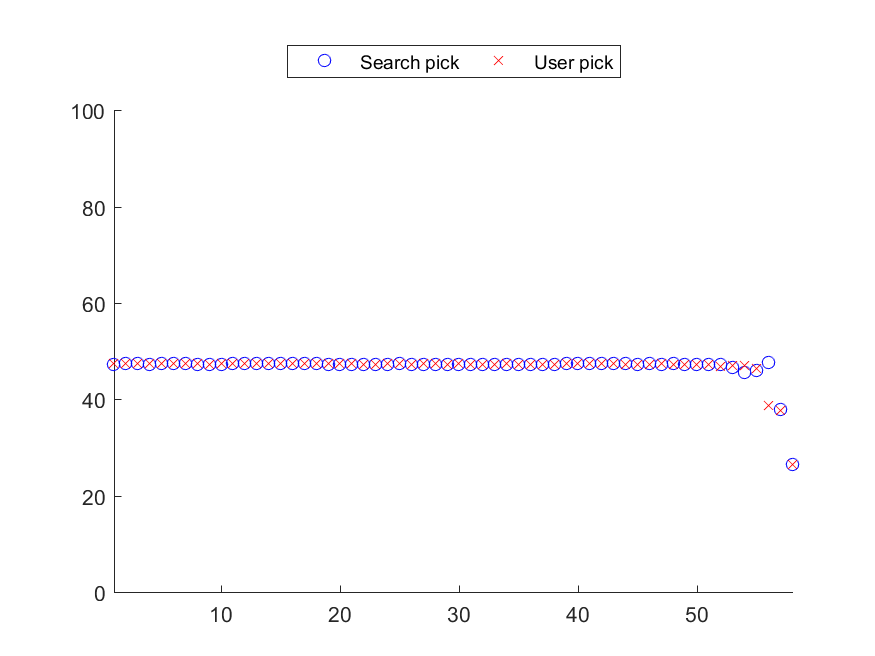
\includegraphics[scale=0.35]{figure/eval/rand/evalMatchskirCh2}}
    \subfloat[][Choleric Match 1 - Random Individual 3] {\includegraphics[scale=0.35]{figure/eval/rand/evalMatchskirCh3}}
    \qquad
    \subfloat[][Melancholic Match 1 - Random Individual 4]{\includegraphics[scale=0.35]{figure/eval/rand/evalMatchskirMe1}}
    \subfloat[][Melancholic Match 1 - Random Individual 5]{\includegraphics[scale=0.35]{figure/eval/rand/evalMatchskirMe4}}
    \subfloat[][Melancholic Match 1 - Random Individual 6]{\includegraphics[scale=0.35]{figure/eval/rand/evalMatchskirMe7}}
    \qquad
    \subfloat[][Sanguine Match 1 - Random Individual 7]{\includegraphics[scale=0.35]{figure/eval/rand/evalMatchskirSa1}}
	\subfloat[][Sanguine Match 1 - Random Individual 8]{\includegraphics[scale=0.35]{figure/eval/rand/evalMatchskirSa4}}
	\subfloat[][Sanguine Match 1 - Random Individual 9]{\includegraphics[scale=0.35]{figure/eval/rand/evalMatchskirSa7}}
	\qquad
    \subfloat[][Phlegmatic Match 1 - Random Individual 10]{\includegraphics[scale=0.35]{figure/eval/rand/evalMatchskirPh1}}
    \subfloat[][Phlegmatic Match 1 - Random Individual 11]{\includegraphics[scale=0.35]{figure/eval/rand/evalMatchskirPh2}}
    \subfloat[][Phlegmatic Match 1 - Random Individual 12]{\includegraphics[scale=0.35]{figure/eval/rand/evalMatchskirPh3}}
    \caption{Evaluation of the Skirmish games with random individuals.}
    \label{fig:randomSkirmish}
\end{figure}
The individuals used have the values shown in table \ref{tab:random}.
\begin{table}[H]
	\caption{Random individuals picked for evaluation.}
    \centering
    \resizebox{\textwidth}{!}{%
    \begin{tabular}{|c|c|c|c|c|c|c|c|c|c|c|c|c|}
    \hline
Parameter & Ind. 1 & Ind. 2 & Ind. 3 & Ind. 4 & Ind. 5 & Ind. 6 & Ind. 7 & Ind. 8 & Ind. 9 & Ind. 10 & Ind. 11 & Ind. 12\\
        \hline
    eps. & 0.299 & 0.540 & 0.205 & 0.206 & 0.617 & 0.191 & 0.757 & 0.778 & 0.292 & 0.308 & 0.155 & 0.394\\
        \hline
    rave & 4508& 1464 & 4904 & 4798 & 285 & 3867 & 3223 & 3778 & 3455 &3818 & 3332 & 4852\\
        \hline
    grave & 88 & 9 & 69 & 117 & 90 & 97 & 67 & 29 & 73 & 15 & 45 & 8\\
        \hline
    chargeDis. &  0.928 & 0.945 & 0.950 & 0.989 & 0.996 & 0.984 & 0.980 & 0.901 & 0.923 & 0.931 & 0.964 & 0.995\\ 
        \hline
    treeDis. & 0.971 & 0.958 & 0.925 & 0.987 & 0.945 & 0.965 & 0.934 & 0.964 & 0.930 & 0.972 & 0.902 & 0.978\\
        \hline
    aggr. & 0.784 & 2.612 & 2.927 & 2.044 & 0.430 & 1.634 & 2.684 & 0.139 & 1.936 & 0.701 & 0.907 & 2.172\\ 
        \hline
    defen. & 1.500 & 1.866 & 1.052 & 1.316 & 0.946 & 0.645 & 1.956 & 1.503 & 0.995 & 1.075 & 0.123 & 2.998\\ 
        \hline
    ch.Depth & 65 & 20 & 94 & 60 & 19 & 67 & 34.248 & 21.756 & 62.990 & 29.706 & 75.676 & 30.799\\ 
        \hline
    horizon & 9 & 7 & 2 & 6 & 17 & 17 & 15 & 19 & 8 & 3 & 3 & 13\\
        \hline
    randErr & 0.290 & 0.485 & 0.248 & 0.754 & 0.075 & 0.392 & 0.427 & 0.624 & 0.450 & 0.095 & 0.566 & 0.024\\
        \hline
    ch.Default & 39.706 & 37.803 & 39.729 & 42.191 & 41.370 & 37.540 & 42.251 & 39.168 & 44.157 & 38.380 & 38.980 & 44.756\\
        \hline
    expl.Fac. & 125 & 81 & 120 & 49 & 36 & 35 & 5 & 13 & 121 & 47 & 137 & 12\\ 
        \hline
    niceTh. & 38.448 & 49.630 & 45.040 & 8.273 & 46.950 & 28.877 & 18.790 & 61.309 &19.282 & 45.644 & 41.199 & 35.793\\
        \hline
    \end{tabular}}
    \label{tab:random}
\end{table}
Approximately, it can be seen the same behaviour as with the "correct" parameter, excused by the magnitude of the state space of the game, as discussed earlier. However, it is possible to see some sloppiness in the search selection, compared to the user's. Figure \ref{fig:skRan} shows the percentage of matching moves having random individuals playing over the matches that were associated to personalities from the data collection. 
\begin{figure}[H]
\centering
	\includegraphics[scale=0.5]{figure/eval/TotRandSk}
    \caption{Actions Agreement Ratio for Skirmish games with random individuals.}
    \label{fig:skRan}
\end{figure}
This result shows an higher average of agreed moves, confirming the hypothesis of the genetic algorithm hitting a local maxima and not returning the optimal individuals, as well as that the personality model adopted might not be correctly modeled.
\subsection{Random Games with Random Individuals}\label{sec:randomrandom}
Lastly, four random individuals (A, B, C, D) have been plugged in the games we have no knowledge about, and the summary of it can be seen in figure \ref{fig:totrandom}. Comparing it with figure \ref{fig:tot}, it can be seen that individual D has more matching moves than the Choleric individual from the genetic algorithm (which was the one with the highest frequency of match, as seen in section \ref{sec:randGamesFitInd}).
\begin{figure}[H]
\centering
	\includegraphics[scale=0.6]{figure/eval/rand/TotRand}
    \caption{Evaluation with Random Individuals (percentage).}
    \label{fig:totrandom}
\end{figure}
The meaning behind this result, in addition to what can be interpreted from the graphs in appendix \ref{sec:genegraphs}, can once more be that the personality model used for this thesis is not a true fit, as well as the genetic algorithm hit a local maxima, and would require some more tweaking to return improved results.
\section{Limitations and Improvements}
The project has been subject to limitations due to both time, and power constraints.\\
The remarkable time complexity of the Genetic Algorithm, together with time constraints, forced us to restrain the number of tests for parameters' tweaking, increasing the chances of hitting a local maxima or having premature stagnancy. More tweaking would lead to better results, overall, but we have to bound this thesis to a few choices of Genetic Algorithm parameters. It is to be recalled also that the geometric mean plotted on the graphs turned out to be slightly different than the one calculated in the genetic algorithm. Further investigations about this matter will have to be performed. In the case this would be fixed, it would be natural to suppose that the average fitness for each generation would be closer to the probability of picking one move at random, at least at initial states.\\
Mostly, however, the limitation lies on the data collection. Due to non-optimal resources, the data this thesis bases itself on, for both training and evaluation, has not been enough to infer a proper state-action distribution and get properly defined results overall. If a larger dataset would be available, it would be interesting to notice how the genetic algorithm would react to a more demanding training, and if the fittest individuals would be a better match for the personality model adopted here. In the case of more training data, it could also be possible to adopt a more detailed personality model, which could help reproducing gameplay more closely. The data to feed the genetic algorithm with will have also to be from more reliable sources, as self-assigning personality might not be accurate. Furthermore, some of our players have been acting other personalities, which could have affected the data in a negative way, considering how hard it could be to suppress emotions in some cases.
Lastly, understanding how the MCTS parameters can be changed, and how they are correlated to each other would supposedly help having more precise individuals as output from the GA.
\section{Evaluation Results}
Recapitulating the results collected during the evaluation process, it can be said that the individuals returned from the genetic algorithm do not have a relevantly better match than random parameters, over games that have been divided on the basis of our personality model. However, applied to a different set of games, random individuals seem to have a better fit (as seen in section \ref{sec:randomrandom}), leading to the idea that a different personality model might be more suitable for gaming styles representation.\\
It is then confirmed from section \ref{sec:skirmishrandom} that equation (\ref{eq:thesis}) is true, however not in a too definite way. It would be ideal if the results would be more polarised.

% CONCLUSION
\chapter{Conclusion}
In order to infer a personality from human played games, a genetic algorithm has been trained with the aid of collected human-played games. The data has been gathered through the Tiltyard server\cite{tiltyard}, which is a platform for General Game Playing where to test and develop General Game Players. General Game Playing is also the framework used in this project (see section \ref{sec:ggp}), where no knowledge of the game is priorly required. This encouraged having a relatively wide selection of games, allowing the users to select any among the games of Checkers, Connect Four, Nine-Boards Tic-Tac-Toe, and Skirmish. The users also provided information about their personality, based on the Galen-Hippocrates' Four Temperaments model (see section \ref{sec:hippocrates}), which has purposely been chosen as model for this thesis due to its simplicity. The games collected have then been partially used to feed a genetic algorithm (see section \ref{sec:gatheory}), where each individual represented a set of parameters for a Monte Carlo Tree Search algorithm (see section \ref{sec:mctstheory}). The Monte Carlo Tree Search is the main algorithm behind the artificial player used in this thesis, and has been supplied with a set of enhancements, each of which is depending on a control variable. The set of those control variables is the aforementioned individual from the genetic algorithm. Once the GA has been running on a set of game representing a specific personality, the fittest individual is selected for evaluation \ref{sec:meteval}. This reduced to 4 different sets of parameters, one for each personality in the model, that have been plugged in the artificial player, and checked with games that have been left out from the training process.\\
The evaluation process consisted in calculating the Action Agreement Ratio (AAR), together with confronting the QValues of the chosen moves as $\Delta_Q$. The results of this evaluation, collected in chapter \ref{sec:results}, proved that many search-selected moves have an imperceptible $\Delta_Q$, whilst still not reaching perfect matching. This could mean that the gaming style achieved is comparable to human's, although not taking the exact same decisions. However, it is still to be confirmed if it is personality biased.\\
The results obtained in this project are promising enough to believe that a probability model could be inferred from games data. Although the dataset collected and utilised as testbed was not adequate to be considered fully statistically relevant, therefore not confirming nor disproving the thesis where a personality model can be inferred from games data, we are confident that a final conclusion can be drawn with further research.\\
Additional focus would be applicable in determining the best MCTS enhancements and how they affect the search; tweaking the GA parameter so to find a better environment for games data training; applying a different personality model that could be better representative of the players' behaviours; and implement some machine learning strategies to capture patterns in actions' selections for different players. However, none of the above would have meaningful results if the dataset would not be remarkably increased.


% REFERENCES / BIBLIOGRAPHY
\cleardoublepage
\bibliographystyle{acm}
\bibliography{include/backmatter/References}


% APPENDICES
\cleardoublepage
\appendix
\renewcommand{\chaptername}{Appendix}
\setcounter{page}{1}
\pagenumbering{Roman}			% Capitalized roman numbering starting from I (one)

\chapter{Preliminaries}\label{app:prel}
In this appendix we have decided to add a survey of the basic notions needed to fully understand the development of this project.
\section{Data Structures}
We will define here the data structures that will be come across during this thesis work. The definitions are adapted from \cite{kleinberg2006algorithm},\cite{russell1995modern} and \cite{west2001introduction}.
\subsection{Graphs}
\begin{definition}
\label{def:graph}
A \textbf{graph} $G$ is a triple consisting of a collection $V$ of \textbf{nodes}, or \textbf{vertex}; a set $E$ of \textbf{edges}, and a relation that associates with each edge two vertices (not necessarily distinct) called its \textbf{endpoints}. In other words, we represent an edge $e\in E$ as a two-element subset of $V:e={u,v}$ for some $u,v\in V$, where $u$ and $v$ are the \textbf{endpoints} of $e$. 
\end{definition}

\subsection{Directed Graphs}
\begin{definition}
\label{def:dirgraph}
A \textbf{directed graph} $G'$ is a graph with a set of nodes $V$, and a set of \textbf{directed edges} $E'$. Each $e'\in E$ is an \textbf{ordered pair (u,v)}. The roles of the nodes are not interchangeable, and we call $u$ the \textbf{tail} of the edge, and $v$ the \textbf{head}. We also say that an edge is an edge \textbf{from} its tail \textbf{to} its head.
\end{definition}

\subsection{Paths and cycles}
\begin{definition}
A \textbf{path} in a graph $G=(V,E)$ is a sequence $H$ of nodes $v_1,v_2,...,v_{k-1}, v_k$ with the property that each consecutive pair $v_i, v_{i+1}$ is joined by an edge in $G$.
\end{definition}
\begin{definition}
A \textbf{cycle} is a path $v_1,v_2,...,v_{k-1}, v_k$ in which $k>2$, the first $k-1$ nodes are all distinct, and $v_k=v_1$. A graph with no cycle is \textbf{acyclic}.
\end{definition}

\subsection{Connected Graphs}
\begin{definition}
A graph $G$ is \textbf{connected} if each pair of vertices in G belongs to a path; otherwise, $G$ is \textbf{disconnected}.
\end{definition}
\begin{definition}
A directed graph is \textbf{strongly connected} if, for every two nodes $u$ and $v$, there is a path from $u$ to $v$ and a path from $v$ to $u$.
\end{definition}

\subsection{Trees}
\begin{definition}
A \textbf{tree} $T$ is a connected acyclic graph. Picked a node $r$ as \textbf{root}, each other edge is oriented away from it. For each node $v$, a \textbf{parent} (or \textbf{ancestor}) of $v$ is defined as the node $u$ that directly precedes $v$ on its path from $r$. A node $w$ is defined \textbf{child} (or \textbf{descendant}) of $v$ if $v$ is the parent of $w$.  A \textbf{leaf} is a vertex with no descendants.
\end{definition}


\subsection{State Space}
\begin{definition}
The \textbf{state space} of a problem is the set of all the states reachable from the initial state by any sequence of actions.
\end{definition}

\section{Finite State-Machines}
State machines are defined as sets of states connected through transitions, which are controlled by inputs. Here we will define them differentiating whether they are deterministic, an example of which can be seen in figure \ref{fig:DFA}, or non-deterministic, as in figure \ref{fig:NFA}. Definitions are adapted from \cite{hopcroft2006automata}; we will be using the terms "state machine" and "automaton" interchangeably.\todo{fix this}

\subsection{Deterministic Finite Automata (DFA)}
\begin{definition}
\label{def:detsm}
A \textbf{deterministic finite automaton} is a tuple $<S, \Sigma, \delta, s_0, \Gamma>$, where:
\begin{itemize}
\item A finite set of \textbf{states} $S$.
\item A finite set of \textbf{input symbols}, or \textbf{alphabet}, $\Sigma$.
\item A \textbf{transition function} that takes as argument a state and an input symbol, and returns a state. The transition function will commonly be denoted $\delta$, and $\delta: S \times \Sigma \rightarrow S$. In informal graph representation of automata, $\delta$ was represented by arcs between states and the labels on the arcs. If $s$ is a state, and $\sigma$ is an input symbol, then $\delta(s,\sigma)$ is the state $q$ such that there is an arc labeled $\sigma$ from $s$ to $q$.
\item A \textbf{start state} $s_0$, one of the states in $S$.
\item A set of \textbf{final} or \textbf{accepting states} $\Gamma$, where $\Gamma \subseteq S$.
\end{itemize}
\end{definition}

\begin{figure}[H]
\centering
\begin{tikzpicture}[->,>=stealth',shorten >=1pt,auto,node distance=2.8cm,
                    semithick]

  \node[initial,state]		(A)              {$s_0$};
  \node[state]				(B) [right of=A] {$s_1$};
  \node[state,accepting]	(C) [right of=B] {$s_2$};

  \path (A) edge              node {1} (B)
        (B) edge [loop above] node {0} (B)
            edge              node {1} (C);
\end{tikzpicture}
\caption{Example of simple DFA.}\label{fig:DFA}
\end{figure}


\subsection{Non-Deterministic Finite Automata (NFA)}
\begin{definition}
\label{def:nondetsm}
A \textbf{non deterministic finite automaton} is a tuple $<S, \Sigma, \delta, s_0, \Gamma>$, where:
\begin{itemize}
\item A finite set of \textbf{states} $S$.
\item A finite set of \textbf{input symbols}, or \textbf{alphabet}, $\Sigma$.
\item A \textbf{transition function} $\delta$ that takes as argument a state and an input symbol, and returns a subset of states, $\delta: S \times \Sigma \rightarrow \mathcal{P}(S)$. 
\item A \textbf{start state} $s_0$, one of the states in $S$.
\item A set of \textbf{final} or \textbf{accepting states} $\Gamma$, where $\Gamma \subseteq S$.
\end{itemize}
\end{definition}

\begin{figure}[H]
\centering
\begin{tikzpicture}[->,>=stealth',shorten >=1pt,auto,node distance=2.8cm,
                    semithick]

  \node[initial,state]		(A)              {$s_0$};
  \node[state]				(B) [right of=A] {$s_1$};
  \node[state,accepting]	(C) [right of=B] {$s_2$};

  \path (A) edge              node {1} (B)
        (B) edge [loop above] node {0,1} (B)
            edge              node {0} (C);
\end{tikzpicture}
\caption{Example of simple NFA.\protect\footnotemark}\label{fig:NFA}
\end{figure}\footnotetext{Note that for state $s_1$ the input $0$ can lead indistinctly to either state $s_1$ or $s_2$.}

\section{Probability}
Here is a small recap on the probability basics needed to understand the logic behind the probability model in section \ref{sec:mlmethod}. This appendix will not contain more formulas and definition than strictly needed, so we refer to \cite{murphy2012machine} for further information.
In this thesis, $P(\mathpzc{E})$ indicates the probability of event $\mathpzc{E}$ being true. It is known that $0\geq P(\mathpzc{E})\geq 1$, where $P(\mathpzc{E})=1$ means the event will certainly happen.
\subsection{Elementary rules}
\begin{definition}[Joint Probability]
Given two events $\mathpzc{A}$ and $\mathpzc{B}$, the probability of both happening jointly is given by the product rule: $$P(\mathpzc{A}\vee\mathpzc{B})=P(\mathpzc{A,B})=P(\mathpzc{A|B})P(\mathpzc{B}).$$
\end{definition}
\begin{definition}[Sum Rule (Marginal Distribution)]
Given a joint distribution of two events $\mathpzc{A,B}$, the marginal distribution is defined as: $$P(\mathpzc{A}=\sum_\mathpzc{b} P(\mathpzc{A,B})=\sum_\mathpzc{b} P(\mathpzc{A|B=b})P(\mathpzc{B=b}).$$
\end{definition}
\begin{definition}[Chain Rule]
Given a set of $\mathpzc{N}$ events $\mathpzc{A_{[1,\ldots,N]}}$ the probability of them happening jointly is given by the chain rule: $$P(\mathpzc{A_{[1,\ldots,N]}}=P(\mathpzc{A_1})P(\mathpzc{A_2|A_1})\ldots P(\mathpzc{A_N|A_{N-1},A_{N-2},\ldots,A_1}).$$
\end{definition}
\begin{definition}[Conditional Probability]
Given two events $\mathpzc{A}$ and $\mathpzc{B}$, the probability of event $\mathpzc{A}$, given that $\mathpzc{B}$ is true, is: $$P(\mathpzc{A|B})=\frac{P(\mathpzc{A,B})}{P(\mathpzc{B})}\qquad\text{if }P(\mathpzc{B}>0).$$
\end{definition}
\begin{definition}[Bayes' Rule]
Given two events $\mathpzc{A}$ and $\mathpzc{B}$, $$P(\mathpzc{A=a|B=b})=\frac{P(\mathpzc{A=a,B=b})}{P(\mathpzc{B=b})}=\frac{P(\mathpzc{A=a})P(\mathpzc{B=b|A=a})}{\sum_a'P(\mathpzc{A=a'})P(\mathpzc{B=b|A=a'})}.$$
\end{definition}

\chapter{Collection of Graphs}\label{sec:genegraphs}
In this appendix chapter it is possible to find a collection of graphs showing the development of the single genes in each individual in the population, throughout the generations. On the y-axis it will be the values accepted for the specific gene, while the x-axis will indicate the generations. The discussion over the following graphs can be found in section \ref{sec:gares}.\\
Hereafter, there are scatter plots of the single genes in each individuals correlated to their fitness value. X-axis represents the interval the gene's values are in, while Y-axis represents a variation of the fitness value. We refer once more to section \ref{sec:gares} for further information.\\
The graphs relative to the evaluation process can be found in this appendix as well, where the x-axis indicates the turns of the game, and the y-axis the Q-value of the actions selected by the search and the users. The graphs will be further discussed in section \ref{sec:reeval}.\\
\newpage
\section{Single Individuals}
\hspace{0pt}
\vfill
\begin{figure}[H]
\centering
    \subfloat[][Choleric - I run] {\includegraphics[scale=0.35]{figure/graphs1run/aggressC}}
    \subfloat[][Choleric - II run] {\includegraphics[scale=0.35]{figure/graphs2run/aggressC}}
	\subfloat[][Choleric - III run] {\includegraphics[scale=0.35]{figure/graphs3run/aggressC}}
    \qquad
    \subfloat[][Melancholic - I run]{\includegraphics[scale=0.35]{figure/graphs1run/aggressM}}
    \subfloat[][Melancholic - II run]{\includegraphics[scale=0.35]{figure/graphs2run/aggressM}}
    \subfloat[][Melancholic - III run]{\includegraphics[scale=0.35]{figure/graphs3run/aggressM}}
    \qquad
    \subfloat[][Sanguine - I run]{\includegraphics[scale=0.35]{figure/graphs1run/aggressS}}
	\subfloat[][Sanguine - II run]{\includegraphics[scale=0.35]{figure/graphs2run/aggressS}}
	\subfloat[][Sanguine - III run]{\includegraphics[scale=0.35]{figure/graphs3run/aggressS}}
	\qquad
    \subfloat[][Phlegmatic - I run]{\includegraphics[scale=0.35]{figure/graphs1run/aggressP}}
    \subfloat[][Phlegmatic - II run]{\includegraphics[scale=0.35]{figure/graphs2run/aggressP}}
    \subfloat[][Phlegmatic - III run]{\includegraphics[scale=0.35]{figure/graphs3run/aggressP}}
  \captionsetup{justification=centering}
    \caption{Aggressiveness gene.}
    \label{fig:aggressiveness}
\end{figure}
\vfill
\hspace{0pt}
\pagebreak
\begin{figure}[H]
\centering
    \subfloat[][Choleric - I run] {\includegraphics[scale=0.35]{figure/graphs1run/chargedefC}}
    \subfloat[][Choleric - II run] {\includegraphics[scale=0.35]{figure/graphs2run/chargedefC}}
	\subfloat[][Choleric - III run] {\includegraphics[scale=0.35]{figure/graphs3run/chargedefC}}
    \qquad
    \subfloat[][Melancholic - I run]{\includegraphics[scale=0.35]{figure/graphs1run/chargedefM}}
    \subfloat[][Melancholic - II run]{\includegraphics[scale=0.35]{figure/graphs2run/chargedefM}}
    \subfloat[][Melancholic - III run]{\includegraphics[scale=0.35]{figure/graphs3run/chargedefM}}
    \qquad
    \subfloat[][Sanguine - I run]{\includegraphics[scale=0.35]{figure/graphs1run/chargedefS}}
	\subfloat[][Sanguine - II run]{\includegraphics[scale=0.35]{figure/graphs2run/chargedefS}}
	\subfloat[][Sanguine - III run]{\includegraphics[scale=0.35]{figure/graphs3run/chargedefS}}
	\qquad
    \subfloat[][Phlegmatic - I run]{\includegraphics[scale=0.35]{figure/graphs1run/chargedefP}}
    \subfloat[][Phlegmatic - II run]{\includegraphics[scale=0.35]{figure/graphs2run/chargedefP}}
    \subfloat[][Phlegmatic - III run]{\includegraphics[scale=0.35]{figure/graphs3run/chargedefP}}
  \captionsetup{justification=centering}
    \caption{Charge Default gene.}
    \label{fig:chargedef}
\end{figure}
\begin{figure}[H]
\centering
    \subfloat[][Choleric - I run] {\includegraphics[scale=0.35]{figure/graphs1run/chargedepthC}}
    \subfloat[][Choleric - II run] {\includegraphics[scale=0.35]{figure/graphs2run/chargedepthC}}
	\subfloat[][Choleric - III run] {\includegraphics[scale=0.35]{figure/graphs3run/chargedepthC}}
    \qquad
    \subfloat[][Melancholic - I run]{\includegraphics[scale=0.35]{figure/graphs1run/chargedepthM}}
    \subfloat[][Melancholic - II run]{\includegraphics[scale=0.35]{figure/graphs2run/chargedepthM}}
    \subfloat[][Melancholic - III run]{\includegraphics[scale=0.35]{figure/graphs3run/chargedepthM}}
    \qquad
    \subfloat[][Sanguine - I run]{\includegraphics[scale=0.35]{figure/graphs1run/chargedepthS}}
	\subfloat[][Sanguine - II run]{\includegraphics[scale=0.35]{figure/graphs2run/chargedepthS}}
	\subfloat[][Sanguine - III run]{\includegraphics[scale=0.35]{figure/graphs3run/chargedepthS}}
	\qquad
    \subfloat[][Phlegmatic - I run]{\includegraphics[scale=0.35]{figure/graphs1run/chargedepthP}}
    \subfloat[][Phlegmatic - II run]{\includegraphics[scale=0.35]{figure/graphs2run/chargedepthP}}
    \subfloat[][Phlegmatic - III run]{\includegraphics[scale=0.35]{figure/graphs3run/chargedepthP}}
  \captionsetup{justification=centering}
    \caption{Charge Depth gene.}
    \label{fig:chargedepth}
\end{figure}
\begin{figure}[H]
\centering
    \subfloat[][Choleric - I run] {\includegraphics[scale=0.35]{figure/graphs1run/chargediscountC}}
    \subfloat[][Choleric - II run] {\includegraphics[scale=0.35]{figure/graphs2run/chargediscountC}}
	\subfloat[][Choleric - III run] {\includegraphics[scale=0.35]{figure/graphs3run/chargediscountC}}
    \qquad
    \subfloat[][Melancholic - I run]{\includegraphics[scale=0.35]{figure/graphs1run/chargediscountM}}
    \subfloat[][Melancholic - II run]{\includegraphics[scale=0.35]{figure/graphs2run/chargediscountM}}
    \subfloat[][Melancholic - III run]{\includegraphics[scale=0.35]{figure/graphs3run/chargediscountM}}
    \qquad
    \subfloat[][Sanguine - I run]{\includegraphics[scale=0.35]{figure/graphs1run/chargediscountS}}
	\subfloat[][Sanguine - II run]{\includegraphics[scale=0.35]{figure/graphs2run/chargediscountS}}
	\subfloat[][Sanguine - III run]{\includegraphics[scale=0.35]{figure/graphs3run/chargediscountS}}
	\qquad
    \subfloat[][Phlegmatic - I run]{\includegraphics[scale=0.35]{figure/graphs1run/chargediscountP}}
    \subfloat[][Phlegmatic - II run]{\includegraphics[scale=0.35]{figure/graphs2run/chargediscountP}}
    \subfloat[][Phlegmatic - III run]{\includegraphics[scale=0.35]{figure/graphs3run/chargediscountP}}
  \captionsetup{justification=centering}
    \caption{Charge Discount gene.}
    \label{fig:chargediscount}
\end{figure}
\begin{figure}[H]
\centering
    \subfloat[][Choleric - I run] {\includegraphics[scale=0.35]{figure/graphs1run/defensivC}}
    \subfloat[][Choleric - II run] {\includegraphics[scale=0.35]{figure/graphs2run/defensivC}}
	\subfloat[][Choleric - III run] {\includegraphics[scale=0.35]{figure/graphs3run/defensivC}}
    \qquad
    \subfloat[][Melancholic - I run]{\includegraphics[scale=0.35]{figure/graphs1run/defensivM}}
    \subfloat[][Melancholic - II run]{\includegraphics[scale=0.35]{figure/graphs2run/defensivM}}
    \subfloat[][Melancholic - III run]{\includegraphics[scale=0.35]{figure/graphs3run/defensivM}}
    \qquad
    \subfloat[][Sanguine - I run]{\includegraphics[scale=0.35]{figure/graphs1run/defensivS}}
	\subfloat[][Sanguine - II run]{\includegraphics[scale=0.35]{figure/graphs2run/defensivS}}
	\subfloat[][Sanguine - III run]{\includegraphics[scale=0.35]{figure/graphs3run/defensivS}}
	\qquad
    \subfloat[][Phlegmatic - I run]{\includegraphics[scale=0.35]{figure/graphs1run/defensivP}}
    \subfloat[][Phlegmatic - II run]{\includegraphics[scale=0.35]{figure/graphs2run/defensivP}}
    \subfloat[][Phlegmatic - III run]{\includegraphics[scale=0.35]{figure/graphs3run/defensivP}}
  \captionsetup{justification=centering}
    \caption{Defensiveness gene.}
    \label{fig:defensiveness}
\end{figure}
\begin{figure}[H]
\centering
    \subfloat[][Choleric - I run] {\includegraphics[scale=0.35]{figure/graphs1run/epsilonC}}
    \subfloat[][Choleric - II run] {\includegraphics[scale=0.35]{figure/graphs2run/epsilonC}}
	\subfloat[][Choleric - III run] {\includegraphics[scale=0.35]{figure/graphs3run/epsilonC}}
    \qquad
    \subfloat[][Melancholic - I run]{\includegraphics[scale=0.35]{figure/graphs1run/epsilonM}}
    \subfloat[][Melancholic - II run]{\includegraphics[scale=0.35]{figure/graphs2run/epsilonM}}
    \subfloat[][Melancholic - III run]{\includegraphics[scale=0.35]{figure/graphs3run/epsilonM}}
    \qquad
    \subfloat[][Sanguine - I run]{\includegraphics[scale=0.35]{figure/graphs1run/epsilonS}}
	\subfloat[][Sanguine - II run]{\includegraphics[scale=0.35]{figure/graphs2run/epsilonS}}
	\subfloat[][Sanguine - III run]{\includegraphics[scale=0.35]{figure/graphs3run/epsilonS}}
	\qquad
    \subfloat[][Phlegmatic - I run]{\includegraphics[scale=0.35]{figure/graphs1run/epsilonP}}
    \subfloat[][Phlegmatic - II run]{\includegraphics[scale=0.35]{figure/graphs2run/epsilonP}}
    \subfloat[][Phlegmatic - III run]{\includegraphics[scale=0.35]{figure/graphs3run/epsilonP}}
  \captionsetup{justification=centering}
    \caption{Epsilon gene.}
    \label{fig:epsilon}
\end{figure}
\begin{figure}[H]
\centering
    \subfloat[][Choleric - I run] {\includegraphics[scale=0.35]{figure/graphs1run/explfactC}}
    \subfloat[][Choleric - II run] {\includegraphics[scale=0.35]{figure/graphs2run/explfactC}}
	\subfloat[][Choleric - III run] {\includegraphics[scale=0.35]{figure/graphs3run/explfactC}}
    \qquad
    \subfloat[][Melancholic - I run]{\includegraphics[scale=0.35]{figure/graphs1run/explfactM}}
    \subfloat[][Melancholic - II run]{\includegraphics[scale=0.35]{figure/graphs2run/explfactM}}
    \subfloat[][Melancholic - III run]{\includegraphics[scale=0.35]{figure/graphs3run/explfactM}}
    \qquad
    \subfloat[][Sanguine - I run]{\includegraphics[scale=0.35]{figure/graphs1run/explfactS}}
	\subfloat[][Sanguine - II run]{\includegraphics[scale=0.35]{figure/graphs2run/explfactS}}
	\subfloat[][Sanguine - III run]{\includegraphics[scale=0.35]{figure/graphs3run/explfactS}}
	\qquad
    \subfloat[][Phlegmatic - I run]{\includegraphics[scale=0.35]{figure/graphs1run/explfactP}}
    \subfloat[][Phlegmatic - II run]{\includegraphics[scale=0.35]{figure/graphs2run/explfactP}}
    \subfloat[][Phlegmatic - III run]{\includegraphics[scale=0.35]{figure/graphs3run/explfactP}}
  \captionsetup{justification=centering}
    \caption{Exploration Factor gene.}
    \label{fig:explfact}
\end{figure}
\begin{figure}[H]
\centering
    \subfloat[][Choleric - I run] {\includegraphics[scale=0.35]{figure/graphs1run/graveC}}
    \subfloat[][Choleric - II run] {\includegraphics[scale=0.35]{figure/graphs2run/graveC}}
	\subfloat[][Choleric - III run] {\includegraphics[scale=0.35]{figure/graphs3run/graveC}}
    \qquad
    \subfloat[][Melancholic - I run]{\includegraphics[scale=0.35]{figure/graphs1run/graveM}}
    \subfloat[][Melancholic - II run]{\includegraphics[scale=0.35]{figure/graphs2run/graveM}}
    \subfloat[][Melancholic - III run]{\includegraphics[scale=0.35]{figure/graphs3run/graveM}}
    \qquad
    \subfloat[][Sanguine - I run]{\includegraphics[scale=0.35]{figure/graphs1run/graveS}}
	\subfloat[][Sanguine - II run]{\includegraphics[scale=0.35]{figure/graphs2run/graveS}}
	\subfloat[][Sanguine - III run]{\includegraphics[scale=0.35]{figure/graphs3run/graveS}}
	\qquad
    \subfloat[][Phlegmatic - I run]{\includegraphics[scale=0.35]{figure/graphs1run/graveP}}
    \subfloat[][Phlegmatic - II run]{\includegraphics[scale=0.35]{figure/graphs2run/graveP}}
    \subfloat[][Phlegmatic - III run]{\includegraphics[scale=0.35]{figure/graphs3run/graveP}}
  \captionsetup{justification=centering}
    \caption{Grave gene.}
    \label{fig:grave}
\end{figure}
\begin{figure}[H]
\centering
    \subfloat[][Choleric - I run] {\includegraphics[scale=0.35]{figure/graphs1run/horizonC}}
    \subfloat[][Choleric - II run] {\includegraphics[scale=0.35]{figure/graphs2run/horizonC}}
	\subfloat[][Choleric - III run] {\includegraphics[scale=0.35]{figure/graphs3run/horizonC}}
    \qquad
    \subfloat[][Melancholic - I run]{\includegraphics[scale=0.35]{figure/graphs1run/horizonM}}
    \subfloat[][Melancholic - II run]{\includegraphics[scale=0.35]{figure/graphs2run/horizonM}}
    \subfloat[][Melancholic - III run]{\includegraphics[scale=0.35]{figure/graphs3run/horizonM}}
    \qquad
    \subfloat[][Sanguine - I run]{\includegraphics[scale=0.35]{figure/graphs1run/horizonS}}
	\subfloat[][Sanguine - II run]{\includegraphics[scale=0.35]{figure/graphs2run/horizonS}}
	\subfloat[][Sanguine - III run]{\includegraphics[scale=0.35]{figure/graphs3run/horizonS}}
	\qquad
    \subfloat[][Phlegmatic - I run]{\includegraphics[scale=0.35]{figure/graphs1run/horizonP}}
    \subfloat[][Phlegmatic - II run]{\includegraphics[scale=0.35]{figure/graphs2run/horizonP}}
    \subfloat[][Phlegmatic - III run]{\includegraphics[scale=0.35]{figure/graphs3run/horizonP}}
  \captionsetup{justification=centering}
    \caption{Horizon gene.}
    \label{fig:horizon}
\end{figure}
\begin{figure}[H]
\centering
    \subfloat[][Choleric - I run] {\includegraphics[scale=0.35]{figure/graphs1run/nicethresC}}
    \subfloat[][Choleric - II run] {\includegraphics[scale=0.35]{figure/graphs2run/nicethresC}}
	\subfloat[][Choleric - III run] {\includegraphics[scale=0.35]{figure/graphs3run/nicethresC}}
    \qquad
    \subfloat[][Melancholic - I run]{\includegraphics[scale=0.35]{figure/graphs1run/nicethresM}}
    \subfloat[][Melancholic - II run]{\includegraphics[scale=0.35]{figure/graphs2run/nicethresM}}
    \subfloat[][Melancholic - III run]{\includegraphics[scale=0.35]{figure/graphs3run/nicethresM}}
    \qquad
    \subfloat[][Sanguine - I run]{\includegraphics[scale=0.35]{figure/graphs1run/nicethresS}}
	\subfloat[][Sanguine - II run]{\includegraphics[scale=0.35]{figure/graphs2run/nicethresS}}
	\subfloat[][Sanguine - III run]{\includegraphics[scale=0.35]{figure/graphs3run/nicethresS}}
	\qquad
    \subfloat[][Phlegmatic - I run]{\includegraphics[scale=0.35]{figure/graphs1run/nicethresP}}
    \subfloat[][Phlegmatic - II run]{\includegraphics[scale=0.35]{figure/graphs2run/nicethresP}}
    \subfloat[][Phlegmatic - III run]{\includegraphics[scale=0.35]{figure/graphs3run/nicethresP}}
  \captionsetup{justification=centering}
    \caption{Nice Threshold gene.}
    \label{fig:nicethres}
\end{figure}
\begin{figure}[H]
\centering
    \subfloat[][Choleric - I run] {\includegraphics[scale=0.35]{figure/graphs1run/randomerrorC}}
    \subfloat[][Choleric - II run] {\includegraphics[scale=0.35]{figure/graphs2run/randomerrorC}}
	\subfloat[][Choleric - III run] {\includegraphics[scale=0.35]{figure/graphs3run/randomerrorC}}
    \qquad
    \subfloat[][Melancholic - I run]{\includegraphics[scale=0.35]{figure/graphs1run/randomerrorM}}
    \subfloat[][Melancholic - II run]{\includegraphics[scale=0.35]{figure/graphs2run/randomerrorM}}
    \subfloat[][Melancholic - III run]{\includegraphics[scale=0.35]{figure/graphs3run/randomerrorM}}
    \qquad
    \subfloat[][Sanguine - I run]{\includegraphics[scale=0.35]{figure/graphs1run/randomerrorS}}
	\subfloat[][Sanguine - II run]{\includegraphics[scale=0.35]{figure/graphs2run/randomerrorS}}
	\subfloat[][Sanguine - III run]{\includegraphics[scale=0.35]{figure/graphs3run/randomerrorS}}
	\qquad
    \subfloat[][Phlegmatic - I run]{\includegraphics[scale=0.35]{figure/graphs1run/randomerrorP}}
    \subfloat[][Phlegmatic - II run]{\includegraphics[scale=0.35]{figure/graphs2run/randomerrorP}}
    \subfloat[][Phlegmatic - III run]{\includegraphics[scale=0.35]{figure/graphs3run/randomerrorP}}
  \captionsetup{justification=centering}
    \caption{Random Error gene.}
    \label{fig:randomerror}
\end{figure}
\begin{figure}[H]
\centering
    \subfloat[][Choleric - I run] {\includegraphics[scale=0.35]{figure/graphs1run/raveC}}
    \subfloat[][Choleric - II run] {\includegraphics[scale=0.35]{figure/graphs2run/raveC}}
	\subfloat[][Choleric - III run] {\includegraphics[scale=0.35]{figure/graphs3run/raveC}}
    \qquad
    \subfloat[][Melancholic - I run]{\includegraphics[scale=0.35]{figure/graphs1run/raveM}}
    \subfloat[][Melancholic - II run]{\includegraphics[scale=0.35]{figure/graphs2run/raveM}}
    \subfloat[][Melancholic - III run]{\includegraphics[scale=0.35]{figure/graphs3run/raveM}}
    \qquad
    \subfloat[][Sanguine - I run]{\includegraphics[scale=0.35]{figure/graphs1run/raveS}}
	\subfloat[][Sanguine - II run]{\includegraphics[scale=0.35]{figure/graphs2run/raveS}}
	\subfloat[][Sanguine - III run]{\includegraphics[scale=0.35]{figure/graphs3run/raveS}}
	\qquad
    \subfloat[][Phlegmatic - I run]{\includegraphics[scale=0.35]{figure/graphs1run/raveP}}
    \subfloat[][Phlegmatic - II run]{\includegraphics[scale=0.35]{figure/graphs2run/raveP}}
    \subfloat[][Phlegmatic - III run]{\includegraphics[scale=0.35]{figure/graphs3run/raveP}}
  \captionsetup{justification=centering}
    \caption{Rave gene.}
    \label{fig:rave}
\end{figure}
\begin{figure}[H]
\centering
    \subfloat[][Choleric - I run] {\includegraphics[scale=0.35]{figure/graphs1run/treediscountC}}
    \subfloat[][Choleric - II run] {\includegraphics[scale=0.35]{figure/graphs2run/treediscountC}}
	\subfloat[][Choleric - III run] {\includegraphics[scale=0.35]{figure/graphs3run/treediscountC}}
    \qquad
    \subfloat[][Melancholic - I run]{\includegraphics[scale=0.35]{figure/graphs1run/treediscountM}}
    \subfloat[][Melancholic - II run]{\includegraphics[scale=0.35]{figure/graphs2run/treediscountM}}
    \subfloat[][Melancholic - III run]{\includegraphics[scale=0.35]{figure/graphs3run/treediscountM}}
    \qquad
    \subfloat[][Sanguine - I run]{\includegraphics[scale=0.35]{figure/graphs1run/treediscountS}}
	\subfloat[][Sanguine - II run]{\includegraphics[scale=0.35]{figure/graphs2run/treediscountS}}
	\subfloat[][Sanguine - III run]{\includegraphics[scale=0.35]{figure/graphs3run/treediscountS}}
	\qquad
    \subfloat[][Phlegmatic - I run]{\includegraphics[scale=0.35]{figure/graphs1run/treediscountP}}
    \subfloat[][Phlegmatic - II run]{\includegraphics[scale=0.35]{figure/graphs2run/treediscountP}}
    \subfloat[][Phlegmatic - III run]{\includegraphics[scale=0.35]{figure/graphs3run/treediscountP}}
  \captionsetup{justification=centering}
    \caption{Tree Discount gene.}
    \label{fig:treediscount}
\end{figure}
\begin{figure}[H]
\centering
    \subfloat[][Aggressiveness] {\includegraphics[scale=0.4]{figure/indfit/aggressfit}}
    \subfloat[][Charge Default] {\includegraphics[scale=0.4]{figure/indfit/chargedeffit}}
    \qquad
	\subfloat[][Charge Depth] {\includegraphics[scale=0.4]{figure/indfit/chargedepthfit}}
    \subfloat[][Charge Discount] {\includegraphics[scale=0.4]{figure/indfit/chargediscountfit}}
    \qquad
    \subfloat[][Defensiveness]{\includegraphics[scale=0.4]{figure/indfit/defensivfit}}
    \subfloat[][Epsilon]{\includegraphics[scale=0.4]{figure/indfit/epsilonfit}}
    \qquad
    \subfloat[][Exploration Factor]{\includegraphics[scale=0.4]{figure/indfit/explfactfit}}
  \captionsetup{justification=centering}
    \caption{Correlation between specific genes and fitness (continued on the next page).}
    \label{fig:genescorr}
\end{figure}
\begin{figure}[H]
\centering
	\subfloat[][Grave]		{\includegraphics[scale=0.4]{figure/indfit/gravefit}}
    \subfloat[][Horizon] {\includegraphics[scale=0.4]{figure/indfit/horizonfit}}
    \qquad
    \subfloat[][Nice Threshold] {\includegraphics[scale=0.4]{figure/indfit/nicethresfit}}
	\subfloat[][Random Error] {\includegraphics[scale=0.4]{figure/indfit/randomerrorfit}}
    \qquad
    \subfloat[][Rave]{\includegraphics[scale=0.4]{figure/indfit/ravefit}}
    \subfloat[][Tree Discount]{\includegraphics[scale=0.4]{figure/indfit/treediscountfit}}
  \captionsetup{justification=centering}
    \caption{Correlation between specific genes and fitness.}
    \label{fig:genescorr2}
\end{figure}
%%%%%%%%%%%%%%%%%%%%%%%%%%%%%%%%%
\section{Evaluation}\label{app:eval}
\begin{figure}[H]
\centering
    \subfloat[][Choleric - Skirmish - Match 1] {\includegraphics[scale=0.35]{figure/eval/Skirmish/evalMatchskirCh1}}
    \qquad
    \subfloat[][Melancholic - Skirmish  - Match 1]{\includegraphics[scale=0.35]{figure/eval/Skirmish/evalMatchskirMe1}}
    \subfloat[][Melancholic - Skirmish  - Match 2]{\includegraphics[scale=0.35]{figure/eval/Skirmish/evalMatchskirMe2}}
    \subfloat[][Melancholic - Skirmish  - Match 3]{\includegraphics[scale=0.35]{figure/eval/Skirmish/evalMatchskirMe3}}
    \qquad
    \subfloat[][Sanguine - Skirmish  - Match 1]{\includegraphics[scale=0.35]{figure/eval/Skirmish/evalMatchskirSa1}}
	\subfloat[][Sanguine - Skirmish  - Match 2]{\includegraphics[scale=0.35]{figure/eval/Skirmish/evalMatchskirSa2}}
	\subfloat[][Sanguine - Skirmish  - Match 3]{\includegraphics[scale=0.35]{figure/eval/Skirmish/evalMatchskirSa3}}
	\qquad
    \subfloat[][Phlegmatic - Skirmish  - Match 1]{\includegraphics[scale=0.35]{figure/eval/Skirmish/evalMatchskirPh1}}
    \caption{Evaluation of the Skirmish games with fittest individuals.}
    \label{fig:evalSkirmish}
\end{figure}
\begin{figure}[H]
\centering
    \subfloat[][Match n.2] {\includegraphics[scale=0.35]{figure/eval/TTTSa/evalMatchnbttt2}}
    \subfloat[][Match n.4] {\includegraphics[scale=0.35]{figure/eval/TTTSa/evalMatchnbttt4}}
	\subfloat[][Match n.8] {\includegraphics[scale=0.35]{figure/eval/TTTSa/evalMatchnbttt8}}
    \qquad
    \subfloat[][Match n.9]{\includegraphics[scale=0.35]{figure/eval/TTTSa/evalMatchnbttt9}}
    \subfloat[][Match n.10]{\includegraphics[scale=0.35]{figure/eval/TTTSa/evalMatchnbttt10}}
    \subfloat[][Match n.12]{\includegraphics[scale=0.35]{figure/eval/TTTSa/evalMatchnbttt12}}
    \qquad
    \subfloat[][Match n.18]{\includegraphics[scale=0.35]{figure/eval/TTTSa/evalMatchnbttt18}}
	\subfloat[][Match n.19]{\includegraphics[scale=0.35]{figure/eval/TTTSa/evalMatchnbttt19}}
	\subfloat[][Match n.20]{\includegraphics[scale=0.35]{figure/eval/TTTSa/evalMatchnbttt20}}
	\qquad
    \subfloat[][Match n.21]{\includegraphics[scale=0.35]{figure/eval/TTTSa/evalMatchnbttt21}}
    \subfloat[][Match n.23]{\includegraphics[scale=0.35]{figure/eval/TTTSa/evalMatchnbttt23}}
    \subfloat[][Match n.24]{\includegraphics[scale=0.35]{figure/eval/TTTSa/evalMatchnbttt24}}
  \captionsetup{justification=centering}
    \caption{Evaluation of Nine Boards Tic-Tac-Toe for Sanguine Personality.}
    \label{fig:nbtttsa}
\end{figure}
\begin{figure}[H]
\centering
    \subfloat[][Match n.2] {\includegraphics[scale=0.35]{figure/eval/TTTPh/evalMatchnbttt2}}
    \subfloat[][Match n.3] {\includegraphics[scale=0.35]{figure/eval/TTTPh/evalMatchnbttt3}}
	\subfloat[][Match n.4] {\includegraphics[scale=0.35]{figure/eval/TTTPh/evalMatchnbttt4}}
    \qquad
    \subfloat[][Match n.5]{\includegraphics[scale=0.35]{figure/eval/TTTPh/evalMatchnbttt5}}
    \subfloat[][Match n.8]{\includegraphics[scale=0.35]{figure/eval/TTTPh/evalMatchnbttt8}}
    \subfloat[][Match n.10]{\includegraphics[scale=0.35]{figure/eval/TTTPh/evalMatchnbttt10}}
    \qquad
    \subfloat[][Match n.13]{\includegraphics[scale=0.35]{figure/eval/TTTPh/evalMatchnbttt13}}
	\subfloat[][Match n.16]{\includegraphics[scale=0.35]{figure/eval/TTTPh/evalMatchnbttt16}}
	\subfloat[][Match n.18]{\includegraphics[scale=0.35]{figure/eval/TTTPh/evalMatchnbttt18}}
	\qquad
    \subfloat[][Match n.20]{\includegraphics[scale=0.35]{figure/eval/TTTPh/evalMatchnbttt20}}
    \subfloat[][Match n.21]{\includegraphics[scale=0.35]{figure/eval/TTTPh/evalMatchnbttt21}}
    \subfloat[][Match n.23]{\includegraphics[scale=0.35]{figure/eval/TTTPh/evalMatchnbttt23}}
  \captionsetup{justification=centering}
    \caption{Evaluation of Nine Boards Tic-Tac-Toe for Phlegmatic Personality.}
    \label{fig:nbtttph}
\end{figure}
\begin{figure}[H]
\centering
    \subfloat[][Match n.2] {\includegraphics[scale=0.35]{figure/eval/TTTMe/evalMatchnbttt2}}
    \subfloat[][Match n.3] {\includegraphics[scale=0.35]{figure/eval/TTTMe/evalMatchnbttt3}}
	\subfloat[][Match n.4] {\includegraphics[scale=0.35]{figure/eval/TTTMe/evalMatchnbttt4}}
    \qquad
    \subfloat[][Match n.5]{\includegraphics[scale=0.35]{figure/eval/TTTMe/evalMatchnbttt5}}
    \subfloat[][Match n.8]{\includegraphics[scale=0.35]{figure/eval/TTTMe/evalMatchnbttt8}}
    \subfloat[][Match n.9]{\includegraphics[scale=0.35]{figure/eval/TTTMe/evalMatchnbttt9}}
    \qquad
    \subfloat[][Match n.10]{\includegraphics[scale=0.35]{figure/eval/TTTMe/evalMatchnbttt10}}
	\subfloat[][Match n.15]{\includegraphics[scale=0.35]{figure/eval/TTTMe/evalMatchnbttt15}}
	\subfloat[][Match n.16]{\includegraphics[scale=0.35]{figure/eval/TTTMe/evalMatchnbttt16}}
	\qquad
    \subfloat[][Match n.19]{\includegraphics[scale=0.35]{figure/eval/TTTMe/evalMatchnbttt19}}
    \subfloat[][Match n.22]{\includegraphics[scale=0.35]{figure/eval/TTTMe/evalMatchnbttt22}}
    \subfloat[][Match n.23]{\includegraphics[scale=0.35]{figure/eval/TTTMe/evalMatchnbttt23}}
  \captionsetup{justification=centering}
    \caption{Evaluation of Nine Boards Tic-Tac-Toe for Melancholic Personality.}
    \label{fig:nbtttme}
\end{figure}
\begin{figure}[H]
\centering
    \subfloat[][Match n.3] {\includegraphics[scale=0.35]{figure/eval/TTTCh/evalMatchnbttt3}}
    \subfloat[][Match n.4] {\includegraphics[scale=0.35]{figure/eval/TTTCh/evalMatchnbttt4}}
	\subfloat[][Match n.6] {\includegraphics[scale=0.35]{figure/eval/TTTCh/evalMatchnbttt6}}
    \qquad
    \subfloat[][Match n.5]{\includegraphics[scale=0.35]{figure/eval/TTTCh/evalMatchnbttt5}}
    \subfloat[][Match n.8]{\includegraphics[scale=0.35]{figure/eval/TTTCh/evalMatchnbttt8}}
    \subfloat[][Match n.10]{\includegraphics[scale=0.35]{figure/eval/TTTCh/evalMatchnbttt10}}
    \qquad
    \subfloat[][Match n.13]{\includegraphics[scale=0.35]{figure/eval/TTTCh/evalMatchnbttt13}}
	\subfloat[][Match n.16]{\includegraphics[scale=0.35]{figure/eval/TTTCh/evalMatchnbttt16}}
	\subfloat[][Match n.18]{\includegraphics[scale=0.35]{figure/eval/TTTCh/evalMatchnbttt18}}
	\qquad
    \subfloat[][Match n.20]{\includegraphics[scale=0.35]{figure/eval/TTTCh/evalMatchnbttt20}}
    \subfloat[][Match n.23]{\includegraphics[scale=0.35]{figure/eval/TTTCh/evalMatchnbttt23}}
    \subfloat[][Match n.24]{\includegraphics[scale=0.35]{figure/eval/TTTCh/evalMatchnbttt24}}
  \captionsetup{justification=centering}
    \caption{Evaluation of Nine Boards Tic-Tac-Toe for Choleric Personality.}
    \label{fig:nbtttch}
\end{figure}
\begin{figure}[H]
\centering
    \subfloat[][Match n.2] {\includegraphics[scale=0.35]{figure/eval/C4Sa/evalMatchc42}}
    \subfloat[][Match n.5] {\includegraphics[scale=0.35]{figure/eval/C4Sa/evalMatchc45}}
	\subfloat[][Match n.9] {\includegraphics[scale=0.35]{figure/eval/C4Sa/evalMatchc49}}
    \qquad
    \subfloat[][Match n.11]{\includegraphics[scale=0.35]{figure/eval/C4Sa/evalMatchc411}}
    \subfloat[][Match n.12]{\includegraphics[scale=0.35]{figure/eval/C4Sa/evalMatchc412}}
    \subfloat[][Match n.13]{\includegraphics[scale=0.35]{figure/eval/C4Sa/evalMatchc413}}
    \qquad
    \subfloat[][Match n.14]{\includegraphics[scale=0.35]{figure/eval/C4Sa/evalMatchc414}}
	\subfloat[][Match n.16]{\includegraphics[scale=0.35]{figure/eval/C4Sa/evalMatchc416}}
	\subfloat[][Match n.18]{\includegraphics[scale=0.35]{figure/eval/C4Sa/evalMatchc418}}
	\qquad
    \subfloat[][Match n.19]{\includegraphics[scale=0.35]{figure/eval/C4Sa/evalMatchc419}}
    \subfloat[][Match n.20]{\includegraphics[scale=0.35]{figure/eval/C4Sa/evalMatchc420}}
    \subfloat[][Match n.22]{\includegraphics[scale=0.35]{figure/eval/C4Sa/evalMatchc422}}
  \captionsetup{justification=centering}
    \caption{Evaluation of Connect Four for Sanguine Personality.}
    \label{fig:c4sa}
\end{figure}
\begin{figure}[H]
\centering
    \subfloat[][Match n.2] {\includegraphics[scale=0.35]{figure/eval/C4Ph/evalMatchc42}}
    \subfloat[][Match n.4] {\includegraphics[scale=0.35]{figure/eval/C4Ph/evalMatchc44}}
	\subfloat[][Match n.5] {\includegraphics[scale=0.35]{figure/eval/C4Ph/evalMatchc45}}
    \qquad
    \subfloat[][Match n.8]{\includegraphics[scale=0.35]{figure/eval/C4Ph/evalMatchc48}}
    \subfloat[][Match n.9]{\includegraphics[scale=0.35]{figure/eval/C4Ph/evalMatchc49}}
    \subfloat[][Match n.11]{\includegraphics[scale=0.35]{figure/eval/C4Ph/evalMatchc411}}
    \qquad    
	\subfloat[][Match n.12]{\includegraphics[scale=0.35]{figure/eval/C4Ph/evalMatchc412}}
	\subfloat[][Match n.14]{\includegraphics[scale=0.35]{figure/eval/C4Ph/evalMatchc414}}
    \subfloat[][Match n.18]{\includegraphics[scale=0.35]{figure/eval/C4Ph/evalMatchc418}}
    \qquad
    \subfloat[][Match n.19]{\includegraphics[scale=0.35]{figure/eval/C4Ph/evalMatchc419}}
    \subfloat[][Match n.20]{\includegraphics[scale=0.35]{figure/eval/C4Ph/evalMatchc420}}
    \subfloat[][Match n.21]{\includegraphics[scale=0.35]{figure/eval/C4Ph/evalMatchc421}}
  \captionsetup{justification=centering}
    \caption{Evaluation of Connect Four for Phlegmatic Personality.}
    \label{fig:c4ph}
\end{figure}
\begin{figure}[H]
\centering
    \subfloat[][Match n.2] {\includegraphics[scale=0.35]{figure/eval/C4Mel/evalMatchc42}}
    \subfloat[][Match n.5] {\includegraphics[scale=0.35]{figure/eval/C4Mel/evalMatchc45}}
	\subfloat[][Match n.7] {\includegraphics[scale=0.35]{figure/eval/C4Mel/evalMatchc47}}
    \qquad
    \subfloat[][Match n.10]{\includegraphics[scale=0.35]{figure/eval/C4Mel/evalMatchc410}}
    \subfloat[][Match n.12]{\includegraphics[scale=0.35]{figure/eval/C4Mel/evalMatchc412}}
    \subfloat[][Match n.13]{\includegraphics[scale=0.35]{figure/eval/C4Mel/evalMatchc413}}
    \qquad
    \subfloat[][Match n.14]{\includegraphics[scale=0.35]{figure/eval/C4Mel/evalMatchc414}}
	\subfloat[][Match n.18]{\includegraphics[scale=0.35]{figure/eval/C4Mel/evalMatchc418}}
	\subfloat[][Match n.19]{\includegraphics[scale=0.35]{figure/eval/C4Mel/evalMatchc419}}
	\qquad
    \subfloat[][Match n.20]{\includegraphics[scale=0.35]{figure/eval/C4Mel/evalMatchc420}}
    \subfloat[][Match n.21]{\includegraphics[scale=0.35]{figure/eval/C4Mel/evalMatchc421}}
    \subfloat[][Match n.22]{\includegraphics[scale=0.35]{figure/eval/C4Mel/evalMatchc422}}
  \captionsetup{justification=centering}
    \caption{Evaluation of Connect Four for Melancholic Personality.}
    \label{fig:c4me}
\end{figure}
\begin{figure}[H]
\centering
    \subfloat[][Match n.2] {\includegraphics[scale=0.35]{figure/eval/C4Ch/evalMatchc42}}
    \subfloat[][Match n.3] {\includegraphics[scale=0.35]{figure/eval/C4Ch/evalMatchc43}}
	\subfloat[][Match n.5] {\includegraphics[scale=0.35]{figure/eval/C4Ch/evalMatchc45}}
    \qquad
    \subfloat[][Match n.10]{\includegraphics[scale=0.35]{figure/eval/C4Ch/evalMatchc410}}
    \subfloat[][Match n.12]{\includegraphics[scale=0.35]{figure/eval/C4Ch/evalMatchc412}}
    \subfloat[][Match n.13]{\includegraphics[scale=0.35]{figure/eval/C4Ch/evalMatchc413}}
    \qquad
    \subfloat[][Match n.16]{\includegraphics[scale=0.35]{figure/eval/C4Ch/evalMatchc416}}
    \subfloat[][Match n.18]{\includegraphics[scale=0.35]{figure/eval/C4Ch/evalMatchc418}}
	\subfloat[][Match n.19]{\includegraphics[scale=0.35]{figure/eval/C4Ch/evalMatchc419}}
    \qquad
	\subfloat[][Match n.20]{\includegraphics[scale=0.35]{figure/eval/C4Ch/evalMatchc420}}
    \subfloat[][Match n.21]{\includegraphics[scale=0.35]{figure/eval/C4Ch/evalMatchc421}}
    \subfloat[][Match n.22]{\includegraphics[scale=0.35]{figure/eval/C4Ch/evalMatchc422}}
  \captionsetup{justification=centering}
    \caption{Evaluation of Connect Four for Choleric Personality.}
    \label{fig:c4ch}
\end{figure}
\begin{figure}[H]
\centering
    \subfloat[][Sanguine - Match 1] {\includegraphics[scale=0.35]{figure/eval/ChSa/evalMatchcheck2}}
    \subfloat[][Sanguine - Match 2] {\includegraphics[scale=0.35]{figure/eval/ChSa/evalMatchcheck4}}
	\subfloat[][Sanguine - Match 3] {\includegraphics[scale=0.35]{figure/eval/ChSa/evalMatchcheck6}}
    \qquad
    \subfloat[][Phlegmatic - Match 1]{\includegraphics[scale=0.35]{figure/eval/ChPh/evalMatchcheck1}}
    \subfloat[][Phlegmatic - Match 2]{\includegraphics[scale=0.35]{figure/eval/ChPh/evalMatchcheck2}}
    \subfloat[][Phlegmatic - Match 4]{\includegraphics[scale=0.35]{figure/eval/ChPh/evalMatchcheck4}}
    \qquad
    \subfloat[][Melancholic - Match 1]{\includegraphics[scale=0.35]{figure/eval/ChMel/evalMatchcheck1}}
	\subfloat[][Melancholic - Match 4]{\includegraphics[scale=0.35]{figure/eval/ChMel/evalMatchcheck4}}
	\subfloat[][Melancholic - Match 6]{\includegraphics[scale=0.35]{figure/eval/ChMel/evalMatchcheck6}}
	\qquad
    \subfloat[][Choleric - Match 2]{\includegraphics[scale=0.35]{figure/eval/ChCh/evalMatchcheck2}}
    \subfloat[][Choleric - Match 4]{\includegraphics[scale=0.35]{figure/eval/ChCh/evalMatchcheck4}}
    \subfloat[][Choleric - Match 6]{\includegraphics[scale=0.35]{figure/eval/ChCh/evalMatchcheck6}}
  \captionsetup{justification=centering}
    \caption{Evaluation of Checkers Games.}
    \label{fig:checkerseval}
\end{figure}
\begin{figure}[H]
\centering
    \subfloat[][Match n.2] {\includegraphics[scale=0.35]{figure/eval/rand/evalMatchnbtttUn2}}
    \subfloat[][Match n.4] {\includegraphics[scale=0.35]{figure/eval/rand/evalMatchnbtttUn4}}
	\subfloat[][Match n.8] {\includegraphics[scale=0.35]{figure/eval/rand/evalMatchnbtttUn8}}
    \qquad
    \subfloat[][Match n.9]{\includegraphics[scale=0.35]{figure/eval/rand/evalMatchnbtttUn9}}
    \subfloat[][Match n.10]{\includegraphics[scale=0.35]{figure/eval/rand/evalMatchnbtttUn10}}
    \subfloat[][Match n.12]{\includegraphics[scale=0.35]{figure/eval/rand/evalMatchnbtttUn12}}
    \qquad
    \subfloat[][Match n.18]{\includegraphics[scale=0.35]{figure/eval/rand/evalMatchnbtttUn18}}
	\subfloat[][Match n.19]{\includegraphics[scale=0.35]{figure/eval/rand/evalMatchnbtttUn19}}
	\subfloat[][Match n.20]{\includegraphics[scale=0.35]{figure/eval/rand/evalMatchnbtttUn20}}
	\qquad
    \subfloat[][Match n.21]{\includegraphics[scale=0.35]{figure/eval/rand/evalMatchnbtttUn21}}
    \subfloat[][Match n.23]{\includegraphics[scale=0.35]{figure/eval/rand/evalMatchnbtttUn23}}
    \subfloat[][Match n.24]{\includegraphics[scale=0.35]{figure/eval/rand/evalMatchnbtttUn24}}
  \captionsetup{justification=centering}
    \caption{Evaluation of Nine Boards Tic-Tac-Toe for Random Individual A.}
    \label{fig:nbranda}
\end{figure}
\begin{figure}[H]
\centering
    \subfloat[][Match n.2] {\includegraphics[scale=0.35]{figure/eval/rand/evalMatchnbtttUn26}}
    \subfloat[][Match n.3] {\includegraphics[scale=0.35]{figure/eval/rand/evalMatchnbtttUn27}}
	\subfloat[][Match n.4] {\includegraphics[scale=0.35]{figure/eval/rand/evalMatchnbtttUn28}}
    \qquad
    \subfloat[][Match n.5]{\includegraphics[scale=0.35]{figure/eval/rand/evalMatchnbtttUn29}}
    \subfloat[][Match n.8]{\includegraphics[scale=0.35]{figure/eval/rand/evalMatchnbtttUn32}}
    \subfloat[][Match n.10]{\includegraphics[scale=0.35]{figure/eval/rand/evalMatchnbtttUn34}}
    \qquad
    \subfloat[][Match n.13]{\includegraphics[scale=0.35]{figure/eval/rand/evalMatchnbtttUn37}}
	\subfloat[][Match n.16]{\includegraphics[scale=0.35]{figure/eval/rand/evalMatchnbtttUn40}}
	\subfloat[][Match n.18]{\includegraphics[scale=0.35]{figure/eval/rand/evalMatchnbtttUn42}}
	\qquad
    \subfloat[][Match n.20]{\includegraphics[scale=0.35]{figure/eval/rand/evalMatchnbtttUn44}}
    \subfloat[][Match n.21]{\includegraphics[scale=0.35]{figure/eval/rand/evalMatchnbtttUn45}}
    \subfloat[][Match n.23]{\includegraphics[scale=0.35]{figure/eval/rand/evalMatchnbtttUn47}}
  \captionsetup{justification=centering}
    \caption{Evaluation of Nine Boards Tic-Tac-Toe for Random Individual B.}
    \label{fig:nbrandB}
\end{figure}
\begin{figure}[H]
\centering
    \subfloat[][Match n.2] {\includegraphics[scale=0.35]{figure/eval/rand/evalMatchnbtttUn50}}
    \subfloat[][Match n.3] {\includegraphics[scale=0.35]{figure/eval/rand/evalMatchnbtttUn51}}
	\subfloat[][Match n.4] {\includegraphics[scale=0.35]{figure/eval/rand/evalMatchnbtttUn52}}
    \qquad
    \subfloat[][Match n.5]{\includegraphics[scale=0.35]{figure/eval/rand/evalMatchnbtttUn53}}
    \subfloat[][Match n.8]{\includegraphics[scale=0.35]{figure/eval/rand/evalMatchnbtttUn56}}
    \subfloat[][Match n.9]{\includegraphics[scale=0.35]{figure/eval/rand/evalMatchnbtttUn57}}
    \qquad
    \subfloat[][Match n.10]{\includegraphics[scale=0.35]{figure/eval/rand/evalMatchnbtttUn58}}
	\subfloat[][Match n.15]{\includegraphics[scale=0.35]{figure/eval/rand/evalMatchnbtttUn63}}
	\subfloat[][Match n.16]{\includegraphics[scale=0.35]{figure/eval/rand/evalMatchnbtttUn64}}
	\qquad
    \subfloat[][Match n.19]{\includegraphics[scale=0.35]{figure/eval/rand/evalMatchnbtttUn67}}
    \subfloat[][Match n.22]{\includegraphics[scale=0.35]{figure/eval/rand/evalMatchnbtttUn70}}
    \subfloat[][Match n.23]{\includegraphics[scale=0.35]{figure/eval/rand/evalMatchnbtttUn71}}
  \captionsetup{justification=centering}
    \caption{Evaluation of Nine Boards Tic-Tac-Toe for Random Individual C.}
    \label{fig:nbrandC}
\end{figure}
\begin{figure}[H]
\centering
    \subfloat[][Match n.3] {\includegraphics[scale=0.35]{figure/eval/rand/evalMatchnbtttUn75}}
    \subfloat[][Match n.4] {\includegraphics[scale=0.35]{figure/eval/rand/evalMatchnbtttUn76}}
	\subfloat[][Match n.6] {\includegraphics[scale=0.35]{figure/eval/rand/evalMatchnbtttUn77}}
    \qquad
    \subfloat[][Match n.5]{\includegraphics[scale=0.35]{figure/eval/rand/evalMatchnbtttUn78}}
    \subfloat[][Match n.8]{\includegraphics[scale=0.35]{figure/eval/rand/evalMatchnbtttUn80}}
    \subfloat[][Match n.10]{\includegraphics[scale=0.35]{figure/eval/rand/evalMatchnbtttUn82}}
    \qquad
    \subfloat[][Match n.13]{\includegraphics[scale=0.35]{figure/eval/rand/evalMatchnbtttUn85}}
	\subfloat[][Match n.16]{\includegraphics[scale=0.35]{figure/eval/rand/evalMatchnbtttUn88}}
	\subfloat[][Match n.18]{\includegraphics[scale=0.35]{figure/eval/rand/evalMatchnbtttUn90}}
	\qquad
    \subfloat[][Match n.20]{\includegraphics[scale=0.35]{figure/eval/rand/evalMatchnbtttUn92}}
    \subfloat[][Match n.23]{\includegraphics[scale=0.35]{figure/eval/rand/evalMatchnbtttUn95}}
    \subfloat[][Match n.24]{\includegraphics[scale=0.35]{figure/eval/rand/evalMatchnbtttUn96}}
  \captionsetup{justification=centering}
    \caption{Evaluation of Nine Boards Tic-Tac-Toe for Random Individual D.}
    \label{fig:nbrandD}
\end{figure}
\begin{figure}[H]
\centering
    \subfloat[][Match n.2] {\includegraphics[scale=0.35]{figure/eval/rand/evalMatchc4Un2}}
    \subfloat[][Match n.5] {\includegraphics[scale=0.35]{figure/eval/rand/evalMatchc4Un5}}
	\subfloat[][Match n.9] {\includegraphics[scale=0.35]{figure/eval/rand/evalMatchc4Un9}}
    \qquad
    \subfloat[][Match n.11]{\includegraphics[scale=0.35]{figure/eval/rand/evalMatchc4Un11}}
    \subfloat[][Match n.12]{\includegraphics[scale=0.35]{figure/eval/rand/evalMatchc4Un12}}
    \subfloat[][Match n.13]{\includegraphics[scale=0.35]{figure/eval/rand/evalMatchc4Un13}}
    \qquad
    \subfloat[][Match n.14]{\includegraphics[scale=0.35]{figure/eval/rand/evalMatchc4Un14}}
	\subfloat[][Match n.16]{\includegraphics[scale=0.35]{figure/eval/rand/evalMatchc4Un16}}
	\subfloat[][Match n.18]{\includegraphics[scale=0.35]{figure/eval/rand/evalMatchc4Un18}}
	\qquad
    \subfloat[][Match n.19]{\includegraphics[scale=0.35]{figure/eval/rand/evalMatchc4Un19}}
    \subfloat[][Match n.20]{\includegraphics[scale=0.35]{figure/eval/rand/evalMatchc4Un20}}
    \subfloat[][Match n.22]{\includegraphics[scale=0.35]{figure/eval/rand/evalMatchc4Un22}}
  \captionsetup{justification=centering}
    \caption{Evaluation of Connect Four for Random Individual A.}
    \label{fig:randa}
\end{figure}
\begin{figure}[H]
\centering
    \subfloat[][Match n.2] {\includegraphics[scale=0.35]{figure/eval/rand/evalMatchc4Un24}}
    \subfloat[][Match n.4] {\includegraphics[scale=0.35]{figure/eval/rand/evalMatchc4Un26}}
	\subfloat[][Match n.5] {\includegraphics[scale=0.35]{figure/eval/rand/evalMatchc4Un27}}
    \qquad
    \subfloat[][Match n.8]{\includegraphics[scale=0.35]{figure/eval/rand/evalMatchc4Un30}}
    \subfloat[][Match n.9]{\includegraphics[scale=0.35]{figure/eval/rand/evalMatchc4Un31}}
    \subfloat[][11]{\includegraphics[scale=0.35]{figure/eval/rand/evalMatchc4Un33}}
    \qquad    
	\subfloat[][Match n.12]{\includegraphics[scale=0.35]{figure/eval/rand/evalMatchc4Un34}}
	\subfloat[][Match n.14]{\includegraphics[scale=0.35]{figure/eval/rand/evalMatchc4Un36}}
    \subfloat[][Match n.18]{\includegraphics[scale=0.35]{figure/eval/rand/evalMatchc4Un40}}
    \qquad
    \subfloat[][Match n.19]{\includegraphics[scale=0.35]{figure/eval/rand/evalMatchc4Un41}}
    \subfloat[][Match n.20]{\includegraphics[scale=0.35]{figure/eval/rand/evalMatchc4Un42}}
    \subfloat[][Match n.21]{\includegraphics[scale=0.35]{figure/eval/rand/evalMatchc4Un43}}
  \captionsetup{justification=centering}
    \caption{Evaluation of Connect Four for Random Individual B.}
    \label{fig:randb}
\end{figure}
\begin{figure}[H]
\centering
    \subfloat[][Match n.2] {\includegraphics[scale=0.35]{figure/eval/rand/evalMatchc4Un48}}
    \subfloat[][Match n.5] {\includegraphics[scale=0.35]{figure/eval/rand/evalMatchc4Un49}}
	\subfloat[][Match n.7] {\includegraphics[scale=0.35]{figure/eval/rand/evalMatchc4Un51}}
    \qquad
    \subfloat[][Match n.10]{\includegraphics[scale=0.35]{figure/eval/rand/evalMatchc4Un54}}
    \subfloat[][Match n.12]{\includegraphics[scale=0.35]{figure/eval/rand/evalMatchc4Un56}}
    \subfloat[][Match n.13]{\includegraphics[scale=0.35]{figure/eval/rand/evalMatchc4Un57}}
    \qquad
    \subfloat[][Match n.14]{\includegraphics[scale=0.35]{figure/eval/rand/evalMatchc4Un58}}
	\subfloat[][Match n.18]{\includegraphics[scale=0.35]{figure/eval/rand/evalMatchc4Un62}}
	\subfloat[][Match n.19]{\includegraphics[scale=0.35]{figure/eval/rand/evalMatchc4Un63}}
	\qquad
    \subfloat[][Match n.20]{\includegraphics[scale=0.35]{figure/eval/rand/evalMatchc4Un64}}
    \subfloat[][Match n.21]{\includegraphics[scale=0.35]{figure/eval/rand/evalMatchc4Un65}}
    \subfloat[][Match n.22]{\includegraphics[scale=0.35]{figure/eval/rand/evalMatchc4Un66}}
  \captionsetup{justification=centering}
    \caption{Evaluation of Connect Four for Random Individual C.}
    \label{fig:randc}
\end{figure}
\begin{figure}[H]
\centering
    \subfloat[][Match n.2] {\includegraphics[scale=0.35]{figure/eval/rand/evalMatchc4Un68}}
    \subfloat[][Match n.3] {\includegraphics[scale=0.35]{figure/eval/rand/evalMatchc4Un69}}
	\subfloat[][Match n.5] {\includegraphics[scale=0.35]{figure/eval/rand/evalMatchc4Un71}}
    \qquad
    \subfloat[][Match n.10]{\includegraphics[scale=0.35]{figure/eval/rand/evalMatchc4Un76}}
    \subfloat[][Match n.12]{\includegraphics[scale=0.35]{figure/eval/rand/evalMatchc4Un78}}
    \subfloat[][Match n.13]{\includegraphics[scale=0.35]{figure/eval/rand/evalMatchc4Un79}}
    \qquad
    \subfloat[][Match n.16]{\includegraphics[scale=0.35]{figure/eval/rand/evalMatchc4Un82}}
    \subfloat[][Match n.18]{\includegraphics[scale=0.35]{figure/eval/rand/evalMatchc4Un84}}
	\subfloat[][Match n.19]{\includegraphics[scale=0.35]{figure/eval/rand/evalMatchc4Un85}}
    \qquad
	\subfloat[][Match n.20]{\includegraphics[scale=0.35]{figure/eval/rand/evalMatchc4Un86}}
    \subfloat[][Match n.21]{\includegraphics[scale=0.35]{figure/eval/rand/evalMatchc4Un87}}
    \subfloat[][Match n.22]{\includegraphics[scale=0.35]{figure/eval/rand/evalMatchc4Un88}}
  \captionsetup{justification=centering}
    \caption{Evaluation of Connect Four for Random Individual D.}
    \label{fig:randd}
\end{figure}
\begin{figure}[H]
\centering
    \subfloat[][Ind. A - Match 1] {\includegraphics[scale=0.35]{figure/eval/rand/evalMatchcheckUn2}}
    \subfloat[][Ind. A - Match 2] {\includegraphics[scale=0.35]{figure/eval/rand/evalMatchcheckUn4}}
	\subfloat[][Ind. A - Match 3] {\includegraphics[scale=0.35]{figure/eval/rand/evalMatchcheckUn6}}
    \qquad
    \subfloat[][Ind. B - Match 1]{\includegraphics[scale=0.35]{figure/eval/rand/evalMatchcheckUn7}}
    \subfloat[][Ind. B - Match 2]{\includegraphics[scale=0.35]{figure/eval/rand/evalMatchcheckUn8}}
    \subfloat[][Ind. B - Match 4]{\includegraphics[scale=0.35]{figure/eval/rand/evalMatchcheckUn10}}
    \qquad
    \subfloat[][Ind. C - Match 1]{\includegraphics[scale=0.35]{figure/eval/rand/evalMatchcheckUn13}}
	\subfloat[][Ind. C - Match 4]{\includegraphics[scale=0.35]{figure/eval/rand/evalMatchcheckUn16}}
	\subfloat[][Ind. C - Match 6]{\includegraphics[scale=0.35]{figure/eval/rand/evalMatchcheckUn18}}
	\qquad
    \subfloat[][Ind. D - Match 2]{\includegraphics[scale=0.35]{figure/eval/rand/evalMatchcheckUn20}}
    \subfloat[][Ind. D - Match 4]{\includegraphics[scale=0.35]{figure/eval/rand/evalMatchcheckUn22}}
    \subfloat[][Ind. D - Match 6]{\includegraphics[scale=0.35]{figure/eval/rand/evalMatchcheckUn24}}
  \captionsetup{justification=centering}
    \caption{Evaluation of Checkers games for Random Individuals.}
    \label{fig:checkersevalrand}
\end{figure}


\end{document}